\section{Statistical Mechanics of Generalization (\SMOG)}
\label{sxn:SMOG_main}

In this section, we review the \STATMECH approach to learning: 
both to understand how it is usually applied in \StatisticalMechanicsOfGeneralization (\SMOG) theory; 
and to understand how our \SemiEmpirical approach in \SETOL is similar to and different from the traditional approach.
We will also obtain an expression for the \GeneralizationAccuracy (or \ModelQuality $\Q^{ST}$) for the
classic \StudentTeacher (ST) model of the Linear \Perceptron (in the AA, and at high-T),
as described in \cite{SST90,SST92}.
In Section~\ref{sxn:matgen}, we will generalize this to a \LayerQuality metric, $\Q$, for a layer in a general Multi-Layer Perceptron (MLP),
i.e., $\Q^{ST}\rightarrow\Q$, so that $\Q$ can then be expressed in terms of the ESD of the NN layer.
\michael{AWK.}

\paragraph{Outline.}
Here is an outline of this section.
\begin{itemize} %\begin{enumerate}[label=4.\arabic*]
\item
  \textbf{Approaches to the \SMOG.}
  In Section~\ref{sxn:trad_smog}, we explain the mapping from the \STATMECH theory of disordered systems
    to the \STATMECH theory of NN learning (\SMOG); and how our \SemiEmpirical approach (\SETOL)
    is similar to and different from the traditional approach.

  \item
      \textbf{Mathematical Preliminaries.}
    In Section~\ref{sxn:mathP}, we review mathematical details of \STATMECH, providing definitions
      and detailed derivations of quantities and expressions necessary later.  

    \item
      \textbf{Student-Teacher Model.}
      In Section~\ref{sxn:SMOG_main-student_teacher}, we discuss the setup of the \StudentTeacher (ST) model
      as a general means to estimate the \AverageGeneralizationError empirically.
      First, in subsection~\ref{sxn:ST_OP_setup}, we describe the ST setup with an operational analogy.
       Then, in subsection~\ref{sxn:SMOG_main-st_av}, we derive the (new) result for the
    ST \ModelQuality, $\Q^{ST}$, using the setup of the classic (ST) model for the
    \GeneralizationError (and accuracy) of the \Perceptron (in the AA, and at high-T).
\end{itemize} %\end{enumerate}

\noindent
Additional information can be found in the Appendix.
\begin{itemize} %\begin{enumerate}[label=A.\arabic*]
\item
  \textbf{Symbols and Equations.}
  In Section~\ref{sxn:appendix_A}, we summarize the important symbols and key results,
         including the dimensions of the vectors and matrices, different notations for energies,
         and key equations.
   \item
   \textbf{Summary of the \SMOG.}
         In Section~\ref{sxn:summary_sst92}, we provide a more detailed analysis of the results we derive in Section~\ref{sxn:SMOG_main-st_av}.
         In particular, in Section~\ref{app:st-gen-err-annealed-ham}, we repeat the derivations of the ST \GeneralizationError $\AVGSTGE$ and related quantities (from Section~\ref{sxn:mathP}),
         using more concrete notation to align with \cite{SST90, SST92}; and
         in Section~\ref{sxn:appendix_Gan}, we use this to derive the matrix-generalization of the ST \EffectivePotential $\EPSLR$ (as well as the normalization for the weight matrices, necessary for later).
\end{itemize} %\end{enumerate}

%\subsection{Traditional Approaches to the \SMOG} 
\subsection{\STATMECH: the \SMOG approach and the \SETOL approach} 

\label{sxn:trad_smog}

In this subsection, we review the basic \STATMECH setup necessary to understand \SMOG theory as well as \SETOL.
This theory was developed in the 1980s and 1990s~\cite{SST90,SST92,Gar85,Gar88,engel2001statistical}. 


\begin{table}[t] %[h!]
\centering
%\begin{center}
\renewcommand{\arraystretch}{1.15} % Increases row height
\begin{tabular}{c|c}
  \textbf{Statistical Physics} & \textbf{Neural Network Learning}                      \\ \hline
  Gaussian field variables     & Gaussian i.i.d data  $\NDXI\in\mathcal{D}$            \\ \hline
  State Configuration          & Trained / Learned weights $\WVEC$                     \\ \hline
  State Energy Difference      & Training and Generalization Errors  $\AVGTE, \AVGGE$  \\ \hline
  Temperature                  & Amount of stochasticity present during training $T$       \\ \hline
  \AnnealedApproximation       & Average over the data first                          \\ \hline
  \ThermalAverage              & Expectation w.r.t. the distribution of trained models \\ \hline
  \FreeEnergy                  & Generating function for the error(s) $F$             \\ \hline
\end{tabular}
%\end{center}
\caption{Mapping between states and energies of a physical system and parameters of the learning process of a neural network.}
\label{table:statMech_to_NNs}
\end{table}


\begin{table}[t] %[h!]
\centering
%\begin{center}
\renewcommand{\arraystretch}{1.15} % Increases row height
\begin{tabular}{c|c}
  \textbf{SETOL Terminology} & \textbf{Explanation}                      \\ \hline
  \ModelQuality $\Q$          & \makecell{Generalization accuracy, \\in the AA and at high-T }      \\ \hline
  \LayerQuality $\Q$          & \makecell{Layer contribution to the accuracy, \\in the AA and at high-T}       \\ \hline
  \LayerQualitySquared $\QT$ &  \LayerQuality squared, used for technical reasons \\ \hline
  \Quality \GeneratingFunction $\Gamma_{\Q}, \Gamma_{\QT}$   & Generating function for quality    \\ \hline
  \AnnealedHamiltonian $H^{an}$                & \makecell{Energy function, \\for errors or accuracies}             \\ \hline
  \EffectiveHamiltonian $H^{eff}$     & \makecell{Exact energy function, \\but restriced to a low-rank subspace}      \\ \hline
\end{tabular}
%\end{center}
\caption{Additional terminology introduced for the \SETOL.  
  Notice that the \Quality \GeneratingFunction $\Gamma$ is simply one minus the \FreeEnergy, $\Gamma:=1-F$,
but it introduced because sign convention for the \FreeEnergy is always decreasing with the error.
  In contrast, we define the Hamiltonian in terms of the model error or accuracy, depending on the context.
  \michael{AWK.}
  }
\label{table:SETOL_terminology}
\end{table}


\paragraph{Traditional \SMOG theory.}
In traditional \SMOG theory, one maps the learning process of a NN to the states and energies of a physical system.
The mapping is given in Table~\ref{table:statMech_to_NNs}.
\SMOG theory models the SGD training of a \emph{\Perceptron}, on the data, $\NDX$, to learn the optimal weights, $\WVEC$, as a Langevin process.%
\footnote{Typically, we have no guarantee of the true equilibrium in a high‐dim nonconvex landscape; so,
when the \emph{\ThermodynamicLimit} exists,
the  Langevin process converges or relaxes to the thermodynamic equilibrium.}
The power of the \STATMECH approach comes from the fact that the core concept of \ThermalAverages corresponds to taking the expectation of a given quantity only \emph{over the set of trained models}, as opposed to uniformly over all possible models (or, in a worst-case sense, over all possible models in a model class).
This capability is particularly compelling in light of the \STATMECH capacity to characterize disordered 
systems with complex non-convex energy landscape (which can even be \emph{\Glassy}, characterized by a
highly non-convex landscape~\cite{SST92, STS90, engel2001statistical},
and recognized classically by a slowing down of the training dynamics~\cite{gutfreund1985spin}).
Thus, concepts such as training and \GeneralizationError arise naturally from integrals that are familiar to \STATMECH; 
and theoretical quantities such as Load, Temperature, and \FreeEnergy also map onto useful and relevant concepts~\cite{MM17_TR}. 
The \FreeEnergy is of particular interest because it can be used as a generating function to obtain the desired \GeneralizationError and/or accuracy.
We wish to understand how to compute the associated thermodynamic quantities such as the expected value of the
various forms of the \AverageGeneralizationError $(\AVGGE)$, \PartitionFunction $(Z)$, and the
\FreeEnergy $(F)$ and other \GeneratingFunctions~$(\Gamma)$.


\charles{TODO: discuss mean field theory, saddle points, replicas, etc.} 
\michael{Certainly not~here.}
\charles{A good introduction discusses the themes in a section}
\michaeladdressed{@charles: Can we just cange ``Generalization Accuracy'' to ``Model Quality'' and ``Model Accuracy'' since I think that will help to minimize confusion.  We should define what precisely is Model Quality and new notions.}

\paragraph{The \StudentTeacher model.}
\charles{@michael?  Removing for now ; we should discuss :
XXX. PUT TWO OR THREE SENTENCES ON THE BASIC STUDENT SETUP; START WITH THE FOLLOWING AND REFINE.
For simplicity, let's consider the classification of the elements of some input space $X$ into one of two classes, $\{0,1\}$.
There is a \emph{target rule}, $T$, which is one particular mapping of the input space into the set of classes, as well as a \emph{hypothesis space}, $\mathcal{F}$, which consists  of the available mappings $f$ used to approximate the target $T$.
The set $\mathcal{F}$ could, e.g., consist of NNs with a given structure.
Given this setup, the problem of learning from examples is the following: on the basis of the classification determined by the target rule $T$ for the elements of a subset $\mathcal{X} \subset X$, which is the \emph{training set}, select an element of $\mathcal{F}$ and evaluate how well that element approximates $T$ on the complete input space $X$.
One can think of the target rule $T$ as being a \emph{teacher}, and the goal of the \emph{student} is to approximate the teacher as well as possible.
The \emph{generalization error} $\varepsilon$ is the probability of disagreement between the student/hypothesis and teacher/target on a randomly chosen subset of $X$.
XXX. OLD STUFF VECTORS.
XXX. NEW STUFF MATRICES.}

%To express these integrals, the \SMOG approach models both Students $S$ and Teachers $T$ as \emph{weight vectors},
We seek to compute and/or estimate the  \AverageGeneralizationAccuracy for a \emph{fixed} \Teacher Perceptron $T$
by averaging over an ensemble of \Student $S$ \Perceptrons, in the \AnnealedApproximation (AA), and at
\HighTemperature (high-T); we call this ST \ModelQuality, and denote it $\Q^{ST}$.
We will then, later, in Section~\ref{sxn:matgen}, we generalize $\Q^{ST}$ to an
arbitrary layer in \MultiLayerPerceptron, giving a \LayerQuality, i.e., $\Q^{ST}\rightarrow\Q$.
This formulation of the ST problem is different than the classic approach  because one
usually does not fix the \Teacher but, instead,
averages over all \Teacher vectors $\TVEC$~\cite{SST92,engel2001statistical}.
This is one of many ways that distinguishes the current approach from previous work.
Because of this, we present both a pedagogic derivation of $\Q^{ST}$
(for a general NN in Section~\ref{sxn:mathP}, and for the ST model specifically
in the Appendix, Section~\ref{sxn:summary_sst92}),
and we provide a more heuristic approach in Section~\ref{sxn:SMOG_main-st_av}, assuming
the AA and high-T at all times.


\paragraph{Towards a \SemiEmpirical Theory.}
In the \SETOL approach to \STATMECH, we want a matrix generalization of the ST \ModelQuality, $\Q^{ST}$, for a single \LayerQuality
$\Q\sim\Q^{NN}_{L}$ in an arbitrary \MultiLayerPerceptron (MLP).
This matrix generalization is a relatively straightforward extension of the classical (i.e., for a vector \Teacher) \SMOG ST \ModelQuality (but our \SETOL approach will use it in a conceptually new way).
%
In our matrix generalization, the \Teacher vector $\TVEC$ is replaced by a \Teacher matrix $\TMAT$ (i.e., $\TVEC\rightarrow\TMAT$); 
and, in our \SETOL approach, $\TMAT$ will be an actual (pre-)trained NN weight matrix (i.e., $\TMAT=\WMAT$). 
Importantly, this matrix $\WMAT$ is neither a Gaussian Random Matrix, nor is it obtained from Gaussian i.i.d training data.
As such, for our \SETOL theory, we seek an expression that can be parameterized by the \Teacher, and in particular by the ESD of the \Teacher.
This is what makes the basic method \SemiEmpirical: even though we do not know the form of the \Teacher,
we make a modeling assumption that the  \Teacher has the same limiting spectral distribution as the \Student, 
and hence the same PL fit parameter $\alpha$. 
This is all done with the understanding that later we will augment
(and hopefully ``correct'') our mathematical formulations with 
phenomenological parameters fit from experimental data.
To make the \SemiEmpirical method a \SemiEmpirical \emph{Theory}, 
we not only seek to parameterize our model; but 
we also try to understand 
how to derive \HTSR empirical metrics, such as $\ALPHA$ and $\ALPHAHAT$,
how they arise from this formalism, 
how they are related to the correlations in the data, and 
why they are transferable and exhibit \Universality.
This gives what we call a \SemiEmpirical \emph{Theory}.

\subsection{Mathematical Preliminaries of Statistical Mechanics}
\label{sxn:mathP}

%MM% We will compare and contrast the several types of energies and averages we will encounter:
%MM% Thermal Averages (over the weights $\WVEC$),
%MM% Sample Averages (over the data $\XVEC$),
%MM% and \FreeEnergies and \GeneratingFunctions.
%MM% We will define the different averages, 
%MM% show how they are related to each other under the  \AnnealedApproximation (AA) and in the \HighTemperature (High-T) limit,
%MM% and explain how and when may use the (overloaded) \BraKet notation $\langle \cdots \rangle$ for the different averages.
%MM% We will then show how to compute the average training and test/generalization errors $\AVGTE, \AVGGE$
%MM% using the \FreeEnergy as a \GeneratingFunction, and how they are related to each other
%MM% in the AA and the High-T limit.  We  briefly define \Replicaa Averages and
%MM% also the \SaddlePointApproximation (SPA).
%MM% Finally, we review how to express the \FreeEnergy
%MM% as a matrix-generalized \ThermalAverage over random matrices, called an HCIZ integral.

\paragraph{SubSection Roadmap}
Briefly, in the following subsection,
we start by defining an arbitrary NN model, with weights $(\WVEC)$.
Then, we explain the difference between using real-world $(\XVEC)$ and random data $(\XI)$.
This lets us define an energy error function, $\DETOP$,
the error the NN makes on the data.
We then explain how to take different kinds of \emph{\Thermodynamic} averages of the data,
including \emph{Sample} and \emph{\ThermalAverages} and the implications,
and the difference between computing errors and accuracies.
Next, we define the \emph{FreeEnergy} $(F)$ for the error(s), and the \emph{GeneratingFunction} $(\Gamma)$
for the accuracy and/or quality.
From here, we explain the \emph{AnnealedApproximation} (AA) and
how to define the  \emph{\AnnealedHamiltonian}, $\GAN$, a crucial expression
that will be the starting point later for our matrix model.
In the AA, $\GAN$ simplies to  $\HANHT=\EPSLw$, where $\EPSLw$ is an \EffectivePotential
that depends only on the weights $\WVEC$.
Likewise, we can define the \SelfOverlap, $\ETAw:=1-\EPSLw$, which is useful for
obtaining the \Quality.
We show how to obtain the \emph{Average Training and Generalization Errors} $\AVGTE$, $\AVGGE$
using the \STATMECH formalism, which defines them in terms of partial derivatives of the \FreeEnergy $(F)$.
Doing this, we show that in the AA and at high-T they are equivalent,
$[\AVGSTTE]^{an,hT}=[\AVGSTGE]^{an,hT}$,
and can both be expressed as a \ThermalAverage over all Students, as a function 
of the \Teacher, as $[\AVGSTGE]^{an,hT}=\THRMAVG{\GANHTR}=\THRMAVG{\EPSL(R)}$.
Note that these averages are obtained by using the \FreeEnergy as a \GeneratingFunction.
We then explain how to obtain the \ModelQuality  as  partial derivatives of a
\emph{\GeneratingFunction} $(\Gamma_{\Q})$.
We then discuss the more advanced techniques, the
\emph{\LargeN Approxmation} and the \emph{SaddlePointApproximation} (SPA),
which will be used extensively later.
Finally, we introduce  HCIZ integrals, which will be necessary to evaluate the matrix-generalized
form of $\Gamma_{\Q}$ to obtain the final result.
%\footnote{This assumes that agreement of \Student and \Teacher predictions will follow from overlap of weight vectors --- as it 
%surely does in the \emph{\LinearPerceptron} case, and does with high probability under Lipschitz 
%smoothness~\cite{neyshabur18_TR}. 
%\michaeladdressed{@charles: Im not sure what this is saying.}\charles{YOU WROTE THIS!}
%}
\michael{@charles: What precisely is Accuracy versus Quality?}
\charles{@michael: We have discusses this multiple times. }
%We also degfine  write an expression for the Average \GeneralizationAccuracy,
%$1-\AVGSTGE$, which we call the \ModelQuality.
\michaeladdressed{This last sentence is an exaple of one where the phrasing is a little unclear.  I think we can mention \ModelQuality, but it's not clear if this is from SST or something we introduce, etc.  So, it's unclear later when we use it without a clear definition, etc., in the vector or matrix case.  Probably it's best just to either remove a sentence like that here (if SST did not have it, since here we are describing the past), or have a footnote saying that we will use the \GeneralizationAccuracy they used, but in a different way by considering one-minus it, and then have an explicit pointer to where we define it.}

In this subsection, we will compare and contrast several types of averages and energies we will encounter. 
\michaeladdressed{@charles: we can remove the itemize block later and just keep the text, I have it this way for now just to make sure we get every subsubsection, etc.}
\charles{I actually prefer the itemized block; if the journal does not like it then it can be changed}
%
\red{THIS IS OUT OF SYNC.}


\begin{enumerate}[label=4.2.\arabic*]
\item
  \textbf{Setup.}
  In Section~\ref{sxn:mathP_setup}, 
we will start by describing the basic setup of the problem, including the distinction between the actual training process and how we model the training process.

 \item
  \textbf{Sample Averages, Expected Values, and Thermal Averages.}
In Section~\ref{sxn:mathP_averages}, 
we will describe Thermal Averages (over the weights $\WVEC$) and Sample Averages (over the data $\XVEC$)---in particular, under the \AnnealedApproximation (AA) and in the \HighTemperature (High-T) limit---showing how they relate to each other and to the notion of \Replica Averages.
%
\item
  \textbf{Free Energies and \GeneratingFunctions.} 
In Section~\ref{sxn:mathP_free_energies}, 
we will make a connection between these different averaging notions and \FreeEnergies and \GeneratingFunctions, showing how they relate to each other.
%

\item
  \textbf{The Annealed Approximation (AA) and the High-Temperature Approximation (high-T).}
  In Section~\ref{sxn:mathP_annealed}, we explain the \AnnealedApproximation, the \HighTemperature approximation,
  and the Thermodynamic \LargeN limit and the Saddle Point Approximation (SPA).
  We also introduce the \Quality \GeneratingFunction $\Gamma_{\Q}$
    \michaeladdressed{@charles: nik: we have an extra space there due to the xpace in the macro; if there are only two generating functions, then maybe just list both.}
%
  \item
    \textbf{Average Training and Generalization Errors and their \GeneratingFunctions.}
  In Section~\ref{sxn:mathP_errors}, we will show how to compute the Average Training and Test/Generalization Errors $\AVGTE, \AVGGE$
using the \FreeEnergy as a \GeneratingFunction, and how these errors are related to each other in the AA and High-T limit. 
We will also make connections with the \SaddlePointApproximation (SPA).
%
\item 
  \textbf{The Thermodynamic \LargeN limit and the Saddle Point Approximation (SPA).}
  In Section~\ref{sxn:largeN_and_SPA}, we discuss the \LargeN \ThermodynamicLimit and the \SaddlePointApproximation (SPA).
  We also the introduce concept of \SelfAveraging.
%
 \item
  \textbf{HCIZ Integrals.}
Finally, in Section~\ref{sxn:mathP_hciz}, we will describe how to express the \FreeEnergy as a matrix-generalized \ThermalAverage over random matrices, called an HCIZ integral.
\end{enumerate}
The various symbols and other important results are summarized in the Appendix~\ref{sxn:appendix_A}


\subsubsection{Setup}
\label{sxn:mathP_setup}

A basic issue in formulating \SETOL is that one typically trains one large (expensive) NN, i.e., one does not split the data into training and testing sets.
Thus, we want a methodology to approximate quantities such as the generalization error or generalization accuracy that does not rely on traditional train-test splitting methods.
\michaelB{Q: how does this lack of using training/testing split relate to that we ignore the $y$ below and/or that we are actually getting a notion of quality/accuracy, rather than error (related to $\Gamma$ versus $F$).}
To accomplish this, we idealize the empirical data distribution as Gaussian fields, and we will use \STATMECH to construct quantities (basically, free energies or generating functions) so that we can compute training/testing errors by taking appropriate derivatives of these quantities.

In more detail, we imagine training a NN on $\ND$ training data instances, $\XVEC_{\mu}$, which are $m$-dimensional vectors,
with labels $y_{\mu}$, chosen from a large but finite-size training data set $\ADD$.
The goal of training a perceptron (or, later, a NN) is to learn the $m$ weights of the vector $\WVEC$ (or, later, a weight matrix $\WMAT$) by minimizing a loss function $\mathcal{L}$. 
We want to approximate the actual network’s learning dynamics by an analytically tractable ensemble
so that we can then obtain 
analytic expressions for the \emph{\FreeEnergy} and \emph{\GeneratingFunction} we then use to compute
Thermodynamic averages such as the \emph{\AverageGeneralizationError} $(\AVGGE)$ and
\emph{\ModelQuality} $(\Q)$ (which is our approximation to the \emph{\AverageGeneralizationAccuracy}).


\begin{figure}[t] %[h] % [h] places the figure approximately here
    \centering
\resizebox{0.75\textwidth}{!}{
\begin{tikzpicture}[
     thick, % Line thickness
    rectnode/.style={rectangle, draw=black, thick, minimum width=6cm, minimum height=2.5cm, rounded corners=0.3cm}, % Rectangular node style with rounded corners
    -> % Arrow style
]

% Nodes with manual positioning
\node[rectnode] (realdata) at (0,0) {%
    \begin{minipage}{6cm}
        \centering
        \textbf{Real Data} \\
        \vspace{0.3cm}
        $\mathbf{x_\mu}, \mathrm{y}_\mu \in \mathbf{D},\;\mu=1, 2, \ldots, n$\\
        $\text{where }$ \\
        $\mathrm{y}_\mu \in \{-1, 1\}$ \\
        $\mathbf{x_\mu}\text{ is real world, correlated data }$ \\
        $\mathbf{x_\mu} \in \mathbb{R}^{M}$, $\Vert\mathbf{x_\mu}\Vert^{2}_{F}=1$
    \end{minipage}
};

\node[rectnode] (modeldata) at (8,0) {%
    \begin{minipage}{6cm}
        \centering
        \textbf{Idealized Data} \\
        \vspace{0.3cm}
        $\boldsymbol{\xi}_\mu, y_\mu \in \mathbf{\mathcal{D}},\;\mu=1, 2, \ldots, \infty$ \\
        $\text{where }$ \\
        $y_\mu \in \{-1, 1\}$ \\
        $\boldsymbol{\xi}_{\mu} \sim \mathcal{N}(0, \tfrac{1}{M} \mathbb{I})$ \\
        $\boldsymbol{\xi}_{\mu}\in \mathbb{R}^{M}$, $\Vert\boldsymbol{\xi}_{\mu}\Vert^{2}_{F}=1$
    \end{minipage}
};

% Arrow between the boxes
\draw[->] (realdata) -- (modeldata);

\end{tikzpicture}
}
\caption{Mapping from a fixed set of $n$
  real-world, correlated data instances $[\mathbf{x},\mathrm{y}]\in\mathbf{D}$
  to an uncorrelated, random model of idealized data   $[\boldsymbol{\xi}, y]\in\mathbf{\mathcal{D}}$, drawn from a Gaussian i.i.d. distribution.
}
    \label{fig:data_mapping}
\end{figure}




\paragraph{Counting Samples and Features.}
We let the number of training samples be $\ND$ and the dimension 
(i.e., number of features) for each sample be $m$.
% For simplicity, we also use $\ND$ (instead of $\ND$) and $M$ (instead of $m$), recognizing that 
% \emph{in later sections} $\ND$ and $M$ will refer to the dimensions 
% of a layer’s weight matrix (i.e., an $N \times M$ matrix). 
% We stress that here, in this subsection,  $n = N$ and $m = M$ only hold for our immediate analysis, 
% to avoid extra notation. 
When we move to matrix-based analyses, 
%we will revisit (and possibly distinguish) $\ND$ (layer input dimension) and $\ND$ (training-set size).
the input dimension $m$ will become $M$ and we will induce a new output dimension $\ND$, (the output dimension of a perceptron is $1$). Thus, the layer weight matrix $\WMAT$ has dimension $M\times N$.\footnote{To be more precise, $M$ is defined to be the lesser dimension of $\WMAT$ and $\ND$ the greater. For simplicity we assume that $M$ is always the input dimension and $\ND$ the output dimension. Under the assumptions of \SETOL, there is no loss of generality from doing this.} The number of data samples will remain $\ND$ throughout.
\begin{table}[H]
\centering
\begin{tabular}{l|l|l}
\toprule
 \textbf{Definition} & \textbf{Vector} & \textbf{Matrix} \\
\midrule
 Total number of data samples used in training. & $\ND$ & $\ND$ \\
 Number of features per training sample (Input dimension). & $m$ & $M$ \\
 Dimension of layer output (Output dimension)  & $1$ & $N$ \\
 Number of free parameters & $1$ & $N\times M$ \\
 Total number of degrees of freedom & $\ND\times 1$ & $\ND\times N\times M$ \\
\bottomrule
\end{tabular}
\caption{In the \emph{vector} model, lowercase $m$ is the dimension of the weight vector (total parameters), which is also the number of features per sample. In the vector case, there is one free parameter -- the overlap $R$ (or angle $\theta$) between student and teacher. In the \emph{matrix} model, uppercase $N$ and $M$ are the input and output dimensions of the weight matrix, resp., giving $N\times M$ free parameters.
The total number of degrees of freedom is the number of training examples $\ND$ times the number of free parameters.}
\label{tab:dim_notation}
\end{table}




\paragraph{Actual and Idealized Data and Energies.}

Consider having a large set $\ND$ of actual, real-world data, 
\begin{align}
  \label{eqn:x}
  \left( \XVEC_{\mu}, \MY_{\mu} \right) \in\ADD,\;\mu=1, \cdots, \ND,
\end{align}
where 
$\XVEC_{\mu}\in\mathbb{R}^{m}$ is an $m$-dimensional real vector, 
$\MY_{\mu}$ is a binary label taking values $\{-1,1\}$, and 
$\ADD$ denotes the finite-size dataset.
WLOG, we assume that $\XVEC_{\mu}$ is normalized such that the Frobenius norm squared is $\tfrac{1}{m}$:
\begin{equation}
  \label{eqn:XVEC_norm}
  \Vert\XVEC_{\mu}\Vert^{2}_{F} := \sum_{i=1}^{m} \XVEC_{\mu,i}^{2}=\tfrac{1}{m}
\end{equation}
\michaelB{Q: I just noticed that this means that the matrix $X$ consisting of all $m$ of those vectors has the scaling $\|X\|_F^2 = \frac{\ND}{m^2}$, which seems unusual; is that correct.}
We call $\XVEC^{\ND}$ an $\ND$-sized sample (of the training data instances $\XVEC$) from $\ADD$. 
% See below We may or may not specify the labels for this sample, depending on the context.

We define model errors
as a difference in energy $\DEL$ between the student's and teacher's output, since their outputs are a form of energy. Smaller energy differences correspond to smaller errors and therefore better models.
For example, for the mean-squared-error (MSE) loss, one has
\begin{align}
  \label{eqn:DEy}
  \DEL(\WVEC,\XVEC_{\mu},\MY_{\mu}):= (\MY_{\mu}-E_{NN}(\WVEC,\XVEC_{\mu}))^{2}  ,
\end{align}
where $E_{NN}(\WVEC,\XVEC_{\mu})$ is output prediction of the (student) NN, as in \EQN~\ref{eqn:dnn_energy}.

\michaeladdressed{To clarify: by modeling and ``real-worldexperiment, I think that what we are saying is that there is a training process on a particular dataset, and we are modeling the quality/generalization with the following, which includes replacing the real data with Gaussian data and the NN with a parameteric form that we will fit semi-empirically.}
\michael{@charles: we are going back and forth between Quality and Accuracy and various Errors; probably stick with errors, and introduce the Qualty/Accuracy in the subsubsection below.}
\charles{@michael: Eh?}

%There is a training process on a particular dataset, and we are modeling the \Quality (or generalization accuracy) with the following, which includes 
% To estimate quantities such as the generalization error or generalization accuracy, we will adopt an approach that involves
% replacing the real data with Gaussian data and
% the NN with a parametric model that we will fit with a \SemiEmpirical procedure (described later).
Following the usual \StatisticalMechanics trick, we idealize the inputs as independent Gaussian fields and the NN as a parametric model, in order to estimate quantities such as the generalization error or generalization accuracy. Moreover, just as the student's output is given by $E_{NN}(\WVEC,\XVEC_{\mu},\MY_{\mu})$, a core assumption of the \SETOL is that $\MY_{\mu}$ is also the output of a (realizable) Teacher NN. Thus, as we will see below, $E_{\mathcal{L}}$ is defined with reference to the Teacher weights, rather than the labels $\MY_{\mu}$, leading $\MY_{\mu}$ to be dropped from expressions of the error. This, and the fact that we will integrate out the data terms, are among the reasons why \SETOL is able to offer data-independent model Quality metrics. The replacement scheme is,
\begin{align}
\label{eqn:model_real_world_expt}
  \ADD \rightarrow \MDD,\;\;\XVEC_{\mu} \rightarrow \XImu,\;\;  \Ymu \rightarrow y_{\mu}  ,
\end{align}
%where we denote the model training and/or test data instances as $(\XI,y)$ 
such that
\begin{align}
    \label{eqn:xi}
  \left(\XI_{\mu}, y_{\mu} \right) \sim \MDD,\;\mu=1, \cdots, \infty  .
\end{align}
Here, $\XImu\in\mathbb{R}^{m}$ is a random vector %(i.e., an $m$-dimensional random variable),
sampled from an i.i.d $m$-dimensional joint distribution $\MDD$ of both the features $\XI_{\mu}$, which are Gaussian, and the labels $y_{\mu}$, which are binary Teacher NN outputs. Since we assume that the Teacher is fixed, and the labels are deterministically generated by it, $\MDD$ is effectively just the Gaussian feature distribution.
% and $y_{\mu}$ denotes the (binary) label and/or NN output.


\subsubsection{BraKets, Expected Values, and Thermal Averages}
\label{sxn:mathP_averages}
Given the setup from Section~\ref{sxn:mathP_setup},
%we will model the student's error as the average (difference in) energy, $\DETOPX$, over some $\ND$-size data set $\NDX$,
we can write the \TotalDataSampleError,
using an overloaded operator notation, as
\begin{align}
  \label{eqn:detopxy}
  \DETOPXY :=\sum_{\mu=1}^{\ND}\DEL(\WVEC,\XVEC_{\mu}, \MY_{\mu})  ,
\end{align}
where the boldface $\DETOP$ indicates this is a sum over the entire set of $\ND$ pairs $[\NDX, \MY^{\ND}]$.
% We should keep in mind that this depends on the specific set of $\ND$ data pairs $[(\XVEC_{\mu},\MY_{\mu})\in\ADD\;|\;\mu=1,\cdots,n]$, 
% although later we will model the labels $\MY_{\mu}$ as the output of another NN when describing the Student-Teacher model.
As mentioned above, we treat $\MY_{\mu}$ as a deterministic output of the Teacher model, meaning that
%for now, we will assume that the 
$\MY_{\mu}$ is \emph{implicit} in $\DEL$.
We will therefore drop the $\MY_{\mu}$ and $y^{\ND}$ symbols, 
and simply write this total error / energy difference as
\begin{align}
  \label{eqn:detox_FIXLATER}
  \DETOPX :=\sum_{\mu=1}^{\ND}\DEL(\WVEC,\XVEC_{\mu})  ,
\end{align}
which is now a function of the entire set of $\ND$ vectors $[\NDX]$.%
% (where the labels $\MY$ have been set implicitly).
\footnote{In the classic Student Teacher model, the labels  $\MY^{\ND}$ represent the Teacher outputs and are effectively treated as either uniform random variables to be averaged over later, or as the outputs of an optimal Teacher. In this work, the Teacher is fixed so we can drop the labels.}
This operator notation will prove useful later in Section~\ref{sxn:SMOG_main-st_av}
(see \EQN~\ref{eqn:DE_L}) and in Appendix~\ref{sxn:summary_sst92}.

We will not, however, work directly with samples and sample averages.
Instead, we will model them.
%%\michael{By that, I think we mean that it is hard to compute them, so we will model them with Gaussian random variables with a model with a parameter to fit semi-empirically to data; correct?}
%%\cformike{We discussed on the phone.  The idea is we compute the average as a derivative of a generating function that we know exactly, as opposed to say doing a monte carlo sample because the partition function $Z$ is intractable}
To that end, we need to estimate them 
%with a theoretical approach. For example, we can write the \TotalDataSampleError 
in terms of our random data variables $\XI$, written formally as
\begin{align}
\label{eqn:tdse}
\DETOPXI := \sum_{\mu=1}^{\ND}\DETmu ,
\end{align}
but to evaluate this we need to take an integral and/or \ExpectedValue over the data sample $\NDXIn$.

\paragraph{Expected Values.}

We need to compute various sums and integrals, sampling from a model $\MDD$ for the actual data distribution $\ADD$,  over $\ND$-sized data samples (or data sets), and also over distributions of weights ($\WVEC, \SVEC$) and weight matrices ($\WMAT, \SMAT, \AMAT, \cdots$).
This will frequently (but not always) be defined as more familiar \ExpectedValues.
We will denote \ExpectedValues using physics \BraKet notion.
Importantly, we use the term \ExpectedValue in the physics sense, and BraKets will denote an un-normalized sum or integral;
%notation denotes an inner product in a Hilbert space of functions;
when the quantity is to be normalized, we will denote the normalization explicitly.
For example, given a function $f(\XI)$, we write the BraKet integral as:
\begin{align}
 \label{eqn:EuT}
 \langle f(\XI) \rangle_{\XI}:=\int d\mu(\XI) f(\XI)  .
\end{align}
We would express an $\ND$-sized sample average over $f()$ as 
\begin{align}
    \label{eqn:EuT_normalized}
    \langle f(\NDXIn) \rangle_{\AVGNDXIn} :=& \frac{1}{\ND} \int d\mu(\NDXIn) f(\NDXIn) \nonumber \\
    =& \frac{1}{\ND} \left[\prod_{\mu=1}^{\ND} \int d\XI_{\mu}P(\XI_{\mu}) \right] \left[ \sum_{\mu=1}^{\ND}f(\XI_{\mu}) \right].
\end{align}
The BraKet $\langle\cdots\rangle_{\AVGNDXIn}$ denotes an integral over an $\ND$-sized sample of idealized
Gaussian-field data $\NDXIn$, with the convention that summation over $\ND$ points and normalization $\tfrac{1}{\ND}$
appears inside the \BraKet implicitly.
% If this integral is normalized properly, then this denotes the familiar \ExpectedValue $\mathbb{E}_{\XI}[f(\XI)]$.
% \michaelB{Clarify what is ``properly.?? Either remove that sentence, or say that is what \EQN~\ref{eqn:EuT_normalized} is.}
For example, consider how to compute \ExpectedValue of the \DataSampleError:
% That is, we want to model the average \DataSampleError using:
\begin{align}
  \label{eqn:Emap}
  \frac{1}{\ND}\DETOPX \xrightarrow{\text{Expected Value}} \langle \DETOPXI \rangle_{\AVGNDXIn}  , %= \DETOT = n \EPSLw.
\end{align}
In this case, we obtain:
\begin{align}
\nonumber
  \langle \DETOPXI\rangle_{\AVGNDXIn}
  :=  &\frac{1}{\ND}\int d\mu(\NDXIn) \DETOPXI \\ 
  = &
  \frac{1}{\ND}\int \left[ \prod_{\mu=1}^{\ND}d\XI_{\mu}P(\XI_{\mu})\right] \left[ \sum_{\mu=1}^{\ND}\DETmu \right] , \\ \nonumber
  = &
  \frac{1}{\ND}\sum_{\mu=1}^{\ND}\int d\XI_{\mu}P(\XI_{\mu})\DETmu  , 
    \label{eqn:average_data_sample_error}
\end{align}
where $P(\NDXIn)$ is a product of $\ND$ i.i.d. $m$-dimensional Gaussian distributions.
The subscript $\AVGNDXIn$ indicates this is an
\ExpectedValue of an average of an $\ND$-size \emph{sample} of ideal data, where the \ExpectedValue is taken over datasets, and the average is over data points within each sample. The third line follows because the $\ND$ samples are i.i.d.
(This is used in both Sections~\ref{sxn:SMOG_main} and~\ref{sxn:matgen}.)
Thus, the \red{implicit} normalization $\tfrac{1}{\ND}$ ensures the \BraKet is a proper \ExpectedValue of a sample average.
%The measure $d\mu(\NDXIn)$ signifies a single $\ND$ vector $\XI$, drawn from an $m$-dimensional idealized Gaussian distribution.
A subscript $\XI$ on the Ket as $\langle\cdots\rangle_{\XI}$ would represent an integral over potential data points, not an average of a data sample (i.e., there would be no $1/\ND$ prefactor).
% \michaeladdressed{@charles: clarify; that is $\ND$ vectors in $\mathbb{R}^{M}$ that are element-wise i.i.d. Gaussian?}
%%\michael{Where we are using $M$ and $\ND$ rather than $m$ and $\ND$; is that a typo, or what should it be.}
%%\cformike{I use $n,m$ in this section, $\ND$, $M$ elsewhere since they can mean different things when we generalize to a layer.  We can fix if its too confusion, or maybe just explain above.}
%

\paragraph{\SizeExtensivity and \SizeIntensivity}
A key requirement for the \ThermodynamicLimit in \STATMECH is \emph{\SizeExtensivity}:
that physically meaningful quantities (i.e, total energies and free energies)
scale linearly with the system size, $\ND$ (or $N$, below).
Extensive quantities scale with system size, intensive ones do not.
Along with this, Thermodynamic average quantities should be \emph{\SizeIntensive},
meaning that they remain independent of $\ND$ (or $N$) as the system size increases.
In our setting, \SizeExtensivity and \SizeIntensivity underpin the so-called \LargeN limit,
ensuring that macroscopic observables become independent of
microscopic fluctuations.

As an example of \SizeExtensivity and \SizeIntensivity, 
we write the \ExpectedValue (i.e., the data-average) of \DataSampleError $\DETOPXI$ (\EQN~\ref{eqn:average_data_sample_error})
in the \LargeN limit as
\begin{align}
  \lim_{n\gg 1} 
  \langle \DETOPXI\rangle_{\AVGNDXIn}=
  \lim_{n\gg 1}\frac{1}{\ND}
\int \prod_{\mu=1}^{\ND}d\XI_{\mu}P(\NDXIn)
  \sum_{\mu=1}^{\ND}\DEL(\WVEC,\XI_{\mu}) .
\end{align}
Here, the notation $(n \gg 1)$ means $\ND$ grows arbitrarily large, but is not necessarily
at the limit point $(n=\infty)$.
The \TotalDataSampleError $\DETOPXI$ is \SizeExtensive, whereas the
average $\langle\DETOPXI\rangle_{\AVGNDXIn}$ is \SizeIntensive.
This limit will be implicit later when taking a \SaddlePointApproximation (see below).
\footnote{As we are working within a ``physics-level of rigor, we take some liberties in evaluating these \LargeN limits; and we leave the formal proofs for future work. \michael{This comment should be in the intro, not in a footnote here.  Move later, since I don't have the token for the intro for now. } }
\nred{This is a little weird to have the square on this and ask it to be size extensive.  We should at least comment on this  See also SST92  eqn 2.1}

The data-averaged error  $\langle \DETOPXI \rangle_{\AVGNDXIn}$ will appear frequently below.
For convenience and for compatibility with \cite{SST92}, we denote it using the symbol $\EPSLw$:
\begin{align}
 \label{eqn:epsl}
 \EPSLw:=\lim_{n\gg 1}  \langle \DETOPXI \rangle_{\AVGNDXIn} \quad \text{(\SizeIntensive)}.
\end{align}
\michaelB{Q: Why do we not have the $\lim_{n\gg 1}$ notation there?}
where, by our normalization here, $\EPSLw \in [0,1]$.
\michaelB{Q: Where does it follow from that $\EPSLw \le 1$?  And we we need that anywhere?  (Below it follows when we specialize to L2, etc., but I mean more generally, which is where we are here.)}
The symbol $\EPSLw$ is our theoretical estimate of the sample average $\DETOPXI$ (\EQN~\ref{eqn:detox}),
well-defined for any $\ND$.
We also call $\EPSLw$ the \emph{\EffectivePotential}, which will be made clear below.

It is also convenient to write \emph{\TotalEffectivePotential} as an Energy, 
\begin{align}
 \label{eqn:detox}
 \DETOT := \ND\EPSLw\quad \text{(\SizeExtensive)}.
\end{align}
This will only be useful when the \ThermodynamicLimit exists, and this
can be reasonably expected for the \AnnealedApproximation (AA),
which is the regime in which \SETOL will be developed.% 
\footnote{We should note that, while our model training and generalization errors are always expressed energies, anenergy is not necessarily a model error. }


\paragraph{From Errors to Accuracies: The \AverageGeneralizationAccuracy, the \Quality, and the \SelfOverlap.}
We have been discussing various forms of errors.
In \SETOL, we will, however, primarily be concerned with approximating the \emph{\AverageGeneralizationAccuracy},
or, more generally, the \Quality of a NN model and/or its layers.
\footnote{Technically, the \Quality will estimate the average \emph{Precision} rather than the Accuracy.
This will distinction will be clarified in the Section~\ref{sxn:SMOG_main-student_teacher}.}
\michael{Q: why is this le 1 (see above)?  If not, then, we can still define the generating function for the accuracy to be negative of the generating function for the error.}
The average accuracy is simply one minus the error.
To represent this,
we introduce the \emph{\SelfOverlap} $\ETA$, which is defined generally as
\begin{align}
 \label{eqn:def_eta}
 \ETA(\WVEC) := 1-\EPSLw \in[0,1] ,
\end{align}
\nred{CHECK is this $0,1$ or $-1,1$}
and which 
describes the ``overlap'' between the true and the predicted labels.
Unlike here, however, in later sections
(\ref{sxn:SMOG_main-st_av}, \ref{sxn:matgen_mlp3}, and Appendix~\ref{sxn:quality})
we will first define a data-dependent \SelfOverlap, so that we may obtain
 $\ETA(\WVEC):=\langle\ETA(\WVEC,\XI)\rangle_{\AVGNDXIn}$ directly.

\michael{This par should probably be moved.  Probably combine with ``Other notation'' below.  To where?  The one after this may go here; but errors to accuracies is more than just a sign convention.}
\charles{I added paragraph markers; can move later}

\paragraph{Braket Notation.}
We will use physics \BraKet notation, $\langle\cdots\rangle$,
to denote different kinds of sums and integrals, with superscripts and subscripts,
and for \ExpectedValues (estimated theoretical averages).
We use superscripts to denote the kind of integral or average:
\begin{center}
Thermal $\langle\cdots\rangle^{\beta}$,
\Annealed $\langle\cdots\rangle^{an}$,
high-T $\langle\cdots\rangle^{hT}$,
HCIZ $\langle\cdots\rangle^{IZ}$, etc.
\end{center}
We use subscripts to emphasize the dependent variables:
\begin{center}
  weights $\langle\cdots\rangle_{\WVEC}$, $\langle\cdots\rangle_{\SVEC}$, $\langle\cdots\rangle_{\SMAT}$ \\ \nonumber
    \vspace{0.33cm}  % <-- extra vertical space here
data $\langle\cdots\rangle_{\XI},
\langle\cdots\rangle_{\NDXI},
\langle\cdots\rangle_{\AVGNDXI}$
\end{center}
When averaging over the data, the subscript will appear with a bar (i.e. $\AVGNDXIn$), but when just integrating over the data, no bar will appear (i.e., $\NDXIn$). 
We also reuse these symbols for other quantities, such as the $\ZANHT$, $\AVGGE^{an,hT}$, $\GAN$, etc,
but may mix-and-match subscripts and superscripts for visual clarity.

\paragraph{Sign Conventions.}
Finally, we discuss the sign conventions used.  Since errors decrease with better models,
Energies $(\DET, \DETOT, \EPSLw, \cdots)$ and Free Energies $(F)$ are minimized to obtain better models.
Likewise, since accuracies increase with better models, Qualities $(\Q, \QT, \cdots)$,
\SelfOverlap $(\ETA)$, and \Quality \GeneratingFunction $(\Gamma)$ would be maximized to obtain better models.
An exception will be Hamiltonians $(H,\mathbf{H})$, where the sign convention will depend on context.

\paragraph{Thermal Averages (over weights).}

To evaluate the expectation value of some equilibrium quantity that depends on the weights $\WVEC$ (say $\mathbb{E}^{\beta}_{\WVEC}[f(\WVEC)]$), one uses a \ThermalAverage.
%%\michael{@charles: I that sentence, when you say ``expectation value you mean it in the same sense as ``expected value of model/Gaussian data rather than ``sample average of real data; is that correct?}
%%\cformike{Yes good catch.  I forget and fall back to quantum chemistry lingo sometimes}
By this, we mean a \emph{\BoltzmannWeightedAverage}: given a function $f(\WVEC)$,
we define the \ThermalAverage over $\WVEC$ as
\begin{align}
\label{eqn:thrmavg}
\langle f(\WVEC)\rangle_{\WVEC}^{{\beta}}:=\dfrac{1}{Z_{\ND}}\int d\mu(\WVEC) f(\WVEC)e^{-\beta \DETOT}  ,
\end{align}
where the superscript $\beta$ denotes \ThermalAverage,
$\beta=\frac{1}{T}$ is an inverse temperature, and 
$Z_{\ND}$ is the normalization term (or Partition function), defined as
\begin{align}
\label{eqn:Zwn}
Z_{\ND}:=\int d\mu(\WVEC) e^{-\beta \DETOT},
\end{align}
defined for the $\ND$-size \emph{Data Sample} $\NDXIn$.
%
In particular, when we want to compute the \ThermalAverage of the \emph{Total Energy} difference or Error
$\DETOT$ over $\WVEC$, we could write
\begin{align}
\label{eqn:Detot}
\langle \DETOT \rangle^{\beta}_{\WVEC}:=\dfrac{1}{Z_{\ND}}\int d\mu(\WVEC) \DETOT e^{-\beta \DETOT} .
\end{align}
Importantly, we will never calculate the average errors directly like this.
%%\michael{I assume that sentence is imprecise; we are not calculating average errors (of samples, so in the sese as used above), but instead computing expectations (of the model/Gaussian variables), which of course should approximate the average errors; correct?}
Instead, we will calculate them from partial derivatives of the \FreeEnergy $F$ (as shown below).
%%\charles{We discussed on the phone can rediscuss if necessary}
Also, we may use $\langle \cdots \rangle^{\beta}_{\NDXIn}$ to denote what looks like a \ThermalAverage over the data;
this is not essential and only used once below and can be ignored for this section.

\paragraph{Other Notation: Overbars, Superscripts and Subscripts.}
\michael{The info in this paragraph should be elsewhere, maybe at the top of this or another section,
  right now we are knee-deep in a subsubsection.}
\charles{Where ? Maybe make this a subsection or move up ???}
As above, we may also occasionally denoted averages using the common notation for expected values, $\mathbb{E}[\cdots]$.
See Table~\ref{tab:dimensions} and~\ref{tab:symbols} in Appendix~\ref{sxn:appendix} for a list of these and other notational conventions and symbols we use.

When discussing quantities such as the \FreeEnergy $(F)$, 
training and test errors/eneries $(\mathcal{E})$, 
the \LayerQuality $(\mathcal{Q})$, etc.,
we will place a bar over the symbol (i.e., $\bar{F}$, $\bar{\mathcal{E}}$, $\Q$, etc.) when referring to
an average over the data $\ND$.
Otherwise, we will refer to these quantities as the total (averaged) energy, error, quality, etc.

\charles{Finally, in this preliminary Section, we represent the dimensions with lower case $n,m$, but elsewhere
  (and somtimes below), we will use capital $N,M$.}
%%\michael{Are we consistent about Total versus Average, and how does that comment relate to that.}
%%\charles{I hope so}

Finally, when referring to the model (i.e., theoretical)
training and generalization errors, we will use the superscript $ST$ for
the average \StudentTeacher training and generalization errors, $\AVGSTTE$ and $\AVGSTGE$, respectively, and
the superscript $NN$ for the matrix-generalized NN layer average
training and generalization errors, $\AVGNNTE$ and $\AVGNNGE$, respectively.
When referring to empirical errors, we denoted these as $\AVGEMPTE$ and $\AVGEMPGE$, respectively.


\subsubsection{Free Energies and \GeneratingFunctions} 
\label{sxn:mathP_free_energies}

%%\michael{I feel like this section should be expanded slighlty.  We have lots of different partition functions and free energies floating around, and we are also using the terms for $n-F$. }

If one needs an average energy (or error), 
%or accuracy (or quality),
it is often easier to calculate the associated \FreeEnergy and take corresponding partial derivatives
than it is to compute that quantity directly via an expected value or \ThermalAverage.
Generally speaking, a \FreeEnergy, $F_n$, is defined in terms of a partition function $Z_{\ND}$ as
\begin{align}
\label{eqn:F}
\beta F_n:=-\ln Z_{\ND}.
\end{align}
%%\michaeladdressed{Should there be a subscript $\ND$ on $F$, or not on $Z$?}
%%\charles{@michael:.  Its on $Z$ to remind us of the $\ND$ dependence when we take the derivatives below}
Keep in mind that $Z$ may actually be a function of the data $\XI$ (or some other variables),
i.e., $Z(\XI)$, but we usually don't write this explicitly.
Likewise, while  both $F_n$ and $Z_n$ depend explicitly on the system size $\ND$,
we will only include these subscripts when emphasizing this.
Also, $F$ has units of Energy or Temperature, so $\beta F=-\ln Z$ is a "unitless" \FreeEnergy.
%
Each model (in single-layer models) and/or layer (in multi-layer models) will have its own \PartitionFunction and associated \GeneratingFunctions.
We call $F$ and $Z$ \emph{\GeneratingFunctions} because they can be used to generate the model errors. 
%%(and/or accuracies). 
That is, given an $F$ and/or $Z$, we can ``generate'' the training and generalization errors with the appropriate partial derivatives~\cite{LTS90, Solla2023}.

From this generating function perspective, i.e., when using a generating function to compute quantities of interest, we can work with other transformations of $F$.
Most notably, we will consider 
\begin{equation}
    \Gamma = n-F .
\end{equation}
\michaelB{Q: do I want one-minus, or just minus? See question above about the error being less than $1$.}
where $\ND$ is the number of degrees of freedom ($n$ for a vector model, but for a  matrix model it is $\ND\times N\times M$; see Appendix~\ref{app:st-gen-err-annealed-ham}).
The quantity $\Gamma$ decreases as the error increases (as opposed to $F$, which increases), i.e., it increases as the accuracy of quality of the model increases.
Thus, we will use it as a generating function for the model quality/accuracy.
%%Without sign convention, as the error decreases, the \FreeEnergy also decreases.
%%Therefore, when discussing accuracies or qualities, we will introduce a specific \GeneratingFunction, denoted $\Gamma$, which increases as the accuracy of quality increases.  
For average Qualities, one has
\begin{equation} 
\label{eqn:GammaBar}
 \bar{\Gamma}:=1-\bar{F}
\end{equation} %%$ 
for the model or layer under consideration (see below).
\michael{Do we even need that last comment, or just do it later when we take overbar averages.}
%%\michaeladdressed{Maybe be more explicit which one or two we will do?}
%%\michaeladdressed{Check later: use this correctly for $F$ versus $Z$, and the $1 - \cdot$ version for accuracies.}
%%\charles{We can use both F, Z, or $\Gamma$ as needed as \GeneratingFunctions}


\subsubsection{The Annealed Approximation (AA) and the High-Temperature Approximation (high-T)}
\label{sxn:mathP_annealed}

In the traditional \SMOG approach, one models the (\Typical) generalization behavior of a NN
by defining and computing the \ExpectedValue of the \FreeEnergy of the model.
The full expected value  of the \FreeEnergy, $\beta F_{\ND}=-\ln Z_{\ND}$, with respect to the (model) data $\NDXIn$, is:
\begin{align}
\label{eqn:mm_f_bar}
  \mathbb{E}_{\NDXIn}[\beta F_n]=\beta\bar{F}:=-\langle \ln Z_{\ND}\rangle_{\AVGNDXIn},
\end{align}
\michaelB{Is that $\bar{F}$? }
where $\langle \ln Z_{\ND}\rangle_{\AVGNDXIn}$ means where we average over  the $\ND$ samples of the data ($\NDXIn$, of size $\ND$).  This is also called the \Quenched \FreeEnergy.
This is, however,  frequently too difficult to analyze, and doing so typically
requires a so-called Replica calculation. 
%%And while we will be doing something similar to a Replica calculation later, for the setup of the problem, we will use a simpler approach

The \AnnealedApproximation (AA) is a way of taking the data-average \emph{first} and greatly
simplifies the model under study and its analysis.  The standard way to move forward is to follow the methods used
in disordered systems theory \cite{SST92, EB01_BOOK}.
The mapping is:
%\begin{center}
\begin{align*}
  &\mbox{Average over the Data }&\leftrightarrow& \quad\mbox{\AnnealedApproximation}    &\leftrightarrow& \quad\mbox{Disorder Average} \\
  &\mbox{Learning the Weights }      &\leftrightarrow& \quad\mbox{NN Optimization Algorithm} &\leftrightarrow& \quad\mbox{\ThermalAverage}  .
\end{align*}
%\end{center}
\michaeladdressed{I get the left and right column, but not the middle; an approximation, which is computing something in some regime, seems to be a different ``type than an optimization algorithm.}
\charles{In training an NN, one first learns the weights $\WVEC$
  through the NN optimization algorithm,
  and then evaluates the training or test accuracy
  by averaging over the (actual) data $\NDX$.
  In the theoretical analysis, however, the steps are reversed.
  One first averages over the (model) data $\NDXIn$ (i.e., a multi-variate Gaussian distribution)
  so that the disorder (variability in the data) is averaged out.
  Then, a \ThermalAverage is used to model the final state of NN learning process, the learned weights.
}


%, or \Replicas, $[\NDXIn]$ of size $\ND$, %
%chosen from the same data distribution $\mathcal{D}$, and indexed by $r$.
%In this case, we say that the system is quenched to the disorder, and we are performing a \emph{\Quenched} Average over $\mathcal{D}$.

\michaeladdressed{I think that we are using $\NDX$ and $\NDXIn$ somewhat inconsistently. And I think that is since we are going to a lot of effort to talk about replicas, etc.  We may be able to modularize some of this replica stuff to the appendix since it's distracting to reader---it's taking a lot of time to get to the annealed hamiltonian, which is what we want to get to.  This feels a bit more like the advanced stuff that we have in Appendix~\ref{sxn:summary_sst92}, but where we do the less precise derivation in the main text; we may want to do that here, saying that there is an approach that sawps integrals to make life easier (see the appendix for a more detailed analysis, where wer derive it more precisely), and that gives the AA that gives us the annealed hamiltonian that is our staritng point.  That would also make this section shorter, which would be good.}
\charles{Cleaning this up}

\paragraph{The Annealed Approximation (AA).} 
Formally, the AA makes the substitution
\begin{align}
\label{eqn:AA}
-\langle\ln Z_{\ND}\rangle_{\AVGNDXIn}\approx-\ln \langle Z_{\ND}\rangle_{\AVGNDXIn}.
\end{align}
Here, we are \emph{averaging over the disorder}.
We may associate: 
%%$-\langle\ln Z_w(\NDXIn)\rangle_{\AVGNDXIn}$ to the (unitless) \Quenched \FreeEnergy, and
%%$-\ln \langle Z_{\ND}(\NDXIn)\rangle_{\AVGNDXIn}$ to the (unitless) \Annealed \FreeEnergy.
\begin{eqnarray*}
    -\langle\ln Z_w(\NDXIn)\rangle_{\AVGNDXIn} &: \mbox{the (unitless) \Quenched \FreeEnergy} \\
    -\ln \langle Z_{\ND}(\NDXIn)\rangle_{\AVGNDXIn} &: \mbox{the (unitless) \Annealed \FreeEnergy}.
\end{eqnarray*}
Applying the AA amounts to applying Jensens inequality \emph{as an equality}, 
and it allows will let us interchange integrals and logarithms when computing the data average:
\begin{align}
\label{eqn:Jensens}
\tfrac{1}{\ND}\int d\mu(\NDXIn)\ln(\cdots)   
\xrightarrow {\text{AA}}
\ln\tfrac{1}{\ND}\int d\mu(\NDXIn)(\cdots)
\end{align}
\michaelB{Is this the AA backwards? I.e., not the AA but a swap that we can do due to it?}
This will allow us to switch the order of the data and the thermal averages, i.e.,
\begin{align}
\label{eqn:switch}
\left\langle \THRMAVGw{\cdots} \right\rangle_{\AVGNDXIn}
\xrightarrow{\text{AA}}
\THRMAVGw{\left\langle \cdots \right\rangle_{\AVGNDXIn}},
\end{align}
greatly simplifying the analysis.

\michaelB{Move this par below.}
The use of the AA is common in \STATMECH, as it simplifies computations considerably; and 
it is chosen when it holds exactly (if, say, $x$ is a \Typical sample from $\mathcal{D}$ and $Z_w(\XI)$ has a well-defined mean).
In contrast, there are situations in \STATMECH when the average is \ATypical, and then it one can get different results for the \Quenched versus \Annealed cases.  In a practical sense, one imagines this may occur when the data is very
noisy and/or mislabeled, and this requires a special treatment~\cite{SST92}.

\paragraph{Annealed Hamiltonian $\GAN$ and Annealed Parition Function $Z^{an}$.}

When we apply the AA (as in \EQN~\ref{eqn:Jensens}), 
we average over the data $\NDXIn$ first. 
Doing this will allow us to develop a theory in terms a (Temperature dependent) \EffectivePotential. 

Following~\cite{SST92} (see their \EQN(2.30)), we will call this average the \emph{\Annealed Hamiltonian}, $\GAN$, 
\michaeladdressed{If the rule is to put things in italics the first time they are used and defined, we should probably do it here for that.}
which we define as  %%We define the \Annealed Hamiltonian $\GAN$ as
  \begin{align}
   \label{eqn:Gan_def}
   \beta\GAN:= - \frac{1}{\ND}\ln  \int d\mu(\NDXIn)e^{-\beta\DETOPXI}.
  \end{align}
% defined as the average of the data-averaged error of a sample $\NDXIn$.
% The \Annealed Hamiltonian
The \AnnealedHamiltonian is a simple ``mean-field-like'' Hamiltonian for the problem.
This can be seen by noting that we can express \EQN~\ref{eqn:Gan_def} as an integral over a single data example $\XI$:
 \begin{align}
   \nonumber
   \beta\GAN &=  - \frac{1}{\ND}\ln  \int d\mu(\NDXIn)e^{-\beta\sum_{\mu=1}^{\ND}\DEL(\WVEC,\XI_{\mu})} \\ \nonumber
   &=  - \ln \left[\int d\mu(\NDXIn)e^{-\beta\sum_{\mu=1}^{\ND}\DEL(\WVEC,\XI_{\mu})}\right]^{\tfrac{1}{\ND}} \\ \nonumber
   &=  - \ln \left[\prod_{\mu=1}^{\ND}\int d\mu(\XI_{\mu})e^{-\beta\DEL(\WVEC,\XI_{\mu})}\right]^{\tfrac{1}{\ND}} \\ 
   \label{eqn:Gan_simplified}
   &=  - \ln  \int d\mu(\XI)e^{-\beta\Delta E(\WVEC,\XI)}
 \end{align}
This will be a critical piece needed to generalize the vector-based ST \Perceptron model to the matrix-generalized ST MLP model.
\michaelB{Probably don't mention here, but backpoint to here from where we do that.}
In BraKet notation, \EQN~\ref{eqn:Gan_simplified} can be expressed as
\begin{eqnarray*}
    \beta\GAN:=  -\tfrac{1}{\ND}\ln\left\langle e^{-\beta\DETOPXI}\right\rangle_{\NDXIn}= 
    -\ln \left\langle e^{-\beta\DET}\right\rangle_{\XI}.
\end{eqnarray*}
\michaelB{I think there is a normalization issue here, and this needs to be expressed i.t.o. $\langle \cdot \rangle_{\AVGNDXIn}$?}
\charlesB{No, you have to look carefully. I'm fairly sure this is correct}

Using $\GAN$, we can define the \emph{Annealed Partition Function}, $Z^{an}_{\ND}$, as
%%\begin{align}
%%  \label{eqn:Zan_def}
%%  \ZAN :=  \int d\mu(\WVEC) e^{-n\beta \GAN}.
%%\end{align}
%%Substituting \EQN~\ref{eqn:Gan_def} into \EQN~\ref{eqn:Zan_def}, we can express $\ZAN$ as
\begin{align}
  \label{eqn:Zan_def}
  \ZAN 
  &:=  \int d\mu(\WVEC) e^{-n\beta \GAN} \\ \nonumber
  &=\int d\mu(\WVEC) \exp\left[-n \left(- \frac{1}{\ND}\ln  \int d\mu(\NDXIn)e^{-\beta\DETOPXI}\right)\right] \\ \nonumber
  &=  \int d\mu(\WVEC) \exp\left[\ln  \int d\mu(\NDXIn)e^{-\beta\DETOPXI}\right] \\ 
  \label{eqn:Zan_simple}
  &=  \int d\mu(\WVEC)  \int d\mu(\NDXIn)e^{-\beta\DETOPXI} .
\end{align}
where the lines after the first line follow by substituting \EQN~\ref{eqn:Gan_def} into \EQN~\ref{eqn:Zan_def}.
Note also that the order of the integrals in \EQN~\ref{eqn:Zan_simple} is exactly what we expect using the AA, as in \EQN~\ref{eqn:switch}.
Also, analogously to \EQN~\ref{eqn:Gan_simplified}, we can write $\ZAN$ as the product of the $n=1$ case, $\ZAN=[Z^{an}_{1}]^{\ND}$.
Finally, we will only need the high-T version, $\HANHT$, of $\GAN$, and this will take a very simple form.
\footnote{We will derive expressions for $\EPSL(R)$ and $\AVGSTGE(R)$ in \EQN~\ref{eqn:e0} and \EQN~\ref{eqn:AVGSTGE_R}, respectively, using relatively simple arguments.
In Appendix~\ref{app:st-gen-err-annealed-ham} we present
a more detailed derivation of $\GANR$ and $\GANHTR=\EPSL(R)$
in Appendix~\ref{sxn:appendix_Gan} we show that this derivations generalizes to the matrix-generalized case, $\GANMAT$.
\michael{Reword for clarity.}
This more detailed derivation is important for our \SETOL setup because it lets us define the normalization
necessary for the \TRACELOG condition.
}


%Notice that $\GAN$ resembles a (unitless) \FreeEnergy 
%%(i.e., $\GAN=\beta F(\XI)=-\ln Z(\XI)$),
%(i.e., $\GAN=\beta F(\XI)=-\ln Z(\XI)$, for some other ``effective $F$ and $Z$),
%\michael{@charles: primes looked like derivatives, is that clarifying remark okay.}
%%\charles{Yeah, good point.  Or just change the notation to be clearer }
%\cformike{Maybe use somehting other than primes}
%We have recovered the full partition function $Z$.
%\michael{I must be missing something.  I must be missing something.  Where was this defined; and is this $Z$ or $Z^{an}_{\ND}$?}
%\cformike{? maybe we did not define $Z$ upfront.  Can you suggest where to add it}

\paragraph{The High-Temperature (High-T) Annealed Hamiltonian $(\HANHT(\WVEC)=\EPSLw)$ and Partition Function $(\ZANHT)$. }
%\paragraph{High-Temperature Approximation.}
In addition to the AA, we will be evaluating our models at at high-T.
Notably, the \AnnealedHamiltonian $\HAN(\WVEC)$ in \EQN~\ref{eqn:Gan_def} is a non-linear function of $\beta$; by
taking the high-T approximation, we can remove this dependence and obtain
the simpler expression that $\HAN(\WVEC)=\EPSLw$.  This greatly simplifes both
the \PartitionFunction, i.e.,  $\ZANHT$, and subsequent results (below).

%In particular, deriving \EQN~\ref{eqn:Gan_highT_final} used the high-T approximation. 
%Here, we describe it in more detail.
%%\michaeladdressed{If it is too awkward to move this high-T discussion to before we use it above, then we should have some sort of signpost that explicitly notes that we did that. I can weave that in, once I understand the logical flow.}
%We can form a  \emph{High Temperature} (High-T) \emph{Approximation} if we expand $Z_{\ND}$ in a Taylor series in $\beta$.
%\michael{Are we going to do high-T expansion of $Z$ or $\HAN$ or what?  aWe should probably describe it here in a way that each of those can plug into.}

To obtain the high-T result, we can write the Taylor expansion for $e^{\beta\DETOPXI}$ and keep
the first two terms:
\begin{align}
  e^{-n\beta\DETOPXI} \simeq \underbrace{1 - \beta\DETOPXI}_{high-T}+ (\beta\DETOPXI)^{2} + \cdots  .
\end{align}

%The high-T approximation resembles the AA (or, rather, Jensens inequality as an equality), when applied to the \ThermalAverage as opposed to the data averages
%%%%\nred{Something wrong here}
%%%If we now evaluate $Z_{\ND}^{\red{an}}$ at high-T, we obtain
%%%\begin{align}
%%%  \red{\ZANHT}=\int d\mu(\WVEC)e^{-n\beta\EPSLw}
%%%  &\approx \int d\mu(\WVEC) (1-n\beta\EPSLw) \\ \nonumber
%%%  & = \int d\mu(\WVEC) - \int d\mu(\WVEC) n\beta\EPSLw \\ \nonumber
%%%  & =-  \red{1-??}\int d\mu(\WVEC) n\beta\EPSLw 
%%%\end{align}
%%%%If, in analogy with \EQN~\ref{eqn:Jensens}, 
%%%%we switch the order of the integral and the logarithm, we obtain the same result as the high-T approximation:
%%%%  \begin{align}
%%%%    \int d\mu(\WVEC) \ln e^{-n\beta\EPSLw}
%%%%    &= -\int d\mu(\WVEC)n\beta\EPSLw
%%%%  \end{align}
%%%%  
%%%%And while one might think of a high-T approximation as an ``aggressive'' application of the AA, 
%%%%the intent of the two approximations are different.
%%%%The AA suppresses the effects of disorder in the data; 
%%%%consequently, it misses the spin-glass phase transition that arises when severely overfitting the data.
%%%This simple expression shows that  high-T approximation suppresses complex interactions between the weights,
%%%and results in a simple or naive average
%%%%consequently, when combined with the AA, at high-T, the training and generalization errors become equivalent.
%%%At high-T we will define our \Annealed \PartitionFunction,
%%%$\ZANHT$, as a \ThermalAverage over the data-averaged error, $n\EPSLw$ directly:
%%%\begin{align}
%%%  \label{eqn:ZanhT}
%%%  \ZANHT :=  \int d\mu(\WVEC) e^{-n\beta \EPSLw}   .       %=  n\THRMAVGw{\EPSLw}  
%%%\end{align}
%%%%%\michael{Is this eqn different than \EQN~\ref{eqn:Zan}? They look identical.}
%%%%%\michael{@charles: there is some problem with labels. When I wrote that last comment, I was trying to refer to the equation above, not the one in the appendix.  So, two things: first, make unique labels; and second, what about the question. If they are the same, then probably best to point back rather than writing out a new equation, since it took me a while to figure out that we are almost rederiving the same thing.}
%%%%%\charles{The appendix rederives some of this.  its a bit repetitive but it seemed ok for an appendix to show an example of what we mean by working out the details.  }
%%%
%%If we have a simple expression for $\EPSLw$, and if we can evaluate $\red{\ZANHT}$ or $\ln \red{\ZANHT}$, 
%%then we can obtain the desired training and/or test errors using the generating function properties of the partition function.
%%%%\michael{@charels: In most places, you have a short par like this as a preamble to motivate the subsequent par.  But here it points to something three pars below.  And the next two pars (I think) will show that \TrainingError and \GeneralizationError become equivalent in the AA/high-T limit.  If Im correct, we just need slightly better sign-posting.}
%%\charles{Yeah that could be.  Maybe add some references to the sections and be clearer}
\michael{@charles: if we are going to present the AA this way, i.e., i.t.o. the partition function and not other things that we do the AA on below, then it probably makes sense to derive other things below from the partition function, rather than have each thing done separately.}
\charles{This was here but it was too long, so it is now in  in ``generating\_functions\_420\_excerpt.tex''. }


Let us now express $\GAN$ directly in terms of $\EPSLw=\langle\DETOPXI \rangle_{\AVGNDXIn}$ (see \EQN~\ref{eqn:epsl}) as a \ThermalAverage at high-T.
\michaelB{Q: I thought that this quantity was already intensive, so why the extra factor of $1/n$?}
charlesB{because the 1/n appears outside the ln, not in the exp}
To do so, let's take a high-T expansion of \EQN~\ref{eqn:Gan_def} 
%%(see below for a discussion of the high-T approximation) 
by expanding the exponential to first order in $\beta$, to obtain
\begin{align}
\label{eqn:Gan_highT}
\beta\GANHT
=&  - \tfrac{1}{\ND}\ln \int d\mu(\NDXIn) [1-\beta \DETOPXI] \\ \nonumber
\approx&\;   - \frac{1}{\ND} \int d\mu(\NDXIn)\beta \DETOPXI \\ \nonumber
%=&  - \ln\langle 1-\beta\DETOPXI \rangle_{\AVGNDXIn} \\ \nonumber
%=&  - \frac{1}{\ND}\left(\ln\langle 1\rangle_{\AVGNDXIn}-\langle\beta\DETOPXI \rangle_{\AVGNDXIn}\right) \\ \nonumber
=&\;\langle \beta\DETOPXI \rangle_{\AVGNDXIn} \\ \nonumber
=&\;\frac{1}{\ND}\beta(\DETOT)\\ 
\label{eqn:Gan_highT_final}
=&\;\beta \EPSLw  .
\end{align}
Here, we have used the AA, the property that $\ln(1 + y) \approx y$, for $|y| \ll 1$, and the fact that $\EPSLw$ takes the form given in \EQN~\ref{eqn:epsl}.
This gives $\GANHT:=\EPSLw$, which is no longer a non-linear function of $\beta$.
Moving forward, we will assume we are taking the high-T limit like this.

Given \EQN~\ref{eqn:Gan_highT_final}, we can now express the \Annealed \PartitionFunction at high-T directly in terms of
the Annelaed (i.e., data-averaged) error $\EPSLw$:
\begin{align}
  \nonumber
  \label{eqn:Zanht_def}
\ZANHT :=  &\int d\mu(\WVEC) e^{-n\beta\GANHT} \\ 
  =  &\int d\mu(\WVEC) e^{-n\beta\EPSLw} 
\end{align}
%Also notice that in the AA,  $Z^{an}_{n,hT}=nZ^{an}_{1,hT}$.
If we assume that at high-T we can make this approximation, 
since we only care about the small $\beta$ results. 
This will prove very useful later when working with HCIZ integrals.


\subsubsection{Average Training and Generalization Errors and their \GeneratingFunctions}
\label{sxn:mathP_errors}

\michaeladdressed{This is a long subsubsection, and I think it's hard to follow. Let's have an outline of the subsubsection here, and let's stick to it. What is the point of this subsubsection, i.e., what (say) three equatinos are being derived.}
\michael{It may also be good to have some parts of this subsection just have results stated and move others to a self-contained appendix; this is a long and comples subsubsection, and I'm not sure the logical flow.}

Here, we show how to derive the Average \TrainingError $\AVGTE$ and  the \AverageGeneralizationError $\AVGGE$,
in the \AnnealedApproximation (AA), and at high-Temperature (high-T), using the \FreeEnergy $F$ and/or the \PartitionFunction $Z$ as
a generating function.  
In particular, we show that, in the AA and at high-T, these errors are (approximately) equal
and equal to the \ThermalAverage of the \EffectivePotential,
$\AVGTE^{an, hT} \approx \AVGGE^{an, hT} \approx \THRMAVGw{\EPSLw}$.

%%\\
%%\\
%%For a summary of these different symbols and terms, see Table~\ref{tab:energies} (in Appendix~\ref{sxn:appendix_A}).

\paragraph{\GeneratingFunctions for the Errors: the \STATMECH way.}
In our theory, after applying the AA, we obtain expressions where the random model data $\NDXIn$ has been integrated out. This leaves formal quantities that depend only on the weights $\WVEC$, which are the variables being learned during training.
Since we are left with a distribution over $\WVEC$, we define the training error not explicitly as an average over the training data itself, but instead in terms of how the Free Energy, $\beta F :=-\ln Z_{\ND}$, varies with $\beta$, i.e., the amount of stochasticity in the model weights.

Following ~\cite{LTS90, Solla2023},
we define the \emph{\AverageTrainingError}, in the AA,
by differentiating $\ln Z^{an}_{\ND}$ with respect to $\beta$:
\begin{align}
  \label{eqn:avgte_def}
  \AVGTE^{an}
  := -\frac{1}{\ND}\dfrac{\partial (\ln Z^{an}_{\ND})}{\partial \beta} 
  = -\frac{1}{\ND}\frac{1}{Z_{\ND}}\dfrac{\partial Z^{an}_{\ND}}{\partial \beta} .
\end{align}
This error captures how the model predictions will vary with changes in the learned
weights $\WVEC$, which implicitly describes how the changes will vary with the
training data $\NDXIn$.
%
Similarly, 
we define the \emph{\AverageGeneralizationError}, in the AA,
by differentiating $\ln Z^{an}_{\ND}$ with respect to $\ND$, the number of data points.
Following 
\begin{align}
  \label{eqn:avgge_def}
  \AVGGE^{an}
  := -\frac{1}{\beta}\dfrac{\partial (\ln Z^{an}_{\ND})}{\partial n}    +\frac{1}{\beta}\ln z(\beta)  
  =  -\frac{1}{\beta}\frac{1}{Z_{\ND}}\dfrac{\partial Z^{an}_{\ND}}{\partial n}
  +\frac{1}{\beta}\ln z(\beta) ,
\end{align}
where $z(\beta)$ is a constant normalization term that depends only on $\beta$ (which, moving forward, we ignore, as it only shifts the scale).
This error captures how the model’s predictions will change as more data points are introduced.

In the \ThermodynamicLimit $(n \gg 1)$, these two definitions of the error become equivalent at High-T,
and they equal to the \ThermalAverage of the \EffectivePotential:
\begin{align}
  \AVGTE^{an, hT} = \AVGGE^{an, hT} = \THRMAVGw{\EPSLw}\;,n\gg 1 .
\end{align}
To see this, substitute \EQN~\ref{eqn:Zanht_def} into \EQN~\ref{eqn:avgte_def}, and take the partial derivative w.r.t $\beta$, to obtain
\begin{align}
  \label{eqn:avgge_anhT}
  \AVGGE^{an, hT} :=&\frac{1}{\ND}\dfrac{\partial (-\ln \ZANHT)}{\partial \beta}  \\ \nonumber
   =& - \dfrac{1}{\ND}\dfrac{\partial}{\partial \beta}\ln\int d\mu(\WVEC)e^{-\beta n\EPSLw} \\  \nonumber
   =&  \dfrac{
              \tfrac{1}{\ND}  \int  d\mu(\WVEC) n\EPSLw e^{-\beta n\EPSLw} 
             }{
              \int  d\mu(\WVEC) e^{-\beta n\EPSLw} 
   } \\ \nonumber
   =&\langle\EPSLw \rangle_{\WVEC}^{\beta} .
  \end{align}
Likeswise, if we substitute \EQN~\ref{eqn:Zanht_def} into \EQN~\ref{eqn:avgge_def}, and take the partial derivative w.r.t. $\ND$, we obtain
\begin{align}
  \label{eqn:avgte_anhT}
    \AVGGE^{an, hT}  :=& \frac{1}{\beta}\dfrac{\partial (-\ln \ZANHT)}{\partial n} \\ \nonumber
    =& - \dfrac{1}{\ND}\dfrac{\partial}{\partial \beta}\ln\int d\mu(\WVEC)e^{-\beta n\EPSLw} \\  \nonumber
   =&  \dfrac{
              \tfrac{1}{\beta}  \int  d\mu(\WVEC) n\EPSLw e^{-\beta n\EPSLw} 
             }{
     \int  d\mu(\WVEC) e^{-\beta n\EPSLw} 
   } \\ \nonumber
   =&\langle\EPSLw \rangle_{\WVEC}^{\beta} .
\end{align}
\michaelB{How do these two results depend on labels? And the fact that we don't split into training/testing?  See comments above.  (SST uses labels, so that seems pretty connected to our semiempirical approach.)}
\charlesB{The labels are implicit in the energy function, and fixed}
Notice that both of these results arise because of the simple expression that appears in the exponent of $\ZANHT$, namely because $-n\beta\HANHT(\WVEC)=n\beta\EPSLw$.


This equivalence reflects the fact that when the system is large enough, adding a new data example to the
training distribution is formally equivalent to adding noise, making the two errors indistinguishable.
This approach allows us to define both training and generalization errors in terms of fundamental thermodynamic quantities,
providing a simplified formal framework suitable for empirical adjustment later.
\michaelB{Figure out where to put that sentence; it's vimp.}

Also, note that the model data variables $\XI$ do not enter the calculation because we 
integrated them out before the calculation of \ThermalAverage.
(This illustrates the difference between taking an annealed versus a quenched average.)
Also, our sign convention is consistent with a model of NN training that \emph{minimizes} the total loss
$(\mathcal{L})$ and/or ST error, and, therefore minimizes \FreeEnergies as well.

More generally, we see that we can use the \PartitionFunction, $Z$,
and/or the \FreeEnergy, $\beta F:=-\ln Z$, as a \GeneratingFunction to obtain any
desired Thermodymanic average by taking the appropriate partial derivative
of the correpsonding form of $\ln Z$.
In Appendix~\ref{sxn:mathP} we show how to obtain 
$\AVGTE^{an}$ and $\AVGGE^{an}$ obtain explicitly in this way using $Z^{an}$.



\subsubsection{The Quality \texorpdfstring{$(\Q)$}{Q} and its Generating Function \texorpdfstring{$(\Gamma_{\Q})$}{(Gamma Q)}}
Here, we explain how to define what we call the \Quality $\Q$, which is
defined as the \ThermalAverage of the \SelfOverlap,  $\Q:=\THRMAVGw{\ETAw}$,
and which can be obtained from the associated \emph{\Quality~\GeneratingFunction} $\Gamma_{\Q}$.
See Table~\ref{tab:intensive_quantities} for a quick summary.
\begin{table}[H]
\centering
\small
  \begin{tabular}{@{} l  p{0.50\linewidth}  l  c @{}}
  \toprule
\textbf{Symbol} 
  & \textbf{Definition \& Formula} 
  & & \textbf{Eq.\ \#} \\
\midrule
$\epsilon$  
  & \EffectivePotential
  & 
    $\epsilon = \lim_{n\to\infty}\frac{1}{n}\bigl\langle \Delta E\bigr\rangle_{\mathrm{data}}$
  & \ref{eqn:epsl} \\[1ex]

$\eta$
  & \SelfOverlap\ (average accuracy):
  & $\eta = 1 - \epsilon$
  & \ref{eqn:def_eta} \\[1ex]

$\bar F$
  & Average Free Energy:
  & $\beta\,\bar F = -\frac{1}{n}\ln Z_n$
  & \ref{eqn:mm_f_bar} \\[1ex]

$\bar Q$
  & Model \Quality\ (average self‐overlap):
  & $\bar Q = \bigl\langle \eta \bigr\rangle_{\mathbf w}^\beta$
  & \ref{eqn:model_qualities} \\[1ex]

$\Gamma_{\bar Q}$
  & Quality‐Generating Function:
  & $\Gamma_{\bar Q} = 1 - \bar F$
  & \ref{eqn:GammaBar} \\
\bottomrule
\end{tabular}
\caption{Summary of the main intensive (average, per‐parameter) quantities.  Here $n$ is the number of free parameters.  The average model
  \Quality~$\bar Q$ is the model’s average accuracy (one minus the error), and the Quality‐Generating function $\Gamma_{\bar Q}$ plays the same role as the free energy $\bar F$ but with an opposite sign convention.}
\label{tab:intensive_quantities}
\end{table}


For our purposes below, we define the \ModelQuality (as in Eqn.~\ref{eqn:ProductNorm}) as our approximation to the
\AverageGeneralizationAccuracy for our model. 
We denote the \ModelQuality for the ST \Perceptron model, $\Q^{ST}$,
and for a general NN, $\Q^{ST}$, such that
\begin{align}
  \label{eqn:model_pre_qualities}
\Q^{ST}:=1-\AVGGE^{ST}  \\ 
\Q^{NN}:=1-\AVGGE^{NN}  
\end{align}
\michaelB{Make subeqns.}
In this work, however, the \Quality will always be defined at high-T, and so we may write
\begin{align}
  \label{eqn:model_qualities}
  \Q^{ST}=1-[\AVGTE^{ST}]^{an,hT}=1-[\AVGGE^{ST}]^{an,hT} \\
  \Q^{NN}=1-[\AVGTE^{NN}]^{an,hT}=1-[\AVGGE^{NN}]^{an,hT} 
\end{align}
\michaelB{Make subeqns.}
We also define a \LayerQuality, simply denoted $\Q$,
which will describe the contributions an individual layer makes to the overall \ModelQuality $\Q^{NN}$.
\michaelB{How do we know that it is decoupable, at this point in the exposition.  Maybe combine the following two sentences with below.}
To obtain the \LayerQuality, we define an accuracy--or \Quality--\GeneratingFunction, denoted $\Gamma_{\Q}$, which
is analogous to a layer \FreeEnergy, but with the opposite sign convention.



Generally speaking, the \Quality \GeneratingFunction $\Gamma_{\Q}$ is defined in the AA, and at high-T and is given as
\begin{align}
  \label{ref:defGammaQ}
  \beta\Gamma_{\Q} := \ln\int d\mu(\WVEC) e^{n\beta\ETAw}
\end{align}

For example, for the single-layer ST \Perceptron, $\Gamma_{\Q^{ST}}:=n-F^{ST}$
(where $\ND$ here is also the number of free parameters for this model, and is in units of energy or error).
The term $\Gamma_{\Q^{ST}}$ is directly related to the \emph{Total} Free Energy $F^{ST}$, which can be seen by substituting \EQN~\ref{eqn:def_eta}
for $\ETAw$ in \EQN~\ref{ref:defGammaQ}:
\begin{align}
  \label{ref:defGammaQtoF}
  \beta\Gamma_{\Q^{ST}}
  &= \ln\int d\mu(\WVEC) e^{n\beta(1-\EPSLw)} \\ \nonumber
    &= \ln\int d\mu(\WVEC) e^{n\beta}e^{-n\beta\EPSLw} \\ \nonumber
    &= \ln\left(\int d\mu(\WVEC) e^{n\beta}\right)+\ln\left(\int d\mu(\WVEC)e^{-n\beta\EPSLw}\right) \\ \nonumber
   &= \ln e^{n\beta}+\ln\left(\int d\mu(\WVEC)e^{-n\beta\EPSLw}\right) \\ \nonumber
  &= \beta n-\beta F^{ST}
\end{align}
\michaelB{Confirm this $F$ is \EQN~\ref{eqn:F}, not \EQN~\ref{eqn_mm_f_b ar} (which I believe is $\overline{F}$). Maybe point to the correct one.)}
Dividing by $\ND$, we can also recover the more general relation for the \emph{Average} Free Energy,
$\bar{\Gamma}_{\Q}=1-\bar{F}$. (\EQN~\ref{eqn:GammaBar}).For the matrix case we do something similar; see Appendix~\ref{sxn:quality}.

Likewise, one can show that the \Quality $\Q$
(again, always in the AA and at high-T) can be identified as the \ThermalAverage of the (data-averaged or Annealed)
\SelfOverlap, 
\begin{align}
  \label{eqn:Q_def_eta}
  \Q = \THRMAVGw{\langle\ETA(\WVEC,\XI)\rangle_{\AVGNDXIn}} =\THRMAVGw{\ETA(\WVEC)}
\end{align}
We can then obtain $\Q$ by taking the appropriate partial derivative of its \GeneratingFunction, $\Gamma_{Q}$.
\michaelB{MM TO DO: Do this; since I think that this will help the transition from $F$ to $\Gamma$ easier.}
\charlesB{This is done in the Appendix}

For technical reasons, however, we will actually define and use a
\GeneratingFunction for the \AverageLayerQualitySquared $\QT$, denoted $\IZG$.
In analogy with Eqns.~\ref{eqn:avgte_def} and ~\ref{eqn:avgge_def}, and at high-T and \LargeN (explained below),
we can obtain $\QT$ (see Section~\ref{sxn:matgen} Eqn.~\ref{eqn:IZG_generate_Q2}) as
\begin{align}
  \label{eqn:QT_def}
  \QT := \frac{1}{\beta}\frac{\partial }{\partial \ND}\IZGINF
  \underset{\text{high-}T}{\approx}
\frac{1}{\ND}\frac{\partial }{\partial \beta}\IZGINF
\end{align}
\nred{Replaced with $\IZGINF$}
See Section~\ref{sxn:matgen} and Appendix~\ref{sxn:quality} for more details.
\michaeladdressed{Is this $1-F$ thing new to us, or does SST do it; and is the thing you are calling a generating function to ``generate'' it new to us? It is probably worth being a bit more pedantic here. }


\subsubsection{The Thermodynamic limit and the \LargeN limit.}
\label{sxn:largeN_and_SPA}
The \ThermodynamicLimit is the \LargeN limit of the model, as $\ND$ grows arbitrarily large, i.e. $n \gg 1$.
To express the average \FreeEnergy $\bar{F}$ in the \LargeN limit, we can write
\begin{align}
  -\beta\bar{F} = \lim_{n\gg 1}\frac{1}{\ND}\ln \int d\mu(\WVEC) e^{-n\beta\EPSL(\WVEC)}  .
\end{align}
When this \LargeN approximation is well behaved,
then the total energy $\DETOT$ is extensive, i.e., when $\DETOT=n\EPSL(\WVEC)$;
and, consequently, the total \FreeEnergy is also extensive, i.e., $F=n\bar{F}$.
(This is a cornerstone of statistical mechanics, as it allows for meaningful macroscopic predictions from microscopic interactions.)

\paragraph{\SelfAveraging.}
The existence of the limit signifies that the system is \emph{\SelfAveraging}, meaning that
the macroscopic properties are independent of fluctuations, etc.
This also implies that the relevant averages
(i.e., training and generalization errors) are the same for almost all samples, or \emph{realizations of the disorder}.
Additionally, the Annealed and the Quenched averages,
$\ln \langle Z_n \rangle_{\AVGNDXIn}$ and $\langle \ln Z_n \rangle_{\AVGNDXIn}$, respectively,
become sharply peaked, and
\begin{align}
\langle \ln Z_n \rangle_{\AVGNDXIn} \approx \ln \langle Z_n \rangle_{\AVGNDXIn}, \quad \text{as } n \to \infty .
\end{align}
%%(although they are not strictly equal except at the limit $n = \infty$).
For a NN, \SelfAveraging implies that the weights $\WVEC$ are \emph{\Typical} of the distribution,
and therefore the NN can generalize to similar but unseen test examples.

\red{\paragraph{The Saddle Point Approximation (SPA) and Mean Field Theories}.
A typical model in \STATMECH is to construct a Mean-Field Theory, formulated using a \SaddlePointApproximation (SPA). The SPA is a \LargeN approximation and is used to describe the system interactions at \LargeN, forming the average or mean interaction over the data.
Here, we would write

\begin{align}
  \label{eqn:SPA}
  \int d\mu(\WVEC) e^{-\ND\beta\EPSL(\WVEC)}\approx \sqrt{\tfrac{2\pi}{\ND\EPSL(\WVEC^{*})}} e^{-n\beta\EPSL(\WVEC^{*})}  ,
\end{align}
where $\WVEC^{*}$ satisfies the saddle point equations:
\begin{align}
  \EPSL(\WVEC^{*}):=\tfrac{\partial}{\partial \WVEC}\EPSL(\WVEC)\vert_{\WVEC=\WVEC^{*}}=0 \\
  \EPSL(\WVEC^{*}):=\tfrac{\partial^{2}}{\partial^{2} \WVEC}\EPSL(\WVEC)\vert_{\WVEC=\WVEC^{*}}>0  .
\end{align}
(EXPLAIN WHY WE NEED THE SECOND TERM?)
To apply the SPA rigorously, we expect that $\EPSL(\WVEC)$ decays exponentially,  In this work, we will use the SPA in the Appendices \ref{sxn:TraceLogDerivation} and \ref{sxn:tanaka},
giving us an \emph{effective} (or renormalized) mean-field theory, but not averaged over the training data. 
}

\paragraph{When the \Thermodynamic limit fails: \ATypical behavior.}
When the \ThermodynamicLimit fails to exist, the \FreeEnergy will contain additional, non-extensive terms, i.e.,
$F = n\bar{F}_{ex} + n^{1+x}\bar{F}_{non-ex},\;x>0$.
\footnote{When dealing with matrix integrals (below), $F\sim nNMF_{0}+\cdots$, when there are $n \times N \times M$ degrees
of freedom~\cite{PP95}.}
In this case, the AA may fail, the SPA may not apply, and the system may fail to be \SelfAveraging.
This causes the system to behave in an \ATypical way, 
possibly converging to a meta-stable and/or glassy phase.
Indeed, when the weights $\WVEC$ are \emph{\ATypical}, they may describe the training data well, 
but they would fail to describe the test data well; in this sense, we say the model is \emph{overfit} to the training data.
We will not explicitly consider a model that is non-extensive; however, we will
present empirical results where we suspect the model is overfit
(in Section~\ref{sxn:empirical-correlation_trap})
and, additionally, where we observe glassy behavior, which we refer to as a \emph{Hysteresis Effect}
(in Section~\ref{sxn:hysteresis_effect}).
\michaeladdressed{This par seems out of place here; it should probably be earlier when we say something about \Replicas.}


\subsubsection{From vectors to matrices.} 
In moving from the vector Perceptron model to the matrix models used in \SETOL, we will need some additional mathematical concepts, including the notion of \SizeConsistency, the Saddle Point Approximation (SPA),  HCIZ integrals, etc.


\paragraph{\SizeConsistency,}  
The notion of \emph{\SizeConsistency} is a notion commonly 
used Quantum Chemistry to describe interacting , correlated systemns.
Here, we will move from a single $m$-dimensional \Perceptron vector $\WVEC$ 
to a matrix of $N \times M$ weights, which can be thought of
as $N$ interacting vectors of dimension $M$.
Moreover, in the Student-Teacher (ST) model used below,
in the vector case, the $m$ degrees of freedom are integrate out,
whereas for the matrix case, we will retain the 'a reduced set' of the  $M$ degrees of freedom, $\mathcal{M}$.  To do this, we need to ensure the final
\FreeEnergies and related quantities like the \LayerQuality scale properly.

\SizeConsistency is often introduced through the Linked Cluster Theorem~\cite{Hubbard1959,Brandow1963},
which states that the \emph{average} energies and/or free energies $(\bar{F})$ of in particular a correlated system scale with $\mathcal{M}$,
the number of ``independent interacting components'':
\begin{align}
  \label{eqn:LCT}
  -\beta \bar{F}=\langle \ln Z \rangle_{\AVGNDXIn} &= \sum_{\mu=1}^{\mathcal{M}}\text{(Connected Components)} \\ \nonumber
  &= \sum_{\mu=1}^{\mathcal{M}}\text{Cumulants($\mu$)+higher order terms} 
\end{align}
For \SETOL, below, these connected components will be matrix-generalized cumulants from RMT.
For NNs, \SizeConsistency appears when scaling the number of features in our matrix model,
and it ensure that our layer and model Qualities  remain well-behaved as we increase $M$, just as we do for $\ND$.
For a simple example, see Appendix~\ref{sxn:summary_sst92}
 where we derive the expression for the matrix-generalized
\AnnealedHamiltonian $\HAN$.  
Both \SizeExtensivity (in $\ND$) and \SizeConsistency (in $M$)
are crucial in our \SETOL analysis:  they justify taking the \LargeN approximation for matrix integrals, and they ensure
our resulting the HCIZ integral--a sum of integrated RMT cumulants (below)--
scales with the dimension of the \EffectiveCorrelationSpace (\ECS), $\mathcal{M}=\MECS$.
\michael{Q: is that true? I thought one justified the \LargeN approx, and the other justifies the HCIZ result.}


\nred{THIS PARAGRAPH ENEDS WORK}
\paragraph{The \LargeN limit and the \SaddlePointApproximation (SPA).}
To evaluate $\QT$ we will be in both 
 the \ThermodynamicLimit and a different \LargeN limit
In particular, the \ThermodynamicLimit refers to the case where all \Thermodynamic averages remain \SizeIntensive as the system size $\ND$ increases. For NNs there is an additional constraint that the ratio $m/n$, i.e., the load, remains constant~\cite{SST92,MM17_TR_v1}. 
 For the ST model of the \Perceptron, however, the \Thermodynamic averages we need to compute do not depend on $m$,
so this constraint is not necessary.
Later, when we form our matrix generalization of the ST model, we will also essentially take a \LargeN limit in that we assume we are in the ]\ThermodynamicLimit, and in doing so, the effective load $N/\ND$ will effectively remain constant (although this is not strictly enforced) and, in doing so, require that the final result will be \SizeConsistent.
We can approximate the asymptotic behavior of integrals we will encounter (e.g., the \FreeEnergy $F$ and/or \PartitionFunction $Z$) in a \LargeN limit by using the \SaddlePointApproximation (SPA), where $N$ is a matrix dimension now, and we seek a kind of mean-field theory over the $N$ interacting feature vectors. In the case of the $F$ and/or $Z$, we assume that we can apply the SPA:
\nred{Replace $\EPSL$ something that scales as $N$.  WHat is below is correct for a typical mean field theory, but not how we are using it.
OR keep it above, explain this is a mean-field theory, and then explain later we are constructing a mean field theory, but over the $N$ interacting vectors, not the $n$ data points.}

\begin{align}
  \label{eqn:SPA}
  \int d\mu(\WVEC) e^{-\ND\beta\EPSL(\WVEC)}\approx \sqrt{\tfrac{2\pi}{\ND\EPSL(\WVEC^{*})}} e^{-n\beta\EPSL(\WVEC^{*})}  ,
\end{align}
where $\WVEC^{*}$ satisfies the saddle point equations:
\begin{align}
  \EPSL(\WVEC^{*}):=\tfrac{\partial}{\partial \WVEC}\EPSL(\WVEC)\vert_{\WVEC=\WVEC^{*}}=0 \\
  \EPSL(\WVEC^{*}):=\tfrac{\partial^{2}}{\partial^{2} \WVEC}\EPSL(\WVEC)\vert_{\WVEC=\WVEC^{*}}>0  .
\end{align}
To apply the SPA rigorously, we expect that $\EPSL(\WVEC)$ decays exponentially,
whereas we will be working with \HeavyTailed (HT)/Power-Law (PL) distributions.
At first glance, this might seem problematic.
These distributions, however, can also be modelled as Truncated Power Laws (TPL) because of the finite-size effects. 
This suggests we can apply the SPA formally, assuming (but not checking) that the finite-size effects will satisfy the requirements we need.
The SPA will play a central role when we evaluate the matrix-generalized form of our model and the HCIZ integrals that arise.



\subsubsection{HCIZ Integrals}
\label{sxn:mathP_hciz}

To generalize the Linear ST \Perceptron (in the AA, and at high-T) from \Perceptron vectors to MLP matrices,
we need to generalize the thermal average over the $m$-dimensional \Perceptron weight vectors $(\WVEC=\SVEC)$
to an integral over NN \Student $N \times M$ weight matrices ($\WMAT=\mathbf{S}$).
\michael{thermal is not in macro.}
The resulting \PartitionFunction and \FreeEnergy will be expressed with what is called an HCIZ integral.
(See Tanaka~\cite{Tanaka2007, Tanaka2008}, Gallucio et al.~\cite{Bouchaud1998} and/or Parisi~\cite{PP95}, and also \EQN~\ref{eqn:tanaka_result} in Section~\ref{sxn:matgen}.)
As in \EQN~\ref{eqn:IZGINF_HCIZ}, we will define a \emph{\LayerQuality \GeneratingFunction}, $\IZG$, for the \LayerQuality (squared).
This will take the form of an HCIZ integral,
\begin{align}
\label{eqn:hciz_prelim}
%\IZG := \lim_{N\gg 1}\ln \underbrace{\int d\mu(\AMAT) \exp[\beta\Trace{\AMAT\BMAT}] }_{\mbox{HCIZ Integral}} 
%  \approx N\beta\Trace{\mathcal{G}_{A}(\BMAT/N)}  ,
\IZGINF := \lim_{N\gg 1}\frac{1}{N}\ln \underbrace{\int d\mu(\AMAT) \exp[\ND\beta N\Trace{\AMAT_N\XMAT_N}] }_{\mbox{HCIZ Integral}} 
  \approx \ND\beta\Trace{\mathcal{G}_{A}(\lambda)}  ,
\end{align}
that is evaluated in the ``\LargeN limit`` (here, meaning as $N \gg 1$, but not at the limit $N=\infty$).
\michaeladdressed{MM TO DO: fix the following.}
Here,  $\AMAT_N$ and $\XMAT_N$ are $N \times N$ Hermetian matrices, (See Appendix \ref{sxn:appendix_A} for notation,) $d\mu(\AMAT)$ is a measure
over all random (Orthogonal) matrices (see \EQN~\ref{eqn:dmuA}),
and $\mathcal{G}_{A}()$ is a called  \GEN 
(whichbndifferent from $\Gamma$, above, and will be made clear in Section~\ref{sxn:r_transforms} ) , defined in \EQN~\ref{eqn:generating_function_A} in Section~\ref{sxn:matgen}. 
In applying this, we will actually write $\Trace{\AMAT\XMAT}=\tfrac{1}{N}\Trace{\AMAT\WMAT\WMAT^{\top}}=\tfrac{1}{N}\Trace{\WMAT^{\top}\AMAT\WMAT}$,
where $\mathbf{W}$ is an $N \times M$ layer weight matrix, and $\AMAT=\AMAT_N:=\tfrac{1}{\ND}\SMAT\SMAT^{\top}$ is an (outer) layer
Correlation matrix, and, here,  $\XMAT=\XMAT_N=\tfrac{1}{N}\WMAT\WMAT^{\top}$).
Moreover, to evaluate this, we will need to restrict $\AMAT$ (and $\XMAT$)
to the lower-rank \EffectiveCorrelationSpace (\ECS),  i.e., $\AMAT\rightarrow\AECS$. ($\XMAT$ is already restricted to the span of $\XECS$ by \ECS assumption.)
\michaelB{MM TO DO: I think that once I put in the derivation for $\Q$ by taking the appropriate partial derivative of $\Gamma_{Q}$, then it will be easier to place this, since this subsection has always come out of the blue, but that would make it smoother.}

Notice this looks similar to \SaddlePointApproximation (SPA), but where the more complicated function
$\GNORM()$ now appears.
Also, $\GNORM()$ here depends on only the limiting form of the ESD of $\AMAT$, $\rho^{\infty}_{A}(\lambda)$,
and depends on the $M$ normalized eigenvalues $\lambda_{i}$ of $\XMAT$.

%%This model dates back to the \emph{\RandomOthogonalModel} (ROM)~\cite{PP95} where the randomness over $\AMAT$ is
%%constrained to the case of all orthogonal transformations $\AMAT=\mathbf{O}\mathbf{\Sigma}\mathbf{O}^{-1}$,
%%where $\Sigma$ is a diagonal matrix (with elements $\pm 1$ in the ROM), and $\mathbf{O}$
%%is an arbitrary orthogonal matrix defined by the Haar measure on the orthogonal group.
%%\charles{say more? less ?}  
%%Also, frequently in the literature, the HCIZ integral represents a \FreeEnergy, evaluated at $\beta=1$ for simplicity;
%%here we want to keep the expicit Temperature dependence.

To evaluate this, we will form the \LargeN limit, using a result from Tanaka~\cite{Tanaka2007,Tanaka2008},
but extended slightly (in Appendix~\ref{sxn:tanaka}) to include the inverse-Temperature $\beta$ explicitly.
We can write
\begin{align}
  \label{eqn:izgin_def}
  \IZGINF:=\lim_{N\gg 1}\IZG ,
\end{align}
with the final result
  \begin{align}
    \label{eqn:hciz_tanaka}
    \IZGINF:=\ND\beta\sum_{i=1}^{\MECS}\int^{\LambdaECS_{i}}_{\LambdaECSmin} dz R(z) ,
\end{align}
where $R(z)$ is a complex function, the \RTransform of the ESD $\rho(\lambda)$ of the \Teacher, and $\LambdaECS_{i}$ are the eigenvalues of \Teacher \CorrelationMatrix $\XECS$, restricted to the~\ECS.
For more details, see Section~\ref{sxn:matgen} and Appendices~\ref{sxn:TraceLogDerivation} and~\ref{sxn:tanaka}.

\paragraph{Branch Cuts and Phase Behavior.}
Free energies ($F,\Gamma$)  often exhibit \emph{branch cuts} when expressed as analytic functions 
of complex parameters (i.e., temperature, coupling constants, or eigenvalue cutoffs),
and arise from singularities in the underlying integral representations of the partition function $Z$,
When a branch cut occurs, this demarcates non-analytic behavior
and this indicates the onset of a \emph{phase transition} where
macroscopic observables such as correlation lengths and/or variance-like quantities
may diverge or change character abruptly.  

In the context of our HCIZ-based construction, integrating a complex function like the $R(z)$-transform of
a \HeavyTailed ESD can produce precisely this phenomenon.
For example, if $R(z)$ has a square-root term, i.e., $(\sqrt{z-c})$, then it will have a branch cut at $z=c$,
and the \GeneratingFunction (i.e.,  Effective Free Energy) $\IZGINF$
will be non-analytic and we must choose the appropriate, physically meaningful branch, i.e., $(z>c)$,
corresponding to the \ECS.
We argue that this cut signifies a \emph{phase boundary}—an abrupt change
in the system’s correlation structure and corresponds to an emerging singularity in the \LayerQuality.
Even though we perform only a single exact RG step , 
(rather than fully iterating a renormalization flow), the appearance of a branch cut in $\IZGINF$ will encode
nontrivial \emph{phase-like} behavior in the \SETOL \HeavyTailed matrix model.



\paragraph{Final Remarks}
Additional results are provided in Appendix~\ref{sxn:summary_sst92}. In particular, 
In Appendix~\ref{app:st-gen-err-annealed-ham}, we use the ideas from this section to derive the full non-linear vector form of the \AnnealedHamiltonian $\GAN$ (\EQN~\ref{eqn:Gan_def})
for the \LinearPerceptron, in the AA, and then we express it at High-T, i.e.,
$\GANHTR=\EPSLR$ (\EQN~\ref{eqn:Gan_highT}).  
Then, in Appendix~\ref{app:st-gen-err-annealed-ham}, we derive the matrix generalization
$\GANR\rightarrow\GANMAT$ of these quantities.
This derivation is necessary to obtain the normalization on the weight matrices $\WMAT$ necessary for the final results in Section~\ref{sxn:matgen}.
\subsection{Student-Teacher Perceptron}
\label{sxn:SMOG_main-student_teacher}
%\label{sxn:ST-unified-intro}

In this subsection, we present a unified view of the \emph{\StudentTeacher} (ST) \Perceptron 
model from both a practical and a theoretical perspective.  
The common sense modern understanding of Student-Teacher learning typically involves knowledge distillation: a larger, pretrained neural network (the \emph{Teacher}) is used to train a smaller network (the \emph{Student}), which learns to imitate the Teacher’s outputs $\Yt$.
In practical terms, this often helps the smaller Student achieve comparable performance more efficiently~\cite{hu2023TS}.
And it remains an open question as to why this works so well.
In contrast, classical theoretical models from the Statistical Mechanics of Generalization (\SMOG) interpret the Student-Teacher relationship differently. Here, the Teacher is an idealized theoretical model $T$, a Perceptron (vector) $\TVEC$, that explicitly generates (binary) labels $\Yt$ from some idealized data $\xi$, and the Students
$S$ are Perceptrons (vectors) of the same size as the Teacher, $\Vert\SVEC\Vert=\Vert\TVEC\Vert$, selected from a Boltzmann distribution.
The ST theory seeks simple analytic derivations of the generalization errors $\AVGSTGE$ under different simplifying assumptions (AA, high-T, linear activations, etc.),
in order to understand phenomena such as what is now called Double Descent\cite{Vallet1989}, NN storage capacity, learning with noisy labels,  memorization vs. generalization, and other 
fundamental learning phenomena\cite{Opper01,OK96_CHAPT,Eng01,EngelAndVanDenBroeck,SST90,SST92}.
A key result is that $\AVGSTGE$ is a simple analytic function of the ST \emph{Overlap}, $R=\SVEC^{\top}\TVEC$.
Our \SETOL approach is motivated by both these perspectives, and introduces a novel, \SemiEmpirical twist. 
We seek a matrix-generalization of the classical vector ST model.
And while inspired by the ST Perceptron, 
rather than an idealized theoretical Teacher $T$, we take the Teacher as an empirical input—a layer weight matrix, $\TMAT=\WMAT$,
taken from a real model--a model you might train yourself, download, or acquire elsewhere.
We aim to estimate the layer accuracy (or precision),
which we call \LayerQuality $\Q$, using an ensembles of similar Students, $S\sim T$, i.e. $N \times M$ matrices, $\SMAT,\TMAT$.
$\Q$ is also a function of the ST Overlap, now a matrix,
$\OVERLAP=\tfrac{1}{N}\SMAT^{\top}\TMAT$,
but now also critically depends on the ESD of $\TMAT$.
And while our Students are the same size as the Teacher, 
we will find later that the optimal Teacher is actually much smaller than the one we started out with. 

\paragraph{Practical framing.}
Imagine being a real-world practitioner who has trained a large-scale neural network (NN), or downloaded it from the internet, or received it by other means --- an increasingly common scenario.
 We call this NN the \Teacher, because it is the primary empirical input to the theory. The term ``\Teacher'' means that we consider this object to be the original source of supervision -- this trained model replicates the training labels $\Yt$, often to perfection (interpolation) or nearly so.\footnote{If nearly so, then we consider this label noise to be the contribution of the \Teacher, which \SETOL can characterize.}
You also hold a dataset $\ADD$ that approximates the distribution on which $T$ was trained, yet you lack a reliable yardstick for evaluating $T$’s outputs: perhaps $\ADD$ is contaminated with test data, or $T$ is an LLM with highly arbitrary outputs, or you just
don't have access to test data.  In any case, you can escape this bind by applying a \emph{Student–Teacher} protocol.  
You retrain one or more \Students\ $S_{1},S_{2},\dots$ on $\ADD$ using ordinary tools (SGD), that resemble the Teacher $T$
(same size, amount of regularization, etc),
but now slightly varying the training procedures (i.e., initial conditions, optimization hyperparameters, etc.)--
tasking them solely with \emph{imitating} $T$’s predictions. 
Averaging over many such Students, you can obtain an \emph{indirect but quantitative} estimate of $T$’s performance.

\paragraph{Why this works.}  
We view $T$ as an \textit{inevitable} outcome of the training pipeline: if you reran the same recipe many times, you would likely converge on a narrow family of similar models.  
The tighter that distribution, the more \emph{Precise} it is, and—assuming the ground-truth concepts $\Yt$
are at least \emph{nearly} realizable— the closer any single draw (your Teacher) must sit to the truth.  
By comparing Student and Teacher outputs, you can approximate the Teacher’s generalization performance even without an explicit hold-out set.  
Notably, if the Teacher perfectly interpolates its training data, the Student’s error directly estimates the Teacher’s \emph{true} \GeneralizationAccuracy.
Otherwise, it captures the Teacher’s \emph{Precision} in reproducing its own noisy or biased labels.

\paragraph{An extended theory.} We seek a succinct, analytic formulation of the ST \AverageGeneralizationError, denoted $\AVGSTGE$.  
We work in the \AnnealedApproximation (AA) -- a simplification often valid when networks are sufficiently large and can nearly interpolate their training data. 
Under this approximation, one obtains closed-form expressions for the \StudentTeacher \emph{Overlap} $(R)$
and thus for the \Teacher overall error or accuracy.  
Take note also that we do not assume that the labels $\Yt$ are realizable by the \Teacher, but, rather,
take the Teacher as empirical input to the theory.  
This point is both subtle -- since the derivations  proceed closely at times to those found in~\cite{engel2001statistical,EngelAndVanDenBroeck,SST90,SST92}
-- and also radical, because our derived quality metrics $\Q$ now
depend directly on empirical properties of the \Teacher.
These results lay the foundation for our \emph{\SemiEmpirical} approach, in which we supplement this theoretical form with empirical measurements (e.g., from the trained weight matrices) to account for real-world correlations in the data and the model’s internal structure.  
\textbf{As far as we know, this is completely new \SemiEmpirical approach for modeling NNs.}


\begin{enumerate}[label=4.3.\arabic*]
\item
  \textbf{Operational Setup.}
  In subsection~\ref{sxn:ST_OP_setup} we explain how to set up our formulation\StudentTeacher
  model in an \emph{operational} manner. 
  In particular, we emphasize the difference between \emph{true accuracy} (vs.\ ground-truth labels)
  and \Precision (vs. the Teacher’s own labels). We also the discuss the difference between
  our \Quality metrics and the \emph{Generalization Gap}.

  \item
    \textbf{Theoretical Student-Teacher Average Generalization Error $(\AVGSTGE)$.}
    In subsection~\ref{sxn:SMOG_main-st_av}  we outline how to derive $\AVGSTGE$ using the AA.  
    We introduce the key expressions that will serve as the starting point for our extended \SemiEmpirical theory in subsequent subsubsection.
\end{enumerate}

\subsubsection{Operational Setup}
\label{sxn:ST_OP_setup}
\begin{figure}
%  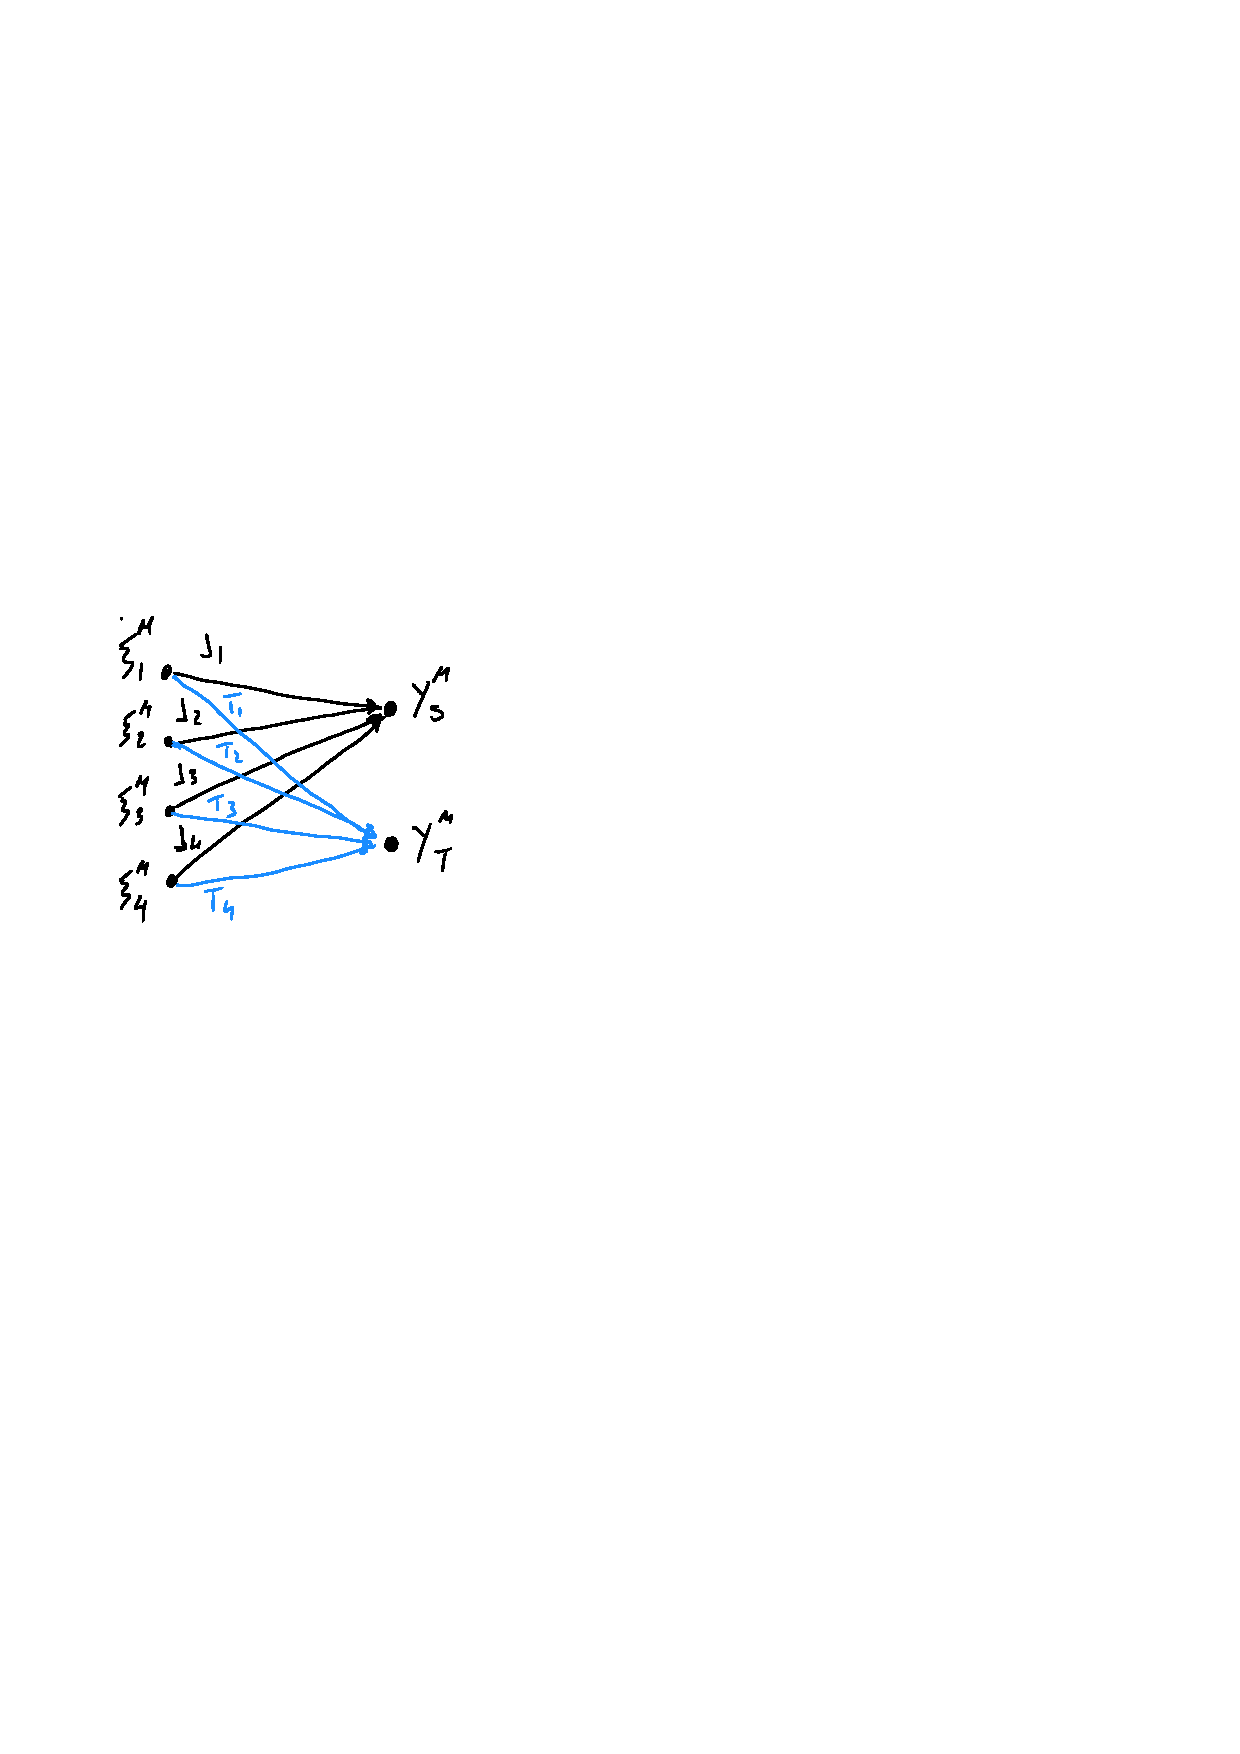
\includegraphics[width = 0.3\textwidth]{./img/perceptron.pdf}
  \begin{center}
    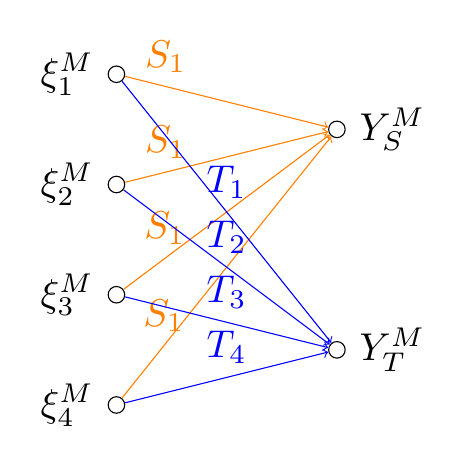
\begin{tikzpicture}[scale=1.4, every node/.style={transform shape}]
    \node[draw, circle, minimum size=0.15cm, inner sep=0.05cm] (A) at (0, 3) {};
    \node[draw, circle, minimum size=0.15cm, inner sep=0.05cm] (B) at (0, 2) {};
    \node[draw, circle, minimum size=0.15cm, inner sep=0.05cm] (C) at (0, 1) {};
    \node[draw, circle, minimum size=0.15cm, inner sep=0.05cm] (D) at (0, 0) {};

    \node[left] at (A.west) {$\xi_1^M$};
    \node[left] at (B.west) {$\xi_2^M$};
    \node[left] at (C.west) {$\xi_3^M$};
    \node[left] at (D.west) {$\xi_4^M$};

    \node[draw, circle, minimum size=0.15cm, inner sep=0.05cm] (Y) at (2, 2.5) {};
    \node[draw, circle, minimum size=0.15cm, inner sep=0.05cm] (Z) at (2, 0.5) {};

    \node[right] at (Y.east) {$Y_S^M$};
    \node[right] at (Z.east) {$Y_T^M$};
  
    % Arrows
    \draw[->, orange] (A) -- (Y) node[pos=0.2, above] {$S_1$};
    \draw[->, orange] (B) -- (Y) node[pos=0.2, above] {$S_1$};
    \draw[->, orange] (C) -- (Y) node[pos=0.2, above] {$S_1$};
    \draw[->, orange] (D) -- (Y) node[pos=0.2, above] {$S_1$};

    \draw[->, blue] (A) -- (Z) node[pos=0.5, above] {$T_1$};
    \draw[->, blue] (B) -- (Z) node[pos=0.5, above] {$T_2$};
    \draw[->, blue] (C) -- (Z) node[pos=0.5, above] {$T_3$};
    \draw[->, blue] (D) -- (Z) node[pos=0.5, above] {$T_4$};

  \end{tikzpicture}
  \end{center}
  \caption{Pictorial representation Student and Teacher Perceptrons.}
\end{figure}



Here, describe the basic setup of the classic \StudentTeacher model, taking an operational view from the perspective of a practitioner training real-world \Student and \Teacher models.  Specifically, we present the \AnnealedApproximation (AA) in a practical light,
and use it explain the difference between computing the \emph{Empirical\GeneralizationError}, $\AVGEMPGE$, for the \emph{\TrueAccuracy}
and for the \emph{\Precision} of a \Teacher model.

\paragraph{Test Error of the Teacher}

We start by describing how to obtain a simple formal expression for the empirical test errors of the \Teacher, first for the \TrueAccuracy.

Let us say we have a model, called \Teacher $(T)$, which maps some \emph{actual} (i.e., correlated) data
$\DATA\in\ADD$ to some known or \emph{true}  labels $(\Ytrue)$
(where,  $\Ytrue$ is, say, an $N$-dimensional vector of binary labels).
We might say that $\Ytrue$ represents the \emph{\GroundTruth} for the problem.
Operationally, we train the \Teacher $T$ to reproduce or at least approximate the true labels $\Ytrue$.
\begin{align}
 T:\DATA\rightarrow \Yt \approx \Ytrue.
\end{align}
If $T$ reproduces the true labels exactly, we might say that the \Teacher has been
trained to \emph{\Interpolation}, and, therefore, $\Yt = \Ytrue$.
Indeed, most models today are trained to \emph{\Interpolation}, and we don't need to
necessarily worry about the difference between the true and the predicted \Teacher labels.
Formally, however, and to understand better the \AA, it is beneficial to discuss the implication
of this distinction.

Following \EQN~\ref{eqn:dnn_energy}, lets say the \Teacher outputs are specified
by an  Energy function $E^{T}_{NN}$
\begin{align}
\label{eqn:T_ENN}
\Yt=E_{NN}(T,\DATA) 
\end{align}
\footnote{Do not confuse the Energy/output function $E_{NN}$ with the energies $\mathbf{\Delta E}$  defined below to represent the ST error function(s).  We refer to outputs of $E_{NN}(\TVEC,\DATA )$, when applied to a data point $\DATA$, as energies because they are effectively un-normalized probabilities for the class outputs (for labels $\Ymu=1$ or $-1$).  }
so that we may write the \emph{Empirical} \AverageTrainingError
$\AVGEMPTE$
as 
\begin{align}
\label{eqn:Eg_train}
\AVGEMPTE:= \frac{1}{N^{train}}\sum_{\mu=1}^{N^{train}}\mathcal{L}[\Ytrain,E_{NN}(T,\DATAtrain)]  .
\end{align}
Ideally, we seek the \emph{True} \AverageGeneralizationError of the \Teacher, denoted  $\AVGGE^{T}$. 
Of course, this is unknowable, but in practice, we estimate $\AVGGE^{T}$ 
by measuring the error of the \Teacher predictions on some test (or hold-out) set $(\DATA^{test}, \MY^{test})$.
We call this the \emph{Empirical \AverageGeneralizationError}, $\AVGEMPGE$, and write
\begin{align}
\label{eqn:Eg_test}
 \AVGGE^{T}\approx \AVGEMPGE:= \frac{1}{\Ntest}\sum_{\mu=1}^{\Ntest}\mathcal{L}[\Ytest,E_{NN}(T,\DATAtest)] .
\end{align}
To measure the error, the loss function $\mathcal{L}$ may be a L1 $(\ell_1)$ or L2 $(\ell_2)$ loss;
whereas for training a model, it is usually something like a cross-entropy loss, but this detail does matter later.

If we don't have a hold-out set, however, we can still estimate $\AVGGE^{T}$ using the \Student-\Teacher approach.

\paragraph{Estimating the Teacher Error with Students: Accuracy vs. Precision}

Imagine training a \Student $(S)$  model (with a similar architecture as $T$, and acting on the same  
dataset $\DATA\in\ADD$), which tries to  reproduce the \Teacher predictions:
\begin{align}
S:\DATA\rightarrow \Ys \approx \Yt  ,
\end{align}
and assume the \Student outputs $\Ys$ are given by the Energy output function $E^{S}_{NN}$
\begin{align}
\label{eqn:S_ENN}
\Ys=E_{NN}(S,\DATA) ,
\end{align}

\begin{figure}[ht] % [h] places the figure approximately here
  \centering
  \resizebox{0.75\textwidth}{!}{

\begin{tikzpicture}

    % Axis
%    \draw[->] (0,0) -- (0,4) node[left] {Predictions};
    \draw[->] (0,0) -- (6,0) node[below] {Value};
    
    % Gaussian distribution
    \draw[thick, red] plot [smooth] coordinates {(1,0) (2,1) (3,3) (4,1) (5,0)};
    
    % Ground Truth line
    \draw[thick, blue] (3,0) -- (3,3.2);
    \node[blue, above] at (2.5,3.2) {\textbf{Accuracy} };
    \draw[->] (2.5,3.) -- (3,3.);
    \node[black, below] at (0.75,3.2) {\textbf{Teacher output} $\Yt$};

    % Accuracy bracket
    \draw[<->, blue, thick] (3,3.2) -- (4,3.2);
    
    % Teacher (high accuracy, low precision)
    \fill[darkgreen] (4,3) circle (0.15);
    \node[right, below] at (5.5,2.9) {\textbf{Ground truth} $\Ytrue$};
    
    % Student outputs (spread)
    \draw[->] (2.5,1) -- (3.5,2);
    \node at (0.75,0.75) {\textbf{Student outputs} $\Ys$};

    % Precision label
    \draw[<->, red, thick] (1,-0.5) -- (5,-0.5);
    \node[red, below] at (3,-0.5) {\textbf{Precision}};
    
    % Bullseye diagram (Right side)
    \begin{scope}[xshift=9cm, yshift=2cm]
        \draw[thick] (0,0) circle (1.8);
        \draw[thick, fill=white] (0,0) circle (1.2);
        \draw[thick, fill=white] (0,0) circle (0.6);

        \fill[blue] (-0.5, 0.0) circle (0.10);
        % Random student outputs
        \foreach \x/\y in {-0.6/0.3, 0.1/-0.7, -0.15/0.5, -0.3/-0.5, -0.75/0.75, -0.9/-0.2} {
            \fill[red] (\x,\y) circle (0.08);
        }
        
        % Teacher dot in center
        \fill[darkgreen] (0,0) circle (0.15);
        
        \node[left] at (2.,-2.5) {\textbf{Bullseye Example}};
    \end{scope}

\end{tikzpicture}
  }
  
\caption{Precision vs. Accuracy}
 \label{fig:precision}
\end{figure}

If the \Teacher is trained to \Interpolation, then the difference between
the \Student and the \Teacher labels 
estimates the true error, i.e., $\Vert\Ys-\Yt\Vert=\Vert\Ys-\Ytrue\Vert$,
and this error is associated with the \TrainingAccuracy of the model in predicting the \GroundTruth.
But if the \Teacher makes some errors, then $\Vert\Ys-\Yt\Vert$
is now estimating the \Precision of the model.
These two situations are depicted in Figure~\ref{fig:precision}.

The \StudentTeacher model also explains why NNs can generalize even even when trained to \Interpolation on noisy data (which has been a source of confusion \cite{Understanding16_TR}).  In this model, the \GeneralizationError  $\AVGGE^{T}$ is a simple function of the overlap $R$ between the \Teacher $T$ and the \Students $S$, i.e., $\AVGGE^{T}\sim \THRMAVG{1-\EPSLR}$.  So even if the \Teacher $T$ is trained on noisy data, as long as there are \Students $S$ with significant overlap $R$ with the \Teacher, the \Teacher \GeneralizationError  $\AVGGE^{T}$  can be considerably small.  For more details, see \cite{MM17_TR_v1}


\paragraph{Learning the Student}
Moving forward, we will always assume the \Teacher is trained to \Interpolation because this
actually corresponds to the \AnnealedApproximation, whereas if the \Teacher makes
errors, we may need to consided  \Quenched averages, explained below.

Imagine now that in order to estimate the empirical \AverageGeneralizationError, $\AVGEMPGE$,
by training a very large number of Students, and computing the average ST error on some test set.
Let us break the data set into training $\DATAtrain$ and test $\DATAtest$ examples, 
train models on the training data (that is, find the optimal model weights), 
and evaluate the $S$ and $T$ models on the test data.

The \Student learning task can be written as in \EQN~(\ref{eqn:dnn_opt})
as the following optimization problem over the training data:
\begin{align}
\underset{\{S'\}}{\argmin}\sum_{\mu=1}^{N^{train}}\mathcal{L}[E_{NN}(S',\DATAtrain),E_{NN}(T,\DATAtrain)]   ,
\label{eqn:ST-learning-task}
\end{align}
%Notice that, at this step, the \Student $S$ and the \Teacher $T$ both depend explicitly on the specific choice of the training data $\DX_{train}$.  
%That is, we could write $S[\DX^{train}], T[\DX^{train}]$.

If the \Teacher is trained to \Interpolation, then the optimization problem in \EQN~\ref{eqn:ST-task} is
training a \Student to reproduce the \GroundTruth labels, so that $\Ys\sim y_{\mu}^{true}$
for both the training and test sets.
\begin{align}
\underset{\{S'\}}{\argmin}\sum_{\mu=1}^{N^{train}}\mathcal{L}[E_{NN}(S',\DATAtrain),\Ytrue]   ,
\label{eqn:ST-learning-intepolation}
\end{align}

But if not, then the \Student is reproducing the possibly
incorrect \Teacher labels, and, importantly, the \Student $S$ now depends explicitly
on how the \Teacher was trained.  That is, we should denote that the learned
\Student explicitly depending on $T$, i.e. $S\rightarrow S[T]$.
This will be important below.

\paragraph{The \AverageGeneralizationError}
In either case, however, we may still estimate the Empirical \AverageGeneralizationError
by replacing the test predictions in \EQN~\ref{eqn:Eg_test} with the student predictions
$y_{\mu}^{test}\rightarrow \Ys$, and then averaging directly over the test data $\DATAtest$
for all possible or available test examples.

If we have a very large number of suitable Students
(say, drawn from some random distribution), then we can try to estimate the 
\AverageGeneralizationError of the \Teacher, i.e., $\TGE^{T}\approx\AVGEMPGE$.
$\AVGEMPGE$ is given by an average loss, the average is 
over all possible Students $N_S$,  and then  over all  $\Ntest$ test data points $\DATAtest\in\mathbf{D}$ 
\begin{align}
  \AVGEMPGE
  &=
  \frac{1}{\Ntest}\sum_{\mu=1}^{\Ntest}
  \frac{1}{N_S}\sum_{S}
  \mathcal{L}[E_{NN}(S,\DATAtest),E_{NN}(T,\DATAtest)]  \\ \nonumber
    &=
  \frac{1}{N_S}\sum_{S}
    \frac{1}{\Ntest}\sum_{\mu=1}^{\Ntest}
    \mathcal{L}[E_{NN}(S,\DATAtest),E_{NN}(T,\DATAtest)] ,
\label{eqn:emp_gen_error}
\end{align}
where (ideally) $\Ntest$ is extremely large.

In Bra-Ket notation, we may also write
\begin{align}
  \AVGEMPGE
  &= \langle \langle \DETOPSTx \rangle_{S} \rangle_{\DXtest}\\ \nonumber
  &= \langle \langle \DETOPSTx \rangle_{\DXtest} \rangle_{S}
\end{align}
where $\DETOPSTx:=\mathcal{L}[E_{NN}(S,\DATAtest),E_{NN}(T,\DATAtest)]$.
For the empirical estimate, it does not matter what order we take the sums in,
but we are not estimating the
the True \AverageGeneralizationError  of the \Teacher, $\AVGGE^{T}$,
unless $T$ is trained to \Interpolation.
For the theoretical estimate, however, the order can be important, and this also depends on
if $T$ is trained to \Interpolation or not.
\footnote{This approach can be likened to the Bootstrap method~\cite{efron1993bootstrap} used for error estimation.  However, the Bootstrap method predominantly emphasizes variations in the input data $\NDX\in\mathbf{D}$, while in this context, we are essentially bootstrapping over the students $S$.}

%\michael{Is this for the optimal values of the parameters in the learning task \EQN~(\ref{eqn:student-learning-task})%?  Presumably not, since we are averaging? }
%\charles{Good question. We do not specify how the hyperparameters are selected.}

\paragraph{Annealed vs. Quenched Averages}
\nred{THIS NEEDS CLEANED UP}
Recall that in the \STATMECH approach to computing errors, we do not break the data into
training and test, but, instead, to obtain the \AverageGeneralizationError, $\AVGGE$, use
the \GeneratingFunction approach. In doing this, we need to compute both the \ThermalAverage
over the model weights ($S,T$), and also take the data average over the entire available model data set $\MDD$
And the order can matter.

In the case where the \Teacher is trained to \Interpolation, may may train the \Student 
independently of \emph{when} the \Teacher.  
But if \Teacher is \emph{not} trained to \Interpolation, then formally we must train the \Teacher
first to obtain target predictions for the \Student.  That is, the \Student formally
depends on the \Teacher, $S[T]$.
The empirical errors in $T$ would then formally depend on the specific instantiation of the data  $\NDXIn\in\MDD$,
and therefore, conceptually imagine that we must first average over the data
before averaging over the weights.
Training to \Interpolation correpsonds conceptually to working with a model
in the \AnnealedApproximation, whereas not correpsonds to \Quenched case.

Practically, when the \Teacher is not trained to \Interpolation, 
we may need to resample the training data and training an ensemble of models to compensate for anomalies in training data (bad labels, noise, etc.) that may cause the underlying model to overfit to the training data.
Theoretically, within \SMOG, this is equivalent to \emph{quenching} the system to the data (a term analogous to quickly cooling a physical system, frezing in any defects).
In contrast, when one \emph{anneals} a physical system, one heats up and cools it down slowly, and repeatedly, thereby removing any defects (of data anomalies for NNs, or material defects in a physical system).

In \STATMECH, one can perform a so-called quenched average using a replica calculation,
effectively removing the dependence on test and/or training data
from the final estimate for $\AVGEMPGE$.
However, the theoretical quenched result may differ significantly from the annealed case when the underlying model is unrealizable~\cite{SST92}. 
This may occur when the training data is very noisy and/or the model architecture is such that it can not correctly predict all the training labels.
In such cases, the model will always have some finite, non-zero Average \TrainingError, $\AVGTE > 0$,
even in the large-$N$ limit of infinite data.  In such a case, this indicates
a highly complex error landscape with many local minima separated by extremely high barriers,
and a slowing down of the dynamics.%
\footnote{In modern ML parlance, one might say the model can not be evaluated at interpolation, although 
in practice such a model might have a zero empirical \TrainingError since it may overfit the specific training data.}
\michael{This seems like important discussion, but it is related to what is going on in Section~\ref{sxn:SMOG_main-spin_glass}; I feel like we should have a minimalistic discussion of things like spin glasses in the main text, and then have a self-contained appendix that goes into it in more detail, since it gets in the way of getting to Section~\ref{sxn:SMOG_main-st_av} and Section~\ref{sxn:matgen}.  }
\charles{This is a minimal discussion.  }

While it is commonplace to train ensembles and/or use cross-validation when training small models (as the above discussion assumes),
this could be extremely expensive and impractical in modern ML, e.g., for very large models like LLMs~\cite{LLMS}.
For such massive NNs, one needs a theory that can detect anomalies in training directly from observations during and/or after training.
This is a hallmark of the \SETOL approach, and it distinguishes \SETOL from the classic \STATMECH approach.
\michael{MM TO DO: Probably move that to the intro.  That is an important par, too imp to be buried here.}
\charles{Not sure.  Intro is already long.  Maybe the conclusions}

%That said, it may be beneficial in practice to use subsamples of the training data to train the \Teacher and the Students
%when, say, the training data has mislabeled and/or noisy data.  With such bad data, the 
%results could be quite different after taking this additional step.
%Indeed, it is exactly these cases where the results differ theoretically as well as in practice.
%We will take a deeper look at such case of noisy data below.

%Importantly, we will not used the quenched form of $\mathcal{E}_{t}^{emp}$ because we will be able todetect
%anomalies in the training data directly by looking at the fitted \SemiEmpirical HT parameter $\alpha$.

be used to estimate the \AverageGeneralizationAccuracy (and not the \Precision),
and which we will refer to more generally as a layer and/or model \Quality.


\paragraph{Generalization Gap vs. Model Quality}
\label{sxn:SMOG_main-model_quality}

We should distinguish between what is typically done in the \SLT literature versus the \STATMECH approaches.
In \SLT, one is typically interested in modeling the \emph{\GeneralizationGap}.
The \GeneralizationGap quantifies the difference between a models performance on training data versus unseen test data:
\begin{align}
  \label{eqn:gen_gap}
  \mathcal{E}^{emp}_{gap}:= \TTE[\DXtrain]- \TGE[\DXtest]
\end{align}
In contrast, in \STATMECH approaches, one considers the \ModelGeneralizationError directly,
which is sometimes called the \ModelQuality in the \SLT literature.
\michael{I think SST looks at generalization error also.  I think this dichotomy isn't quite correct, and it convovles several issues.  It seems most connected with the par around \EQN~\ref{eqn:Qdef} and \EQN~\ref{eqn:GammaQdef}. Maybe we should combine this with that and put is somewhere, removing the incorrect claim/suggestion, and highlighting the ideas in the next par, which are key.
}
\charles{Thats not what this is about.  This is an important section that belongs here.
needs some work}
Model quality is an indication of the models accuracy, precision, recall, or any other relevant metric based on the task at hand.
%Here, we mean that the \ModelGeneralizationError is a measure of the \ModelQuality on such OOD data.

While related, in developing an analytic theory, the \GeneralizationGap and
the \ModelQuality (or \ModelGeneralizationError) require conceptually different approaches.
This is because the  \GeneralizationGap depends on a specific realization of the training data,
whereas our \ModelGeneralizationError will be formulated on a random training data set
(and then corrected later with empirical data).
In this sense, any theory of the \GeneralizationGap  requires a formalism where the
predicted model error is \Quenched to the training data, which is not what we want.
In contrast, the \ModelGeneralizationError  will be formulated using the \AnnealedApproximation (AA),
and is therefore both conceptually and mathematically simpler.
\michael{These ideas seem key; they should either be combined with the par around \EQN~\ref{eqn:Qdef} and \EQN~\ref{eqn:GammaQdef}, or they should be in the intro.}

\nred{Comment on our paper with YQ}




\subsubsection{Theoretical Student-Teacher Average Generalization Error}
\label{sxn:SMOG_main-st_av}

Here, we seek a simple, formal expression for the
\StudentTeacher Average \GeneralizationError, $\AVGSTGE$,
that can be used as the starting point for our extended \SemiEmpirical theory.

%
\begin{figure}[t] %[h] % [h] places the figure approximately here
    \centering
\resizebox{0.75\textwidth}{!}{
\begin{tikzpicture}[
     thick, % Line thickness
    rectnode/.style={rectangle, draw=black, thick, minimum width=6cm, minimum height=2.5cm, rounded corners=0.3cm}, % Rectangular node style with rounded corners
    -> % Arrow style
]

% Nodes with manual positioning
\node[rectnode] (realdata) at (0,0) {%
    \begin{minipage}{6cm}
        \centering
        \textbf{Real Data} \\
        \vspace{0.3cm}
        $\mathbf{x_\mu}, \mathrm{y}_\mu \in \mathbf{D},\;\mu=1, 2, \ldots, n$\\
        $\text{where }$ \\
        $\mathrm{y}_\mu \in \{-1, 1\}$ \\
        $\mathbf{x_\mu}\text{ is real world, correlated data }$ \\
        $\mathbf{x_\mu} \in \mathbb{R}^{M}$, $\Vert\mathbf{x_\mu}\Vert^{2}_{F}=1$
    \end{minipage}
};

\node[rectnode] (modeldata) at (8,0) {%
    \begin{minipage}{6cm}
        \centering
        \textbf{Idealized Data} \\
        \vspace{0.3cm}
        $\boldsymbol{\xi}_\mu, y_\mu \in \mathbf{\mathcal{D}},\;\mu=1, 2, \ldots, \infty$ \\
        $\text{where }$ \\
        $y_\mu \in \{-1, 1\}$ \\
        $\boldsymbol{\xi}_{\mu} \sim \mathcal{N}(0, \tfrac{1}{M} \mathbb{I})$ \\
        $\boldsymbol{\xi}_{\mu}\in \mathbb{R}^{M}$, $\Vert\boldsymbol{\xi}_{\mu}\Vert^{2}_{F}=1$
    \end{minipage}
};

% Arrow between the boxes
\draw[->] (realdata) -- (modeldata);

\end{tikzpicture}
}
\caption{Mapping from a fixed set of $n$
  real-world, correlated data instances $[\mathbf{x},\mathrm{y}]\in\mathbf{D}$
  to an uncorrelated, random model of idealized data   $[\boldsymbol{\xi}, y]\in\mathbf{\mathcal{D}}$, drawn from a Gaussian i.i.d. distribution.
}
    \label{fig:data_mapping}
\end{figure}


\paragraph{The Idealized Data}

To develop a \SemiEmpirical theory of the \Teacher \GeneralizationError, $\TGE^{T}$, 
instead of training and evaluating a NN model using real data $(\DX)$,
we seek a simple, analytical expression with parameters that can be fit to empirical measurements.
So in addition to using a model for our NN, we must specify a idealized model for the data.
In a real NN, the data $\DX$ is correlated, and, in fact, very strongly correlated;
and this is reflected in the layer weight matrices.
However, to be tractable, our starting theoretical expressions use uncorrelated (i.i.d) data.
Formally, we must replace the correlated data 
with some uncorrelated, random model of the data, i.e., $\XVEC\rightarrow\XI$.
As described in Figure~\ref{fig:data_mapping},
our \DataModel is a standard Gaussian $N(0,\sigma^{2}\mathbb{I})$ model for the input data
\begin{align}
\DATA\rightarrow\XImu,\;\;\XImu\in N(0,\sigma^{2}\mathbb{I}) ,
\label{eqn:mwm_replace_1}
\end{align}
where $N(0,\sigma^{2}\mathbb{I})$ denotes a Gaussian distribution with zero mean and variance $\sigma^{2}=\tfrac{1}{M}$,
\and $\XImu$ is normalized such that $\Vert\XImu\Vert^{2}_{F}=1$ for all $\ND$ data vectors.
\michaeladdressed{@charles: I just added a label there, in case you are keeping track of labels.}

We make this distinction between Actual and \ModelData to emphasize that,
later, we will use our so-called \SemiEmpirical procedure to
account for the real correlations in the actual data phenomenologically
by taking some analytical parameter of the theory and fitting it to the real world observations,
here, on the ESD of the NN weight matrices.


\paragraph{The ST Error Model and the Annealed Potential $\EPSLSTx$.}
We now model \Teacher error $\AVGGE^{T}$ with the
\emph{\AverageSTGeneralizationError} $\AVGSTGE$, which is obtained
\michaeladdressed{Is that quite true; doesn't the former involve an extra average, so they are different; see also the comment above on being pedagogically confusing.}
 by \emph{first} computing the ST error function
 %$\Delta\mathbf{E}_{\mathcal{L}}(\SVEC,\TVEC, \XI)$
$\DETOPSTL$
over the set of \emph{all} possible $N$ input examples $\XI$.  Define the data-dependent ST test error function--or Energy difference--as 
\begin{align}
\label{eqn:DE_L}
\DETOPSTL:=\sum_{\mu=1}^{\ND}\mathcal{L}[E_{NN}(\SVEC,\XI_{\mu}),E_{NN}(\TVEC,\XI_{\mu})]  .
\end{align}
where $\mathcal{L}(\SVEC,\TVEC, \XI)$ is simply the $\ell_2$ loss.  This measures the error
between the \Student and the \Teacher; it is zero when their predictions are identical,
$(\Ys=\Yt)$ when $(\XI=\XImu)$, and is nonzero otherwise.

%%5Let us write the Average St \GeneralizationError, $\AVGSTGE$ (formally) as in \EQN~\ref{eqn:finalEgen} as
%%5\begin{align}
%%5\label{eqn:AVGSTGE0}
%%5\AVGSTGE:= & \left\langle\THRMAVG{\Delta\mathbf{E}_{\mathcal{L}}(\SVEC,\TVEC, \XI)}\right\rangle_{\AVGNDXI} 
%%5\end{align}
%%5where we first average over the model data $\NDXI$  and then take a Thermal
%%5average over the \Student weight vectors $\SVEC$.
%%5
%%5We will reduce $\AVGSTGE$ now using the \AnnealedApproximation (AA).
%%5We define two kinds of data-averaged ST errors; the first is used to
%%5define the data-averaged ST \TrainingError, and the second
%%5defines the data-averaged ST test error.
%%5If take the average over the training examples $\XItrain$, we can write
%%5\begin{align}
%%5\label{eqn:ST_train_error}
%%5\langle\Delta\mathbf{E}_{\mathcal{L}}(\SVEC,\TVEC,\XI)\rangle_{\AVGNDXItrain} := \dfrac{1}{\Ntrain}\sum_{\mu=1}^{\Ntrain}\Delta\mathbf{E}_{\mathcal{L}}(\SVEC,\TVEC,\XI_{\mu})
%%5\end{align}
%%5and use this to define the \emph{Model \TrainingError} $\AVGSTTE$.
%%5We dont consider this here,  but it is important for the classic approach;
%%5for a longer discussion, see Section~\ref{sxn:summary_sst92}.
%%5
We aim to derive a simple expression for the  \AverageSTGeneralizationError, $\AVGSTGE$, and to do this, 
we define the  \EffectivePotential for the data-averaged ST \GeneralizationError $\EPSL(\SVEC,\TVEC)$, as in \EQN~\ref{eqn:epsl}, as:
\begin{align}
\label{eqn:STerror}
\EPSLSTx = \langle\DETOPSTL\rangle_{\AVGNDXI}:=\frac{1}{\ND}\int d\mu(\NDXI)\DETOPSTL
\end{align}
The measure $d\mu(\NDXI)$ will end up being a Gaussian measure over $\ND$ samples
(see Appendix~\ref{sxn:summary_sst92}), and the intent is to evaluate it
in the large-$n$ limit, thereby sampling all possible inputs in the model space, $\XI\in\MDD$.

As in Section~\ref{sxn:mathP}, by applying the AA, we can rewrite the \AverageSTGeneralizationError, $\AVGSTGE$:
first, a simple average over all the possible inputs $\XI$; and, 
second, then as a Thermal average over all Students $S$, in the AA, and at high-T 
\begin{align}
\label{eqn:MGE}
\AVGSTGE:=\THRMAVG{\EPSLSTx} .
\end{align}
(Recall that in this regime $\AVGSTGE=\AVGGE^{an,hT}$.)


In the classic \STATMECH approach, the average $\THRMAVG{\cdots}$ is
a \ThermalAverage in the canonical ensemble with $\beta$ fixed,
as explained in Section~\ref{sxn:mathP}.  Here, we will do something similar, as the \Student
average $\THRMAVG{\cdots}$ will be computed from the associated
generating function $\IZG$ for the matrix-generalized case  (i.e., an HCIZ integral defined over all students,
and in both the large-$n$ \Thermodynamic and large-$N$ limits).)

\michael{MM TO DO: The content of this par is good, it just probably needs to be moved.}
Recall that above, the empirical estimate for $\AVGEMPGE$ depended on a
specific instantiation of the model for the training data $\DATAtrain$,
i.e  $\AVGSTGE$ is \Quenched to the training data.
For that reason, for the final result, we needed to take a second,
quenched average over all possible data sets.
Here, we do not need to consider this and always work in the \AnnealedApproximation(AA).
This is because we incorporate
the specific effects of the real-world training data $(\NDX)$ after we derive our formal expressions
by fitting the model parameters to empirical data.
The final expression for $\AVGSTGE$, derived below,
will be generalized to $\AVGNNGE$, matrix-generalization of  the classic \STATMECH formula
for the \LinearPerceptron, in the \Annealed and High-T approximations.
(see Appendix~\ref{sxn:summary_sst92}). 


%%\subsubsection{The Effective Potential as a function of the overlap $(\EPSL(\AVGR))$}
\paragraph{The Annealed Potential as a function of the overlap $(\EPSL(\AVGR))$.}

%%In this subsection, we show that the  data-averaged ST test error function (for the $\mathcal{L}=\ell_2$ loss) is:
%%\begin{align}
%%  \EPSL(\AVGR)=1-R,\;\;\mathcal{L}=\ell_2
%%\end{align}
%%
We want an expression for the data average of the ST test error, from \EQN~\ref{eqn:STerror}, generalized from \Perceptron vectors to NN layer weight matrices.
\michael{MM TO DO: reword that sentence, since it is a bit confusing, since we are vectors here, and I moved the matrix stuff below to the next section.}
For the \Perceptron, one obtains different expressions for the ST error function, depending on 
the type of activation function $h(x)$ in \EQN~\ref{eqn:dnn_energy};
The simplest are the Linear and Boolean \Perceptrons, and
for both (and with $\ell_2$ loss),
 $\EPSL(\SVEC,\TVEC)$ is simply a function of the ST overlap $\AVGR$~\cite{SST92}.
This gives $\EPSLSTx\rightarrow\EPSL(\AVGR)$, where
\begin{align}
  \label{eqn:Rdef}
\AVGR=\SVEC^{\top}\TVEC=\sum_{i=1}^{m}s_{i}t_{i},
\end{align}
which is simply the dot product between the $m$-dimensional \Student $\SVEC$ and \Teacher $\TVEC$ weight vectors, and normalized by the number of training instances $\ND$.
For a \LinearPerceptron~\cite{SST92},% 
\footnote{In the classic approach for the ST model, the theory examined different expressions $\EPSL(\AVGR)$.
For example, one can consider the  Boolean \Perceptron~\cite{SST92,Ros62}, with activation function $h(x)=\mbox{sgn}(x)$, 
i.e., the Heaviside step function. Then, the error is
$
\EPSL(\AVGR)=1 - \dfrac{1}{\pi}\arccos(\AVGR).
$
In both cases, perfect learning occurs when $R=1$~\cite{SST92}.
}
with activation function $h(x)=x$,  the error function is
\begin{align}
\EPSL(\AVGR)=1-\AVGR  .
\label{eqn:LinearPerceptronError}
\end{align}
Since the data vectors are normalized to $1/m$, the average overlap $\AVGR\in[-1,1]$.  And, importantly, the number of free parameters becomes $1$.

\begin{figure}[ht]
\centering

%-------------------------------%
% Left image: 2D Overlap
%-------------------------------%
\begin{minipage}{0.48\linewidth}
\centering
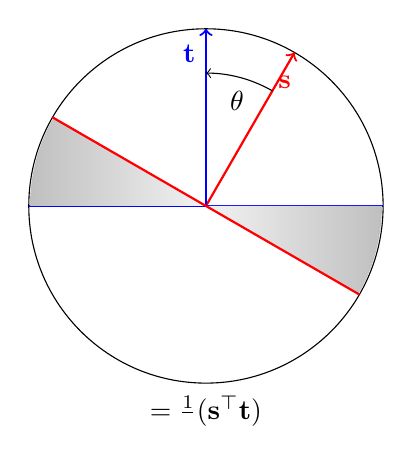
\begin{tikzpicture}[scale=1.5]

    % Circle
    \draw (0, 0) circle (1.5cm);

    % Vectors s (red at 60°) and t (blue at 90°)
    \draw[->,thick,red]  (0,0) -- (60:1.5cm) node[pos=0.7, above right] {\(\mathbf{s}\)};
    \draw[->,thick,blue] (0,0) -- (90:1.5cm) node[pos=0.75, above left] {\(\mathbf{t}\)};

    % Angle theta (between s & t)
    \draw[<-] (0,1.125) arc (90:60:1.125cm) node[pos=0.7, below left] {\(\theta\)};

    % Blue lines (perp. to t = 90°)
    \draw[thick,blue] (0,0) -- (-1.5,0);
    \draw[thick,blue] (0,0) -- ( 1.5,0);

    % Gray shading for overlap region
    \shade[left color=gray!50, right color=gray!10]
      (0,0) -- (-1.49,0) arc (180:150:1.5cm) -- cycle;
    \shade[left color=gray!10, right color=gray!50]
      (0,0) -- (1.49,0) arc (0:-30:1.5cm) -- cycle;

    % Red line(s) perp. to s (60°)
    \draw[thick,red]  (0,0) -- (150:1.5);
    \draw[thick,red]  (0,0) -- (330:1.5); % same as -30°

    % Overlap formula
    \node at (0,-1.75) {\( \AVGR = \frac{1}{\ND} (\mathbf{s}^\top \mathbf{t}) \)};

\end{tikzpicture}
\end{minipage}%
\hfill
%-------------------------------%
% Right image: 3D Overlap (conic sections + wedge)
%-------------------------------%
\begin{minipage}{0.48\linewidth}
\centering
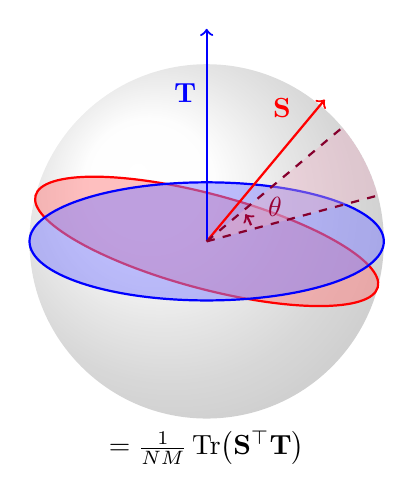
\begin{tikzpicture}[scale=1.5]

    % Light-gray "sphere"
    \shade[ball color=gray!5, opacity=0.3] (0,0) circle (1.5cm);

    % --- Red ellipse for S (unchanged) ---
    \begin{scope}
      \clip (0,0) circle (1.5cm);
      \fill[red!50, opacity=0.5]
        [rotate around={-15:(0,0)}, xscale=1.5, yscale=0.4]
        (0,0) circle (1.0);
    \end{scope}
    \draw[thick, red]
      [rotate around={-15:(0,0)}, xscale=1.5, yscale=0.4]
      (0,0) circle (1.0);

    % --- Blue ellipse for T (CHANGED) ---
    % Make it near-horizontal (rotate=0 or a small angle),
    % and bigger horizontally by increasing xscale significantly.
    \begin{scope}
      \clip (0,0) circle (1.5cm);
      \fill[blue!50, opacity=0.5]
        [rotate around={0:(0,0)},    % CHANGED: no tilt so near x-axis
         xscale=1.5, yscale=0.5]     % CHANGED: bigger horizontally
        (0,0) circle (1.0);
    \end{scope}
    \draw[thick, blue]
      [rotate around={0:(0,0)}, xscale=1.5, yscale=0.5]
      (0,0) circle (1.0);

    % Vectors S (red) & T (blue, vertical & longer)
    \draw[->,thick,red]  (0,0) -- (1.0,1.2)
      node[pos=0.8, above left]  {\(\mathbf{S}\)};
    \draw[->,thick,blue] (0,0) -- (0,1.8)
      node[pos=0.7, left] {\(\mathbf{T}\)};

    % Remove old "theta" arcs

    % -- Fill a wedge (solid angle) in purple --
    \begin{scope}
      \clip (0,0) circle (1.5cm);
      % Let’s pick a narrower wedge from ~15° to ~40°
      \fill[purple!30, opacity=0.4]
        (0,0)
         -- (15:1.5cm)
         arc [start angle=15, end angle=40, radius=1.5cm]
         -- cycle;
    \end{scope}

    % Dashed wedge boundaries
    \draw[thick, dashed, purple!70!black] (0,0) -- (15:1.5cm);
    \draw[thick, dashed, purple!70!black] (0,0) -- (40:1.5cm);

    % Single arc to label theta
    \draw[->, thick, purple!80!black]
      (20:0.4) arc[start angle=20, end angle=35, radius=0.4];
    \node[purple!80!black] at (27:0.65) {\(\theta\)};

    % Overlap formula
    \node at (0,-1.75) {\( \AVGR = \frac{1}{NM} \,\mathrm{Tr}\bigl(\mathbf{S}^\top \mathbf{T}\bigr) \)};

\end{tikzpicture}
\end{minipage}

% Main caption
\caption{Comparison of 2D and 3D representations of the vector and matrix Student--Teacher overlap \(R\).
\textbf{Left:} \(\AVGR = \tfrac{1}{\ND}\mathbf{s}^\top \mathbf{t}\).  Averaged over $\ND$ data samples (implicitly normalized to $1/m$).
\textbf{Right:} \(R = \tfrac{1}{NM}\,\mathrm{Tr}\bigl(\mathbf{S}^\top\mathbf{T}\bigr)\) with conic sections on the sphere (red \(\mathbf{S}\), blue \(\mathbf{T}\)), plus a purple wedge for the angle.  Averaged over matrix dimensions $N$ and $M$ (implicitly normalized over the data $1/\ND$).}
\label{fig:overlaps}
\end{figure}

%\caption{Comparison of 2D and 3D representations of matrix overlap $R$. (a) 2D visualization of vector overlap $R = \cos(\theta) $.
%  (b) 3D visualization of matrix overlap $R = \Trace{\frac{1}{N^2} \SMAT^\top \TMAT $ with solid angle $R$.}



%%\subsubsection{Derivation of the  ST error $(\EPSL(\AVGR))$ for the Linear Perceptron}
\paragraph{Derivation of the  ST error $(\EPSL(\AVGR))$ for the Linear Perceptron.}
%\nred{WARNING: there may be some mistakes here}
To derive \EQN~\ref{eqn:LinearPerceptronError},
define the data-dependent ST error (\EQN~\ref{eqn:DE_L}) in terms of an $\ell_2$ loss function
%\begin{align}
%\nonumber
%\Delta \mathbf{E}_{\ell_2}(\SVEC,\TVEC,\XI) = & \frac{1}{2} (\Ys - \Yt)^T(\Ys - \Yt) 
%   = 1 - (\YsVEC)^{\top}(\YtVEC) \\ 
%\label{eqn:deriveSTerror}
%   =&  1 - \eta(\XI),
%\end{align}
\red{THIS SECTION HAS SOME TYPOS}

\begin{align}
\nonumber
\DETOPSTLL= & \frac{1}{2} (\YsVEC - \YtVEC)^{\top} (\YsVEC - \YtVEC) \\
\nonumber
=& \frac{1}{2} \big[(\YsVEC)^{\top} \YsVEC - 2 (\YsVEC)^{\top} \YtVEC + (\YtVEC)^{\top} \YtVEC \big] \\
\nonumber
=& \ND - (\YsVEC)^{\top} (\YtVEC) \\
\label{eqn:deriveSTerror}
=& \ND- \ETA(\SVEC,\TVEC,\red{\NDXI}),
\end{align}
where we define $\ETA(\SVEC,\TVEC,\red{\NDXI}):=\mathbf{y}_{S}^{\top}\mathbf{y}_{T}$, called
the \emph{data-dependent \SelfOverlap}; we expand this below.
The expression $\ETA(\SVEC,\TVEC,\XI)$ is analogous to the ST overlap $R$, but before the data has been integrated out.
It is convenient to work directly with
the \SelfOverlap $\ETA(\SVEC,\TVEC,\XI)$ because it will appear later in \EQN~\ref{eqn:eta_mat_avg_def} (in Section~\ref{sxn:matgen}), 
when formulating the matrix-generalized overlap operator~$\OVERLAP$.

In defining $\ETA(\SVEC,\TVEC,\XI)$, we replace the labels $(\mathbf{y}_{S},\mathbf{y}_{T})$ with the Energy functions $E_{NN}$  that generate them, giving an expression in terms of the weights $(\SVEC,\TVEC)$ and the Gaussian data variables $(\XI)$. We will then integrate out the data variables, leaving an expression just in terms of the weights.  
Using the $E_{NN}$ Energy generating or output function (\EQN~\ref{eqn:dnn_energy}, \ref{eqn:S_ENN}, \ref{eqn:T_ENN}), we can replace the label vectors $\YtVEC,\YsVEC$ as
\begin{align}
\YsVEC=\SVEC^{\top}\XI,\;\;
\YtVEC=\TVEC^{\top}\XI  ,
\end{align}
which gives
\begin{align}
  \label{eqn:eta_vec_xi_def}
\ETA(\SVEC,\TVEC,\XI) =\red{\sum_{\mu=1}^{\ND}} (\SVEC^{\top}\XI)^{\top} (\TVEC^{\top}\XI) = \red{\sum_{\mu=1}^{\ND}}\XI^{\top}_{\red{\mu}}  (\SVEC^{\top} \TVEC )\XI_{\red{\mu}} 
\end{align}
\red{THIS SECTION HAS SOME TYPOS}
or, more simply, after integrating over the data, we have the \emph{data-independent \SelfOverlap}
\begin{align}
  \label{eqn:eta_vec_avg_def}
\ETA(\SVEC,\TVEC) = \langle\ETA(\SVEC,\TVEC,\XI)\rangle_{\AVGNDXI}=\SVEC^{\top} \TVEC 
\end{align}

We want to evaluate this as an \EffectivePotential $\EPSL(\AVGR)$ for the data-averaged ST test error, as in \EQN~\ref{eqn:STerror}.
To do this, we need to compute the average or \ExpectedValue over all $\ND$ possible input data vectors $\NDXI (i.e., $d\mu(\NDXI)=\mathcal{D}\NDXI P(\NDXI)$).
%
\red{BELOW IS WRONG NEEDS FIED}
\begin{align}
 \langle\DETOPSTLL\rangle_{\AVGNDXI}  
   = & \int d\mu(\NDXI)(1-\ETA(\XI)) \\ \nonumber
   = & \int d\mu(\NDXI)(1-\XI^{\top}\tfrac{1}{\ND}\SVEC^{\top}\TVEC\XI) \\ \label{eqn:XI_ST} 
   = & \int d\mu(\NDXI)-\int d\mu(\NDXI)\XI^{\top}\tfrac{1}{\ND}\SVEC^{\top}\TVEC\XI)  \\ \nonumber
   = & 1 - \int d\mu(\NDXI)\XI^{\top}\tfrac{1}{\ND}\SVEC^{\top}\TVEC\XI \\ \nonumber
   = & 1 - \int d\mu(\XI)\XI^{\top} \AVGR\XI \\ \nonumber
   = &1 - \AVGR\int d\mu(\XI)\XI^{\top}\XI,
\end{align}
where this holds because the elements of $\XI$ are i.i.d.
Since $d\mu(\NDXI)$ is a measure over a (multi-variate) Gaussian distribution,
The data vectors $\XI$ are normalized (See Section~\ref{app:st-gen-err-annealed-ham}) such that the second term on the R.H.S. is unity and we recover (i.e.,\EQN~\ref{eqn:epsl})
\begin{align}
\label{eqn:e0}
\EPSL(\AVGR)=\langle\DETOPSTLL\rangle_{\AVGNDXI} =  1 - \AVGR .
\end{align}


In traditional \STATMECH (e.g., \cite{SST92}), one is interested in how the \emph{\TotalModelGeneralizationError} $\TGE(\AVGR)$ depends on $\AVGR$.
With these simple error functions, \EQN~\ref{eqn:MGE} reduces to a function over $\AVGR$,
and the \AverageSTGeneralizationError $\STGE(\AVGR)$ is then obtained by averaging over the Students 
\begin{align}
\label{eqn:AVGSTGE_R}
\AVGSTGE(\AVGR)=\THRMAVG{\EPSL(\AVGR)}=
\THRMAVG{1-\langle\ETA(\SVEC,\TVEC,\XI)\rangle_{\AVGNDXI}}=
\THRMAVG{1-\ETA(\SVEC,\TVEC)}=
\THRMAVG{1-\SVEC^{\top}\TVEC}=
\THRMAVG{(1-\AVGR)}  ,
\end{align}
where $\THRMAVG{\cdots}$ is a \ThermalAverage over the \Student weight vector $\SVEC$.

The \ModelQuality for the ST \Perceptron, $\Q^{ST}$
is just the \AverageGeneralizationAccuracy, so we can write
\begin{align}
\label{eqn:QST_final}
\Q^{ST} := 1 - \AVGSTGE(\AVGR) 
       = \THRMAVG{1 - \EPSL(\AVGR)} 
       = \THRMAVG{\langle\ETA(\SVEC, \TVEC, \XI)\rangle_{\AVGNDXI}} 
       = \THRMAVG{\ETA(\SVEC, \TVEC)} 
       = \THRMAVG{\SVEC^{\top}\TVEC} 
       = \THRMAVG{\AVGR}.
\end{align}
\EQN~\ref{eqn:QST_final} is the starting point for deriving a \SEMIEMP theory for the \WW quality metrics (\ALPHA,\ALPHAHAT);
see Section~\ref{sxn:matgen_mlp3}.
To generalize this expression, we will start with the \SelfOverlap $\ETA(\SMAT,\TMAT,\XI)$ for a
\MultiLayerPerceptron (MLP3) in Section~\ref{sxn:matgen}.

Before doing this, however, we note that 
we can obtain this expression for $\STGE$ by defining the
\AnnealedHamiltonian $\HANHT(\AVGR)$, at high-Temperature, as in Section~\ref{sxn:mathP}, \EQN~\ref{eqn:Gan_highT_final}.
\nred{I H a fcn or avg R?}
Indeed, it is really $\HANHT(\AVGR)=\EPSL(\AVGR)$ that we must generalize to the matrix case, which we do (using a technique
similar to a Replica calculation, but still in the AA).
For more details, see Appendix~\ref{sxn:summary_sst92}.
(In particular, doing this allows us to define the normalization needed later for the \TRACELOG condition).
\michaeladdressed{MM TO DO: still to work on this par.}


\begin{table}[t]
  \raggedright
\hspace*{-1.5cm}% Adjust this value as needed
\renewcommand{\arraystretch}{1.25} % Increase line spacing in table
\begin{tabular}{|c|c|c|c|}
  \hline
  Quantity & Traditional \SMOG & \makecell{\LinearPerceptron \\ in Traditional \SMOG} & \makecell{Matrix Generalization \\ for \SETOL} \\ \hline

  Total (Idealized) Data Error 
    & $\DETOPXI$ (\ref{eqn:detox})
    & $\DETOPSTL$ (\ref{eqn:deriveSTerror}) 
    & $\DETOPNN$ (\ref{eqn:DE2}) \\ \hline

   Annealed Hamiltonian
    & $\HANHT=\EPSLw$ (\ref{eqn:epsl}) 
    & $\GANHTR=\EPSLSTx=1-\AVGR$ (\ref{eqn:epslR}) 
  & $\GANMATHT = N(\IM-\OVERLAP)$ (\ref{eqn:GANHTmatR}) \\

  (Data-Averaged Error) 
    & (AA, at high-T) 
    & (and at \LargeN) 
    & (only for a layer)  \\ \hline

    \SelfOverlap 
    & $\ETAw = 1-\EPSLw$~(\ref{eqn:def_eta})

    & $\ETA(\SVEC,\TVEC)=\SVEC^{\top}\TVEC$ (\ref{eqn:eta_vec_avg_def})
    & $\ETA(\SMAT,\TMAT)=\tfrac{1}{N}\SMAT^{\top}\TMAT$ (\ref{eqn:eta_mat_avg_def})  \\ \hline
    \hline

  \ModelQuality 
    & $\Q:=1-\AVGGE$ 
    & $\Q^{ST}:=1-\AVGGE^{ST}$ (\ref{eqn:model_qualities})
   & $\Q^{NN}:=1-\AVGGE^{NN}$  (\ref{eqn:model_qualities})\\ 

  in terms of \LayerQuality
    & 
    & 
   & $\Q^{NN}:=\prod_{L} \Q^{NN}_{L}$ \\ \hline
\end{tabular}
\caption{Summary of key quantities compared across traditional \SMOG models,  the \Student-\Teacher (ST) \LinearPerceptron--in the \AnnealedApproximation
(AA) and at high-Temperature (high-T) and at \LargeN in $\ND$, and the matrix-generalized forms as the starting point to frame \SETOL.
The total ST Error of Energy, $\DELBF$, represents the difference (squared) between the model and its labels for the ST model between
the \Student and \Teacher predictions.
The \AnnealedHamiltonian is the Energy function for this Error after it is averaged over the model for the training data
(an $\ND$-dimensional i.i.d. idealized Gaussian dataset,  $\NDXIn$).
In the AA, the \AnnealedHamiltonian is equal to the \EffectivePotential.  For the ST model,  this is one minus the average overlap, $\HANHT(R)=(1-\AVGR)$;
for the \SETOL, this is  the ($M$-dimensional) identity minus the overlap operator/matrix, $\HANHT(\OVERLAP)=N(\IM-\OVERLAP)$. 
The \SelfOverlap $\eta(\cdots)$ is used to describe the Accuracy (as opposed to the Error) for both the ST model and
its matrix-generalized form.
%Notice that $\eta(\XI)$, as defined,  has not yet been averaged over the model data $\XI^{N}$.
Finally, the different forms of the \Quality are defined.  Generally speaking, the \Quality $\Q$ is an approximation to some measure
of $1$ minus the \AverageGeneralizationError, $\Q:=1-\AVGGE$ (in the AA, at high-T, at \LargeN, and with whatever else
approximations are applied).
For the ST model, having just 1 layer, the \ModelQuality and the \LayerQuality are the same, and denoted $\Q^{ST}$.
For \SETOL, the \ModelQuality $\Q^{NN}$ is a product of individual \LayerQualities $\Q^{NN}_{L}$.
(Note that the  final \SETOL \LayerQuality $\Q$ is defined in terms of the \LayerQualitySquared $\QT$,
and the starting point for this is expressed with the \LayerQualitySquared Hamiltonian $\HBARE=\OLAPTOLAP$.
}
\label{table:quantities_general_vect_matrix}
\end{table}


\clearpage

%
\subsection{Generalization Gap vs. Model Quality}
\label{sxn:SMOG_main-model_quality}

In this subsection, we should distinguish between what is typically done in the \SLT literature versus the \STATMECH approaches.
In \SLT, one is typically interested in modeling the \emph{\GeneralizationGap}.
The \GeneralizationGap quantifies the difference between a models performance on training data versus unseen test data:
\begin{align}
  \label{eqn:gen_gap}
  \mathcal{E}^{emp}_{gap}:= \TTE[\DXtrain]- \TGE[\DXtest]
\end{align}
In contrast, in \STATMECH approaches, one considers the \ModelGeneralizationError directly,
which is sometimes called the \ModelQuality in the \SLT literature.
\michael{I think SST looks at generalization error also.  I think this dichotomy isn't quite correct, and it convovles several issues.  It seems most connected with the par around \EQN~\ref{eqn:Qdef} and \EQN~\ref{eqn:GammaQdef}. Maybe we should combine this with that and put is somewhere, removing the incorrect claim/suggestion, and highlighting the ideas in the next par, which are key.
}
\charles{Thats not what this is about.  This is an important section that belongs here.
needs some work}
Model quality is an indication of the models accuracy, precision, recall, or any other relevant metric based on the task at hand.
%Here, we mean that the \ModelGeneralizationError is a measure of the \ModelQuality on such OOD data.

While related, in developing an analytic theory, the \GeneralizationGap and
the \ModelQuality (or \ModelGeneralizationError) require conceptually different approaches.
This is because the  \GeneralizationGap depends on a specific realization of the training data,
whereas our \ModelGeneralizationError will be formulated on a random training data set
(and then corrected later with empirical data).
In this sense, any theory of the \GeneralizationGap  requires a formalism where the
predicted model error is \Quenched to the training data, which is not what we want.
In contrast, the \ModelGeneralizationError  will be formulated using the \AnnealedApproximation (AA),
and is therefore both conceptually and mathematically simpler.
\michael{These ideas seem key; they should either be combined with the par around \EQN~\ref{eqn:Qdef} and \EQN~\ref{eqn:GammaQdef}, or they should be in the intro.}

\nred{Comment on our paper with YQ}


%
\subsection{Bad Training Data and the Spin Glass Phase}
\label{sxn:SMOG_main-spin_glass}

\charles{FIRST PASS ON THIS SECTION}

\michael{Some of this material is redundant with the above.  I think we should have some modularized discussion of these issues, but pputting it here here seems to distract/dealy the reader.}

When training data is of low quality—whether due to mislabeling, inherent noise, or a generally unrealizable task—neural networks exhibit behavior fundamentally different from predictions by \StatisticalLearningTheory (\SLT). In \SLT, the focus is often on the \GeneralizationError as a function of model complexity and data distribution. However, classic \STATMECH analysis shows that when data is mislabeled or the problem is fundamentally unsolvable, the behavior of the neural network changes, revealing a notable divergence between unquenched (annealed) and quenched analyses.

In such cases, the neural network perceptron layer may enter what is known as the spin glass phase. This phase signifies a highly disordered state in which the network struggles to find stable, consistent solutions, akin to the frustrated interactions seen in spin glass systems in physics.
Analogously, the \SETOL approach theory posits that, under these challenging conditions, the NN layer operates in a distinct regime,
particularly when the \HTSR parameter  $\alpha < 2$ and the \TRACELOG condition $\mbox{detX} < 0$.
These two independent, complementary conditions both places the layer within the \emph{\VeryHeavyTailed} (VHT) Universality class,
seems empirically to reflect instability and overfitting, and presumably on specific data instances or features.

This phenomenon diverges sharply from traditional learning theories, underscoring the role of data quality in neural network
behavior and offering a unique perspective for understanding overfitting and generalization in deep learning systems.



%\nred{REWORKED THIS SECTION; stil in progress}
\charles{If we include this section, we should cite the specific results from the old SST paper, including a plot
and we should cite our older paper.   but, importantly, we should prep the read for the empirical results in
section 6 on correlation traps and glassy dynamics, and we should discuss $F$ become non-extensive and/or non-analytic}
\subsection{Bad Training Data and the Spin Glass Phase}
\label{sxn:SMOG_main-spin_glass}

When training data is of low quality---whether due to mislabeling, inherent noise, or a generally unrealizable task---neural networks exhibit behavior that diverges sharply from what \SLT\ would predict under cleaner data assumptions. In \SLT, one typically studies the \GeneralizationError as a function of model complexity and data distribution, often assuming that data is realizable. By contrast, a \STATMECH-based analysis highlights that, when data itself is contradictory or highly random, the network can enter a \emph{spin glass--like phase}, marked by frustration and disorder.

\paragraph{From Annealed to Quenched: The Role of Disorder.}
In the \StudentTeacher\ model, the \AnnealedApproximation (AA) supposes that one can simply average over data disorder. However, with \emph{bad} training data---random or conflicting labels---that assumption breaks down. A \emph{quenched} treatment, which holds the disorder fixed while averaging over model parameters, shows that the perceptron's loss landscape fragments into many local minima, much like a spin glass in physics, and characterized bv \emph{Frustration}.

Frustration can arise when facing mislabeled or contradictory training examples, leading to:
\begin{itemize}
\item Multiple ``almost-satisfactory'' weight matrics coexist, each misclassifying a different subset of examples.
\item The abundance of local minima is characteristic of a \emph{spin glass} phase: no single global minimum stands out; the model can get ``stuck'' in a metastable configuration.
\end{itemize}

In such disordered regimes, the AA often underestimates the difficulty of learning.
In contrast, a fully \emph{quenched} theoretical analysis captures
how small random variations in data can drastically alter the learned weights $\WVEC$':
\begin{itemize}
\item \emph{Annealed}: Increasing the number of training examples always decreases training error, i.e. $(N \gg 1) \rightarrow (\DETOT\approx 0)$, and, also the generalization or test error.  \nred{comment on DD?}
\item \emph{Quenched}: In a spin glass regime, contradictory data can trap the model; adding more data may not improve (or can even worsen) generalization.
\end{itemize}

\paragraph{Practical Considerations}

Such \emph{spin glass} behavior highlights the pivotal role of data quality. Even if the network has vast capacity, it cannot reliably generalize when the dataset is fundamentally inconsistent. Instead, the model remains in a ``frozen'' disordered state:
\begin{itemize}
\item \emph{Overfitting}: The perceptron might merely memorize certain random labels, rather than extracting meaningful structure.
\item \emph{Instability}: Small perturbations in the data can dramatically change the final weights, reflecting a glassy landscape of solutions.
\item \emph{Phase Transitions}: As the fraction of contradictory (or noise-corrupted) data increases, one observes a shift from a ``learnable'' phase to a frustrated, spin-glass--like phase.
\end{itemize}

Hence, this spin glass analogy clarifies why purely annealed approaches can fail for mislabeled or unrealizable tasks: sufficiently disordered data can lock the model into a \emph{glassy} configuration, where it nominally ``fits'' parts of the data but loses coherent generalization capability. Detecting these heavy-tailed indicators ($\alpha < 2$) connects insights from \STATMECH\ to modern deep learning challenges.

%\subsection{Theoretical Student-Teacher Average Generalization Error $(\AVGSTGE)$, }
\label{sxn:SMOG_main-st_av}

In this subsection, we seek a simple, formal expression for the
\StudentTeacher Average \GeneralizationError, $\AVGSTGE$,
that can be used as the starting point for our extended \SemiEmpirical theory.

%
\begin{figure}[t] %[h] % [h] places the figure approximately here
    \centering
\resizebox{0.75\textwidth}{!}{
\begin{tikzpicture}[
     thick, % Line thickness
    rectnode/.style={rectangle, draw=black, thick, minimum width=6cm, minimum height=2.5cm, rounded corners=0.3cm}, % Rectangular node style with rounded corners
    -> % Arrow style
]

% Nodes with manual positioning
\node[rectnode] (realdata) at (0,0) {%
    \begin{minipage}{6cm}
        \centering
        \textbf{Real Data} \\
        \vspace{0.3cm}
        $\mathbf{x_\mu}, \mathrm{y}_\mu \in \mathbf{D},\;\mu=1, 2, \ldots, n$\\
        $\text{where }$ \\
        $\mathrm{y}_\mu \in \{-1, 1\}$ \\
        $\mathbf{x_\mu}\text{ is real world, correlated data }$ \\
        $\mathbf{x_\mu} \in \mathbb{R}^{M}$, $\Vert\mathbf{x_\mu}\Vert^{2}_{F}=1$
    \end{minipage}
};

\node[rectnode] (modeldata) at (8,0) {%
    \begin{minipage}{6cm}
        \centering
        \textbf{Idealized Data} \\
        \vspace{0.3cm}
        $\boldsymbol{\xi}_\mu, y_\mu \in \mathbf{\mathcal{D}},\;\mu=1, 2, \ldots, \infty$ \\
        $\text{where }$ \\
        $y_\mu \in \{-1, 1\}$ \\
        $\boldsymbol{\xi}_{\mu} \sim \mathcal{N}(0, \tfrac{1}{M} \mathbb{I})$ \\
        $\boldsymbol{\xi}_{\mu}\in \mathbb{R}^{M}$, $\Vert\boldsymbol{\xi}_{\mu}\Vert^{2}_{F}=1$
    \end{minipage}
};

% Arrow between the boxes
\draw[->] (realdata) -- (modeldata);

\end{tikzpicture}
}
\caption{Mapping from a fixed set of $n$
  real-world, correlated data instances $[\mathbf{x},\mathrm{y}]\in\mathbf{D}$
  to an uncorrelated, random model of idealized data   $[\boldsymbol{\xi}, y]\in\mathbf{\mathcal{D}}$, drawn from a Gaussian i.i.d. distribution.
}
    \label{fig:data_mapping}
\end{figure}


\paragraph{The Data Model.}

To develop a \SemiEmpirical theory of the \Teacher \GeneralizationError, $\TGE^{T}$, 
instead of training and evaluating a NN model using real data $(\DX)$,
we seek a simple, analytical expression with parameters that can be fit to empirical measurements.
So in addition to using a model for our NN, we must specify a model for the data.
In a real NN, the data $\DX$ is correlated, and, in fact, very strongly correlated;
and this is reflected in the layer weight matrices.
However, to be tractable, our starting theoretical expressions use uncorrelated (i.i.d) data.
Formally, we must replace the correlated data 
with some uncorrelated, random model of the data, i.e., $\XVEC\rightarrow\XI$.
As described in Figure~\ref{fig:data_mapping},
our \DataModel is a standard Gaussian $N(0,1)$ model for the input data
\begin{align}
\DATA\rightarrow\XImu,\;\;\XImu\in N(0,1) ,
\label{eqn:mwm_replace_1}
\end{align}
where $N(0,1)$ denotes a Gaussian distribution with zero mean and unit variance,
\and $\XImu$ is normalized such that $\Vert\XImu\Vert=\tfrac{1}{M}$ for all $N$ data vectors.
\michaeladdressed{@charles: I just added a label there, in case you are keeping track of labels.}

We make this distinction between Actual and \ModelData to emphasize that,
later, we will use our so-called \SemiEmpirical procedure to
account for the real correlations in the actual data phenomenologically
by taking some analytical parameter of the theory and fitting it to the real world observations,
here, on the ESD of the NN weight matrices.


\paragraph{The ST Error Model and the Annealed Potential $\EPSLSTx$.}
We now model \Teacher error $\AVGGE^{T}$ with the
\emph{\AverageSTGeneralizationError} $\AVGSTGE$, which is obtained
\michaeladdressed{Is that quite true; doesn't the former involve an extra average, so they are different; see also the comment above on being pedagogically confusing.}
 by \emph{first} computing the ST error function
 %$\Delta\mathbf{E}_{\mathcal{L}}(\SVEC,\TVEC, \XI)$
$\DETOPSTL$
over the set of \emph{all} possible $N$ input examples $\XI$.  Define the data-dependent ST test error function
--or Energy difference--as 
\begin{align}
\label{eqn:DE_L}
%\Delta\mathbf{E}_{\mathcal{L}}(\SVEC,\TVEC, \XI):=\sum_{\mu=1}^{N}\mathcal{L}[E_{NN}(\SVEC,\XI_{\mu}),E_{NN}(\TVEC,\XI_{\mu})]  .
\DETOPSTL:=\sum_{\mu=1}^{N}\mathcal{L}[E_{NN}(\SVEC,\XI_{\mu}),E_{NN}(\TVEC,\XI_{\mu})]  .
\end{align}
where $\mathcal{L}(\SVEC,\TVEC, \XI)$ is simply the $\ell_2$ loss.  This measures the error
between the \Student and the \Teacher; it is zero when their predictions are identical,
$(\Ys=\Yt)$ when $(\XI=\XImu)$, and is nonzero otherwise.

%%5Let us write the Average St \GeneralizationError, $\AVGSTGE$ (formally) as in \EQN~\ref{eqn:finalEgen} as
%%5\begin{align}
%%5\label{eqn:AVGSTGE0}
%%5\AVGSTGE:= & \left\langle\THRMAVG{\Delta\mathbf{E}_{\mathcal{L}}(\SVEC,\TVEC, \XI)}\right\rangle_{\AVGNDXI} 
%%5\end{align}
%%5where we first average over the model data $\NDXI$  and then take a Thermal
%%5average over the \Student weight vectors $\SVEC$.
%%5
%%5We will reduce $\AVGSTGE$ now using the \AnnealedApproximation (AA).
%%5We define two kinds of data-averaged ST errors; the first is used to
%%5define the data-averaged ST \TrainingError, and the second
%%5defines the data-averaged ST test error.
%%5If take the average over the training examples $\XItrain$, we can write
%%5\begin{align}
%%5\label{eqn:ST_train_error}
%%5\langle\Delta\mathbf{E}_{\mathcal{L}}(\SVEC,\TVEC,\XI)\rangle_{\AVGNDXItrain} := \dfrac{1}{\Ntrain}\sum_{\mu=1}^{\Ntrain}\Delta\mathbf{E}_{\mathcal{L}}(\SVEC,\TVEC,\XI_{\mu})
%%5\end{align}
%%5and use this to define the \emph{Model \TrainingError} $\AVGSTTE$.
%%5We dont consider this here,  but it is important for the classic approach;
%%5for a longer discussion, see Section~\ref{sxn:summary_sst92}.
%%5
We aim to derive a simple expression for the  \AverageSTGeneralizationError, $\AVGSTGE$, and to do this, 
we define the  \EffectivePotential for the data-averaged ST \GeneralizationError $\EPSL(\SVEC,\TVEC)$, as in \EQN~\ref{eqn:epsl}, as:
\begin{align}
\label{eqn:STerror}
%\EPSLSTx = \langle\Delta\mathbf{E}_{\mathcal{L}}(\SVEC,\TVEC,\XI)\rangle_{\AVGNDXI}:=\frac{1}{N}\int d\mu(\NDXI)\Delta\mathbf{E}_{\mathcal{L}}(\SVEC,\TVEC,\XI)  ,
\EPSLSTx = \langle\DETOPSTL\rangle_{\AVGNDXI}:=\frac{1}{N}\int d\mu(\NDXI)\DETOPSTL
\end{align}
The measure $d\mu(\NDXI)$ will end up being a Gaussian measure over $N$ samples
(see Appendix~\ref{sxn:summary_sst92}), and the intent is to evaluate it
in the large-$N$ limit, thereby sampling all possible inputs in the model space, $\XI\in\MDD$.

As in \EQN~\ref{eqn:finalEgen} (Section~\ref{sxn:mathP}), by applying the AA, we can rewrite the \AverageSTGeneralizationError, $\AVGSTGE$:
first, a simple average over all the possible inputs $\XI$; and, 
second, then as a Thermal average over all Students $S$, in the AA, and at high-T 
\begin{align}
\label{eqn:MGE}
\AVGSTGE:=\THRMAVG{\EPSLSTx} .
\end{align}
(Recall that in this regime $\AVGSTGE=\AVGGE^{an,hT}$.)


In the classic \STATMECH approach, the average $\THRMAVG{\cdots}$ is
a \ThermalAverage in the canonical ensemble with $\beta$ fixed,
as explained in Section~\ref{sxn:mathP}.  Here, we will do something similar, as the \Student
average $\THRMAVG{\cdots}$ will be computed from the associated
generating function $\IZG$ for the matrix-generalized case  (i.e., an HCIZ integral defined over all students,
and in the large-$N$ limit).)

\michael{MM TO DO: The content of this par is good, it just probably needs to be moved.}
Recall that above, the empirical estimate for $\AVGEMPGE$ depended on a
specific instantiation of the model for the training data $\DATAtrain$,
i.e  $\AVGSTGE$ is \Quenched to the training data.
For that reason, for the final result, we needed to take a second,
quenched average over all possible data sets.
Here, we do not need to consider this and always work in the \AnnealedApproximation(AA).
This is because we incorporate
the specific effects of the real-world training data $(\NDX)$ after we derive our formal expressions
by fitting the model parameters to empirical data.
The final expression for $\AVGSTGE$, derived below,
will be generalized to $\AVGNNGE$, matrix-generalization of  the classic \STATMECH formula
for the \LinearPerceptron, in the \Annealed and High-T approximations.
(see Appendix~\ref{sxn:summary_sst92}). 


%%\subsubsection{The Effective Potential as a function of the overlap $(\EPSL(R))$}
\paragraph{The Annealed Potential as a function of the overlap $(\EPSL(R))$.}

%%In this subsection, we show that the  data-averaged ST test error function (for the $\mathcal{L}=\ell_2$ loss) is:
%%\begin{align}
%%  \EPSL(R)=1-R,\;\;\mathcal{L}=\ell_2
%%\end{align}
%%
We want an expression for the data average of the ST test error, from \EQN~\ref{eqn:STerror}, generalized from \Perceptron vectors to NN layer weight matrices.
\michael{MM TO DO: reword that sentence, since it is a bit confusing, since we are vectors here, and I moved the matrix stuff below to the next section.}
For the \Perceptron, one obtains different expressions for the ST error function, depending on 
the type of activation function $h(x)$ in \EQN~\ref{eqn:ENN};
The simplest are the Linear and Boolean \Perceptrons, and
for both (and with $\ell_2$ loss),
 $\EPSL(\SVEC,\TVEC)$ is simply a function of the ST overlap $R$~\cite{SST92}.
This gives $\EPSLSTx\rightarrow\EPSL(R)$, where
\begin{align}
  \label{eqn:Rdef}
R=\frac{1}{N}\SVEC^{\top}\TVEC=\frac{1}{N}\sum_{i=1}^{M}s_{i}t_{i},
\end{align}
which is simply the dot product between the $M$-dimensional \Student $\SVEC$ and \Teacher $\TVEC$ weight vectors, and normalized by the number of training instances $N$.
For a \LinearPerceptron~\cite{SST92},% 
\footnote{In the classic approach for the ST model, the theory examined different expressions $\EPSL(R)$.
For example, one can consider the  Boolean \Perceptron~\cite{SST92,Ros62}, with activation function $h(x)=\mbox{sgn}(x)$, 
i.e., the Heaviside step function. Then, the error is
$
\EPSL(R)=1 - \dfrac{1}{\pi}\arccos(R).
$
In both cases, perfect learning occurs when $R=1$~\cite{SST92}.
}
with activation function $h(x)=x$,  the error function is
\begin{align}
\EPSL(R)=1-R  .
\label{eqn:LinearPerceptronError}
\end{align}



\begin{figure}[ht]
\centering

%-------------------------------%
% Left image: 2D Overlap
%-------------------------------%
\begin{minipage}{0.48\linewidth}
\centering
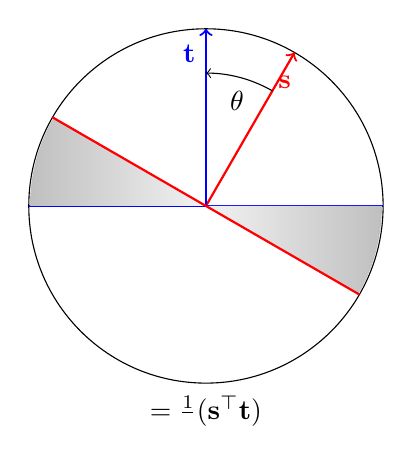
\begin{tikzpicture}[scale=1.5]

    % Circle
    \draw (0, 0) circle (1.5cm);

    % Vectors s (red at 60°) and t (blue at 90°)
    \draw[->,thick,red]  (0,0) -- (60:1.5cm) node[pos=0.7, above right] {\(\mathbf{s}\)};
    \draw[->,thick,blue] (0,0) -- (90:1.5cm) node[pos=0.75, above left] {\(\mathbf{t}\)};

    % Angle theta (between s & t)
    \draw[<-] (0,1.125) arc (90:60:1.125cm) node[pos=0.7, below left] {\(\theta\)};

    % Blue lines (perp. to t = 90°)
    \draw[thick,blue] (0,0) -- (-1.5,0);
    \draw[thick,blue] (0,0) -- ( 1.5,0);

    % Gray shading for overlap region
    \shade[left color=gray!50, right color=gray!10]
      (0,0) -- (-1.49,0) arc (180:150:1.5cm) -- cycle;
    \shade[left color=gray!10, right color=gray!50]
      (0,0) -- (1.49,0) arc (0:-30:1.5cm) -- cycle;

    % Red line(s) perp. to s (60°)
    \draw[thick,red]  (0,0) -- (150:1.5);
    \draw[thick,red]  (0,0) -- (330:1.5); % same as -30°

    % Overlap formula
    \node at (0,-1.75) {\( \AVGR = \frac{1}{\ND} (\mathbf{s}^\top \mathbf{t}) \)};

\end{tikzpicture}
\end{minipage}%
\hfill
%-------------------------------%
% Right image: 3D Overlap (conic sections + wedge)
%-------------------------------%
\begin{minipage}{0.48\linewidth}
\centering
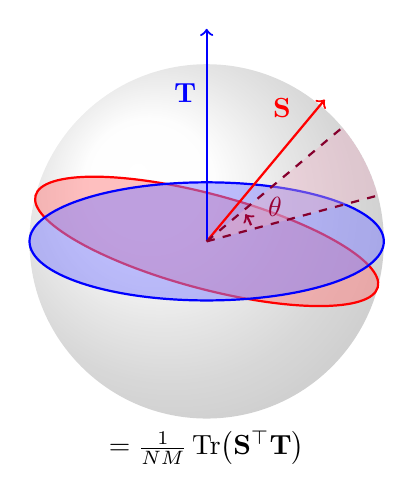
\begin{tikzpicture}[scale=1.5]

    % Light-gray "sphere"
    \shade[ball color=gray!5, opacity=0.3] (0,0) circle (1.5cm);

    % --- Red ellipse for S (unchanged) ---
    \begin{scope}
      \clip (0,0) circle (1.5cm);
      \fill[red!50, opacity=0.5]
        [rotate around={-15:(0,0)}, xscale=1.5, yscale=0.4]
        (0,0) circle (1.0);
    \end{scope}
    \draw[thick, red]
      [rotate around={-15:(0,0)}, xscale=1.5, yscale=0.4]
      (0,0) circle (1.0);

    % --- Blue ellipse for T (CHANGED) ---
    % Make it near-horizontal (rotate=0 or a small angle),
    % and bigger horizontally by increasing xscale significantly.
    \begin{scope}
      \clip (0,0) circle (1.5cm);
      \fill[blue!50, opacity=0.5]
        [rotate around={0:(0,0)},    % CHANGED: no tilt so near x-axis
         xscale=1.5, yscale=0.5]     % CHANGED: bigger horizontally
        (0,0) circle (1.0);
    \end{scope}
    \draw[thick, blue]
      [rotate around={0:(0,0)}, xscale=1.5, yscale=0.5]
      (0,0) circle (1.0);

    % Vectors S (red) & T (blue, vertical & longer)
    \draw[->,thick,red]  (0,0) -- (1.0,1.2)
      node[pos=0.8, above left]  {\(\mathbf{S}\)};
    \draw[->,thick,blue] (0,0) -- (0,1.8)
      node[pos=0.7, left] {\(\mathbf{T}\)};

    % Remove old "theta" arcs

    % -- Fill a wedge (solid angle) in purple --
    \begin{scope}
      \clip (0,0) circle (1.5cm);
      % Let’s pick a narrower wedge from ~15° to ~40°
      \fill[purple!30, opacity=0.4]
        (0,0)
         -- (15:1.5cm)
         arc [start angle=15, end angle=40, radius=1.5cm]
         -- cycle;
    \end{scope}

    % Dashed wedge boundaries
    \draw[thick, dashed, purple!70!black] (0,0) -- (15:1.5cm);
    \draw[thick, dashed, purple!70!black] (0,0) -- (40:1.5cm);

    % Single arc to label theta
    \draw[->, thick, purple!80!black]
      (20:0.4) arc[start angle=20, end angle=35, radius=0.4];
    \node[purple!80!black] at (27:0.65) {\(\theta\)};

    % Overlap formula
    \node at (0,-1.75) {\( \AVGR = \frac{1}{NM} \,\mathrm{Tr}\bigl(\mathbf{S}^\top \mathbf{T}\bigr) \)};

\end{tikzpicture}
\end{minipage}

% Main caption
\caption{Comparison of 2D and 3D representations of the vector and matrix Student--Teacher overlap \(R\).
\textbf{Left:} \(\AVGR = \tfrac{1}{\ND}\mathbf{s}^\top \mathbf{t}\).  Averaged over $\ND$ data samples (implicitly normalized to $1/m$).
\textbf{Right:} \(R = \tfrac{1}{NM}\,\mathrm{Tr}\bigl(\mathbf{S}^\top\mathbf{T}\bigr)\) with conic sections on the sphere (red \(\mathbf{S}\), blue \(\mathbf{T}\)), plus a purple wedge for the angle.  Averaged over matrix dimensions $N$ and $M$ (implicitly normalized over the data $1/\ND$).}
\label{fig:overlaps}
\end{figure}

%\caption{Comparison of 2D and 3D representations of matrix overlap $R$. (a) 2D visualization of vector overlap $R = \cos(\theta) $.
%  (b) 3D visualization of matrix overlap $R = \Trace{\frac{1}{N^2} \SMAT^\top \TMAT $ with solid angle $R$.}



%%\subsubsection{Derivation of the  ST error $(\EPSL(R))$ for the Linear Perceptron}
\paragraph{Derivation of the  ST error $(\EPSL(R))$ for the Linear Perceptron.}
%\nred{WARNING: there may be some mistakes here}
To derive \EQN~\ref{eqn:LinearPerceptronError},
define the data-dependent ST error (\EQN~\ref{eqn:DE_L}) in terms of an $\ell_2$ loss function
%\begin{align}
%\nonumber
%\Delta \mathbf{E}_{\ell_2}(\SVEC,\TVEC,\XI) = & \frac{1}{2} (\Ys - \Yt)^T(\Ys - \Yt) 
%   = 1 - (\YsVEC)^{\top}(\YtVEC) \\ 
%\label{eqn:deriveSTerror}
%   =&  1 - \eta(\XI),
%\end{align}

\begin{align}
\nonumber
\DETOPSTLL= & \frac{1}{2} (\YsVEC - \YtVEC)^{\top} (\YsVEC - \YtVEC) \\
\nonumber
=& \frac{1}{2} \big[(\YsVEC)^{\top} \YsVEC - 2 (\YsVEC)^{\top} \YtVEC + (\YtVEC)^{\top} \YtVEC \big] \\
\nonumber
=& N - (\YsVEC)^{\top} (\YtVEC) \\
\label{eqn:deriveSTerror}
=& N(1 - \ETA(\SVEC,\TVEC)),
\end{align}
where we call $\ETA(\SVEC,\TVEC,\XI):=\tfrac{1}{N}\mathbf{y}_{S}^{\top}\mathbf{y}_{T}$
the \emph{data-dependent \SelfOverlap}.
The expression $\ETA(\SVEC,\TVEC,\XI)$ is analogous to the ST overlap $R$, but before the data has been integrated out.
The \SelfOverlap $\ETA(\SVEC,\TVEC,\XI)$ will appear later in \EQN~\ref{eqn:eta2} (in Section~\ref{sxn:matgen}), 
when formulating the matrix-generalized overlap operator~$\OVERLAP$.

Using the $E_{NN}$ Energy generating or output function (\EQN~\ref{eqn:ENN}), we can replace the label vectors $\YtVEC,\YsVEC$ as
\begin{align}
\YsVEC=\SVEC^{\top}\XI,\;\;
\YtVEC=\TVEC^{\top}\XI  ,
\end{align}
which gives
\begin{align}
  \label{eqn:eta_vec_xi_def}
\ETA(\SVEC,\TVEC,\XI) = \tfrac{1}{N}(\SVEC^{\top}\XI)^{\top} (\TVEC^{\top}\XI) = \tfrac{1}{N}\XI^{\top} (\SVEC^{\top} \TVEC )\XI   .
\end{align}
or, more simply,
\begin{align}
  \label{eqn:eta_vec_avg_def}
\ETA(\SVEC,\TVEC) = \langle\ETA(\SVEC,\TVEC,\XI)\rangle_{\AVGNDXI}=\tfrac{1}{N}(\SVEC^{\top} \TVEC )
\end{align}

We want to evaluate this as an \EffectivePotential $\EPSL(R)$ for the data-averaged ST test error, as in \EQN~\ref{eqn:STerror}.
To do this, we need to compute the average or \ExpectedValue over all possible input data $\XI$,
an $N-$dimensional Gaussian vector (i.e., $d\mu(\XI)=\mathcal{D}\NDXI P(\NDXI)$).
%
%Using $\mathcal{N}$ as the normalization for the average, as yet unspecified, we obtain 
\nred{CHECK THIS: notice we do not include the $\tfrac{1}{N}$ on the R.H.S.}
\begin{align}
 \langle\DETOPSTLL\rangle_{\AVGNDXI}  
   = &\red{\cancel{\frac{1}{\mathcal{N}}}}\int d\mu(\NDXI)(1-\ETA(\XI)) \\ \nonumber
   = &\red{\cancel{\frac{1}{\mathcal{N}}}}\int d\mu(\NDXI)(1-\XI^{\top}\tfrac{1}{N}\SVEC^{\top}\TVEC\XI) \\ \label{eqn:XI_ST} 
   = &\red{\cancel{\frac{1}{\mathcal{N}}}\int d\mu(\NDXI)-\int d\mu(\NDXI)\XI^{\top}\tfrac{1}{N}\SVEC^{\top}\TVEC\XI) } \\ \nonumber
   = & \red{\cancel{\frac{N}{\mathcal{N}}}}1 - \int d\mu(\NDXI)\XI^{\top}\red{\tfrac{1}{N}}\SVEC^{\top}\TVEC\XI \\ \nonumber
   = & \red{\cancel{\frac{N}{\mathcal{N}}}}1 - \int d\mu(\NDXI)\red{\cancel{N}}\XI^{\top} R\XI \\ \nonumber
   = & \red{\cancel{\frac{N}{\mathcal{N}}}}1 - R\int d\mu(\NDXI)\XI^{\top}\XI,
\end{align}
where the fifth line holds because the elements of $\XI$ are i.i.d.\red{???}
Since $d\mu(\NDXI)$ is a measure over a (multi-variate) Gaussian distribution,
if we normalize the data vectors \red{ $\XI$ to $\frac{1}{\sqrt{M}}$ (See Section~\ref{app:st-gen-err-annealed-ham}),  then
\cancel{$\mathcal{N}=N$} the second term on the R.H.S. is unity?} and we recover (i.e., \red{\EQN~\ref{eqn:epsl}})
\begin{align}
\label{eqn:e0}
\EPSL(R)=\langle\DETOPSTLL\rangle_{\AVGNDXI} =  1 - R .
\end{align}
%%%
%%% CHM: what is this ?
%%\begin{align}
%%\frac{1}{N}\langle\Delta \mathbf{E}_{\ell_2}(\SVEC,\TVEC,\XI)\rangle_{\XI}  
%%= &\frac{1}{\mathcal{N}}\int d\mu(\XI)(1-\ETA(\XI)) \\ \nonumber
%%= &\frac{1}{\mathcal{N}}\int d\mu(\XI)(1-\XI^T\SVEC\TVEC^{\top}\XI) 
%%\end{align}
%%where $\mathcal{N}$ is the normalization for the average, as yet unspecified. Expanding, this gives
%%\begin{align}
%%\label{eqn:XI_ST}
%%\frac{1}{N}\langle\Delta \mathbf{E}_{\ell_2}(\SVEC,\TVEC,\XI)\rangle_{\XI} 
%%= & \frac{N}{\mathcal{N}} - \frac{1}{\mathcal{N}}\int d\mu(\XI)\XI^T\SVEC\TVEC^{\top}\XI \\ \nonumber
%%= & \frac{N}{\mathcal{N}} - \frac{1}{\mathcal{N}}\int d\mu(\XI)N\XI^T R\XI \\ \nonumber
%%= & \frac{N}{\mathcal{N}} - R\frac{N}{\mathcal{N}}\int d\mu(\XI)\XI^T\XI,
%%\end{align}
%%where the third line holds because the elements of $\XI$ are i.i.d.
%%Since $d\mu(\XI)$ is a measure over a Gaussian distribution, if we normalize the data vectors $\XI$ to $\frac{1}{\sqrt{N}}$, 
%%then $\mathcal{N}=N$, and we recover 
%%\begin{align}
%%\label{eqn:e0}
%%\EPSL(R)=\frac{1}{N}\langle\Delta \mathbf{E}_{\ell_2}(\SVEC,\TVEC,\XI)\rangle_{\AVGNDXI} =  1 - R .
%%\end{align}

\michaeladdressed{We have several types of subscripts on the BraKet average: $\NDXI$, $\XI$, and $\NDXIn$.  Im not sure if there are typos, or if things are overloaded. The difference isnt clear to me yet.}

In traditional \STATMECH (e.g., \cite{SST92}), one is interested in how the \emph{\TotalModelGeneralizationError} $\TGE(R)$ depends on $R$.
With these simple error functions, \EQN~\ref{eqn:MGE} reduces to a function over $R$,
and the \AverageSTGeneralizationError $\STGE(R)$ is then obtained by averaging over the Students 
\begin{align}
\label{eqn:AVGSTGE_R}
\AVGSTGE(R)=\THRMAVG{\EPSL(R)}=
\THRMAVG{1-\langle\ETA(\SVEC,\TVEC,\XI)\rangle_{\AVGNDXI}}=
\THRMAVG{1-\ETA(\SVEC,\TVEC)}=
\THRMAVG{1-\tfrac{1}{N}\SVEC^{\top}\TVEC}=
\THRMAVG{(1-R)}  ,
\end{align}
where $\THRMAVG{\cdots}$ is a \ThermalAverage over the \Student weight vector $\SVEC$.

Note that the \ModelQuality for the ST \Perceptron, $\Q^{ST}$
is just the \AverageGeneralizationAccuracy, so we can write
\begin{align}
\label{eqn:QST_final}
\Q^{ST} := 1 - \AVGSTGE(R) 
       = \THRMAVG{1 - \EPSL(R)} 
       = \THRMAVG{\langle\ETA(\SVEC, \TVEC, \XI)\rangle_{\AVGNDXI}} 
       = \THRMAVG{\ETA(\SVEC, \TVEC)} 
       = \THRMAVG{\tfrac{1}{N}\SVEC^{\top}\TVEC} 
       = \THRMAVG{R}.
\end{align}
\EQN~\ref{eqn:QST_final} is the starting point for deriving a \SEMIEMP theory for the \WW quality metrics (\ALPHA,\ALPHAHAT);
see Section~\ref{sxn:matgen_mlp3}.
To generalize this expression, we will start with the \SelfOverlap $\ETA(\SMAT,\TMAT,\XI)$ for a
\MultiLayerPerceptron (MLP3) in Section~\ref{sxn:matgen}.

Before doing this, however, we note that 
we can obtain this expression for $\STGE$ by defining the
\AnnealedHamiltonian $\HANHT(R)$, at high-Temperature, as in Section~\ref{sxn:mathP}, \EQN~\ref{eqn:Gan_highT_final}.
Indeed, it is really $\HANHT(R)=\EPSL(R)$ that we must generalize to the matrix case, which we do (using a technique
similar to a Replica calculation, but still in the AA).
For more details, see Appendix~\ref{sxn:summary_sst92}.
(In particular, doing this allows us to define the normalization needed later for the \TRACELOG condition).
\michaeladdressed{MM TO DO: still to work on this par.}


\begin{table}[t]
  \raggedright
\hspace*{-1.5cm}% Adjust this value as needed
\renewcommand{\arraystretch}{1.25} % Increase line spacing in table
\begin{tabular}{|c|c|c|c|}
  \hline
  Quantity & Traditional \SMOG & \makecell{\LinearPerceptron \\ in Traditional \SMOG} & \makecell{Matrix Generalization \\ for \SETOL} \\ \hline

  Total (Idealized) Data Error 
    & $\DETOPXI$ (\ref{eqn:detox})
    & $\DETOPSTL$ (\ref{eqn:deriveSTerror}) 
    & $\DETOPNN$ (\ref{eqn:DE2}) \\ \hline

   Annealed Hamiltonian
    & $\HANHT=\EPSLw$ (\ref{eqn:epsl}) 
    & $\GANHTR=\EPSLSTx=1-\AVGR$ (\ref{eqn:epslR}) 
  & $\GANMATHT = N(\IM-\OVERLAP)$ (\ref{eqn:GANHTmatR}) \\

  (Data-Averaged Error) 
    & (AA, at high-T) 
    & (and at \LargeN) 
    & (only for a layer)  \\ \hline

    \SelfOverlap 
    & $\ETAw = 1-\EPSLw$~(\ref{eqn:def_eta})

    & $\ETA(\SVEC,\TVEC)=\SVEC^{\top}\TVEC$ (\ref{eqn:eta_vec_avg_def})
    & $\ETA(\SMAT,\TMAT)=\tfrac{1}{N}\SMAT^{\top}\TMAT$ (\ref{eqn:eta_mat_avg_def})  \\ \hline
    \hline

  \ModelQuality 
    & $\Q:=1-\AVGGE$ 
    & $\Q^{ST}:=1-\AVGGE^{ST}$ (\ref{eqn:model_qualities})
   & $\Q^{NN}:=1-\AVGGE^{NN}$  (\ref{eqn:model_qualities})\\ 

  in terms of \LayerQuality
    & 
    & 
   & $\Q^{NN}:=\prod_{L} \Q^{NN}_{L}$ \\ \hline
\end{tabular}
\caption{Summary of key quantities compared across traditional \SMOG models,  the \Student-\Teacher (ST) \LinearPerceptron--in the \AnnealedApproximation
(AA) and at high-Temperature (high-T) and at \LargeN in $\ND$, and the matrix-generalized forms as the starting point to frame \SETOL.
The total ST Error of Energy, $\DELBF$, represents the difference (squared) between the model and its labels for the ST model between
the \Student and \Teacher predictions.
The \AnnealedHamiltonian is the Energy function for this Error after it is averaged over the model for the training data
(an $\ND$-dimensional i.i.d. idealized Gaussian dataset,  $\NDXIn$).
In the AA, the \AnnealedHamiltonian is equal to the \EffectivePotential.  For the ST model,  this is one minus the average overlap, $\HANHT(R)=(1-\AVGR)$;
for the \SETOL, this is  the ($M$-dimensional) identity minus the overlap operator/matrix, $\HANHT(\OVERLAP)=N(\IM-\OVERLAP)$. 
The \SelfOverlap $\eta(\cdots)$ is used to describe the Accuracy (as opposed to the Error) for both the ST model and
its matrix-generalized form.
%Notice that $\eta(\XI)$, as defined,  has not yet been averaged over the model data $\XI^{N}$.
Finally, the different forms of the \Quality are defined.  Generally speaking, the \Quality $\Q$ is an approximation to some measure
of $1$ minus the \AverageGeneralizationError, $\Q:=1-\AVGGE$ (in the AA, at high-T, at \LargeN, and with whatever else
approximations are applied).
For the ST model, having just 1 layer, the \ModelQuality and the \LayerQuality are the same, and denoted $\Q^{ST}$.
For \SETOL, the \ModelQuality $\Q^{NN}$ is a product of individual \LayerQualities $\Q^{NN}_{L}$.
(Note that the  final \SETOL \LayerQuality $\Q$ is defined in terms of the \LayerQualitySquared $\QT$,
and the starting point for this is expressed with the \LayerQualitySquared Hamiltonian $\HBARE=\OLAPTOLAP$.
}
\label{table:quantities_general_vect_matrix}
\end{table}


